%convert -coalesce launch.gif launch_%d.png
\documentclass{beamer}

\newcommand{\VEV}[1]{\langle#1\rangle}
\newcommand{\sst}{\left(1-\frac{2M}{r}\right)}
\newcommand{\sh}{\mathrm{shell}}
\newcommand{\be}{\begin{equation}}
\newcommand{\ee}{\end{equation}}
\newcommand{\bue}{\begin{equation}}
\newcommand{\eue}{\end{equation}}
\newcommand{\bc}{\begin{center}}
\newcommand{\ec}{\end{center}}
\newcommand{\bea}[1]{\begin{eqnarray}\label{#1}}
\newcommand{\eea}{\end{eqnarray}}
\newcommand{\bua}{\begin{eqnarray*}}
\newcommand{\eua}{\end{eqnarray*}}
\newcommand{\dd}[2]{{{d#1}\over{d#2}}}
\newcommand{\ddt}[1]{\dd{#1}{t}}
\newcommand{\dddt}[1]{\dd{^2#1}{t^2}}
\newcommand{\aver}[1]{\langle{#1}\rangle}
\newcommand{\atom}[3]{\ifmmode^{#1}_{#2}{\rm{#3}}\else{$^{#1}_{#2}${#3}}\fi}
\newcommand{\electron}{\atom{~0}{-1}{e}}
\newcommand{\positron}{\atom{0}{0}{\bar{e}}}
\newcommand{\neutrino}{\atom{0}{0}{\nu_e}}
\newcommand{\photon}{\atom{0}{0}{\gamma}}
\newcommand{\antineutrino}{\atom{0}{0}{\bar{\nu}}}
\newcommand{\neutron}{\atom{1}{0}{n}}
\newcommand{\proton}{\atom{1}{1}{p}}
\newcommand{\hydrogen}{\atom{1}{1}{H}}
\newcommand{\deuterium}{\atom{2}{1}{H}}
\newcommand{\tritium}{\atom{3}{1}{H}}
\newcommand{\helium}{\atom{4}{2}{He}}
\newcommand{\hethree}{\atom{3}{2}{He}}

\renewcommand{\ss}{Schwarz\-schild }

\def\densu{kg/m$^3$} 
\def\rsol{R$_{\odot}$} 
\def\msol{M$_{\odot}$} 


\usetheme{Boadilla}
%\usepackage{multimedia}
%\usepackage{animate}
\usepackage{hyperref}
\usepackage{tikz}
\usepackage{cancel}
\usepackage{tikzsymbols}
\usepackage{ifthen}

%%%%mathcircled
\makeatletter
\newcommand\mathcircled[1]{%`
  \mathpalette\@mathcircled{#1}%
}
\newcommand\@mathcircled[2]{%
  \tikz[baseline=(math.base)] \node[draw,circle,red, thick, inner sep=2pt] (math) {$\m@th#1#2$};%
}
\makeatother
%%%%

%gets rid of bottom navigation bars
\setbeamertemplate{footline}[frame number]{} %begin

%gets rid of bottom navigation symbols
\setbeamertemplate{navigation symbols}{}

%gets rid of footer
%will override 'frame number' instruction above  %begin
%comment out to revert to previous/default definitions
\setbeamertemplate{footline}{}

\definecolor{darkscarlet}{rgb}{0.34, 0.01, 0.1}
\definecolor{gold(metallic)}{rgb}{0.83, 0.69, 0.22}
\definecolor{green(ryb)}{rgb}{0.4, 0.69, 0.2}
\definecolor{darkorange}{rgb}{1.0, 0.55, 0.0}
\definecolor{amber}{rgb}{1.0, 0.75, 0.0}
\definecolor{bronze}{rgb}{0.8, 0.5, 0.2}
\definecolor{cadet}{rgb}{0.33, 0.41, 0.47}
\definecolor{silver}{rgb}{0.75, 0.75, 0.75}
\definecolor{turquoise}{rgb}{0.19, 0.84, 0.78}
\definecolor{uclagold}{rgb}{1.0, 0.7, 0.0}
\definecolor{urobilin}{rgb}{0.88, 0.68, 0.13}
\definecolor{vegasgold}{rgb}{0.77, 0.7, 0.35}
\definecolor{vanilla}{rgb}{0.95, 0.9, 0.67}
\definecolor{straw}{rgb}{0.89, 0.85, 0.44}
\definecolor{sunset}{rgb}{0.98, 0.84, 0.65}
\definecolor{brown(traditional)}{rgb}{0.59, 0.29, 0.0}
\definecolor{apricot}{rgb}{0.98, 0.81, 0.69}
\definecolor{darkblue}{rgb}{0,0,0.54}
\definecolor{denim}{rgb}{0.06, 0.29, 0.55}

\hypersetup{
    colorlinks=true,
    linkcolor=yellow,
    filecolor=magenta,
    urlcolor=blue,
}

\let\hrefori\href
\renewcommand{\href}[2]{{\setlength{\fboxsep}{1pt}\colorbox{sunset}{\hrefori{#1}{#2}}}}

%Schwarzschild command
\renewcommand{\ss}{Schwarz\-schild }

%title
\setbeamercolor{block title alerted}{fg=white,bg=cyan}
%body
\setbeamercolor{block body alerted}{fg=black!90,bg=yellow!60}

%title
\setbeamercolor{block title}{fg=black,bg=turquoise}
%body
\setbeamercolor{block body}{fg=yellow,bg=bronze}




\newcommand{\pagebutton}[1]{\setbeamertemplate{button}{\tikz\node[inner xsep = 5pt, draw = structure!90, fill = green(ryb), rounded corners = 8pt]{\color{amber}\Large\insertbuttontext};}\beamerbutton{#1}}

\newcommand{\choicebutton}[1]{\setbeamertemplate{button}{\tikz\node[inner xsep = 8pt, draw = structure!90, fill = vegasgold, rounded corners = 5pt]{\color{vanilla}\Large\insertbuttontext};}\beamerbutton{#1}}

\newcommand{\pagenobutton}[1]{\setbeamertemplate{button}{\tikz\node[inner xsep = 8pt, draw = structure!90, fill = apricot, rounded corners = 5pt]{\color{brown(traditional)}\Large\insertbuttontext};}\beamerbutton{#1}}

\newcommand{\headlinebutton}[1]{\setbeamertemplate{button}{\tikz\node[inner xsep = 8pt, draw = structure!90, fill = blue, rounded corners = 5pt]{\color{yellow}\Large\insertbuttontext};}\beamerbutton{#1}}

\newcommand{\forumbutton}{\href{https://astro-discourse.utenforuio.no/c/ast2000/sporsmal-til-ukeoppgavene-i-del-2a-2d/11}{\setbeamertemplate{button}{\tikz\node[inner xsep = 8pt, draw = structure!90, fill = darkblue, rounded corners = 5pt]{\color{yellow}\Large\insertbuttontext};}\beamerbutton{\textcolor{red}{\small FORUM}}}}

\newcommand{\curpage}{\pagenobutton{\small side \thepageno\  av \thenopages}}
\newcommand{\nextpage}{\refstepcounter{pageno}\pagenobutton{\small side \thepageno\  av \thenopages}}
\newcommand{\dnextpage}{\refstepcounter{pageno}\refstepcounter{pageno}\pagenobutton{\small side \thepageno\  av \thenopages}}

\newcommand{\lastpagebutton}[1]{\hyperlink{#1}{\pagebutton{\small Forrige side}}\href{https://nettskjema.no/a/171674}{\Changey[1][yellow]{2} \Changey[1][yellow]{-2}}\nextpage\headlinebutton{\headline}\forumbutton}
\newcommand{\clastpagebutton}[1]{\hyperlink{#1}{\pagebutton{\small Forrige side}}\href{https://nettskjema.no/a/171674}{\Changey[1][yellow]{2} \Changey[1][yellow]{-2}}\curpage\headlinebutton{\headline}\forumbutton}
\newcommand{\dlastpagebutton}[1]{\hyperlink{#1}{\pagebutton{\small Forrige side}}\href{https://nettskjema.no/a/171674}{\Changey[1][yellow]{2} \Changey[1][yellow]{-2}}\dnextpage\headlinebutton{\headline}\forumbutton}

\newcommand{\lastpagebuttonx}[1]{\hyperlink{#1}{\pagebutton{\small Forrige side}}\href{https://nettskjema.no/a/171674}{\Changey[1][yellow]{2} \Changey[1][yellow]{-2}}\nextpage\\}
\newcommand{\clastpagebuttonx}[1]{\hyperlink{#1}{\pagebutton{\small Forrige side}}\href{https://nettskjema.no/a/171674}{\Changey[1][yellow]{2} \Changey[1][yellow]{-2}}\curpage\\}
\newcommand{\dlastpagebuttonx}[1]{\hyperlink{#1}{\pagebutton{\small Forrige side}}\href{https://nettskjema.no/a/171674}{\Changey[1][yellow]{2} \Changey[1][yellow]{-2}}\dnextpage\\}

\newcommand{\lastpagebuttoncr}[1]{\hyperlink{#1}{\pagebutton{\small Forrige side}}\href{https://nettskjema.no/a/171674}{\Changey[1][yellow]{2} \Changey[1][yellow]{-2}}\nextpage\\\headlinebutton{\headline}\forumbutton\\}
\newcommand{\clastpagebuttoncr}[1]{\hyperlink{#1}{\pagebutton{\small Forrige side}}\href{https://nettskjema.no/a/171674}{\Changey[1][yellow]{2} \Changey[1][yellow]{-2}}\curpage\\\headlinebutton{\headline}\forumbutton\\}
\newcommand{\dlastpagebuttoncr}[1]{\hyperlink{#1}{\pagebutton{\small Forrige side}}\href{https://nettskjema.no/a/171674}{\Changey[1][yellow]{2} \Changey[1][yellow]{-2}}\dnextpage\\\headlinebutton{\headline}\forumbutton\\}

\newcommand{\nytemaside}[1]{
\centerline{\Huge\textcolor{yellow}{Nytt tema:}}\\
\vspace*{1cm}
\centerline{\Large\bf\textcolor{yellow}{\headline}}
\vspace*{2cm}
\ifthenelse{\equal{#1}{0}}{\centerline{\textcolor{yellow}{Siste tema i denne forelesningen!}}}{\centerline{\textcolor{yellow}{\footnotesize Dette temaet fortsetter frem til side \ref{#1} av \thenopages.}}}
\vspace*{0.5cm}
}


\newcommand{\fullframe}[6]{
\begin{frame}
\label{#1}
\addtocounter{pageno}{#4}
\lastpagebutton{#2}{\bf #6}\\
#5
\hyperlink{#3}{\pagebutton{Neste side}}
\end{frame}
}



\newcommand{\fullframetwo}[7]{
\begin{frame}
\label{#1}
\addtocounter{pageno}{#4}
\lastpagebutton{#2}{\bf #7}\\
\begin{columns}
\column{0.5\textwidth}
#5
\column{0.5\textwidth}
#6
\hyperlink{#3}{\pagebutton{Neste side}}
\end{columns}
\end{frame}
}

\newcommand{\fullframetwonotxt}[7]{
\begin{frame}
\label{#1}
\addtocounter{pageno}{#4}
\lastpagebutton{#2}{\bf #7}\\
\begin{columns}
\column{0.5\textwidth}
#5
\column{0.5\textwidth}
#6
\end{columns}
\end{frame}
}



\newcommand{\fullframetxt}[7]{
\begin{frame}
\label{#1}
\addtocounter{pageno}{#4}
\lastpagebutton{#2}{\bf #7}\\
#6
\hyperlink{#3}{\pagebutton{#5}}
\end{frame}
}

\newcommand{\fullframenotxt}[6]{
\begin{frame}
\label{#1}
\addtocounter{pageno}{#4}
\lastpagebutton{#2}{\bf #6}\\
#5
\end{frame}
}

\newcommand{\choiceframe}[5]{
\begin{frame}
\label{#1}
\addtocounter{pageno}{#3}
\lastpagebutton{#2}{\bf #5}\\
#4
\end{frame}
}

\newcommand{\colfullframe}[7]{
{
\setbeamercolor{background canvas}{bg=#5}
\begin{frame}
\label{#1}
\addtocounter{pageno}{#4}
\lastpagebutton{#2}{\bf #7}\\
#6
\hyperlink{#3}{\pagebutton{Neste side}}
\end{frame}
}
}

\newcommand{\colfullframenotxt}[7]{
{
\setbeamercolor{background canvas}{bg=#5}
\begin{frame}
\label{#1}
\addtocounter{pageno}{#4}
\lastpagebutton{#2}{\bf #7}\\
#6
\end{frame}
}
}

\newcommand{\colfullframetwo}[8]{
{
\setbeamercolor{background canvas}{bg=#5}
\begin{frame}
\label{#1}
\addtocounter{pageno}{#4}
\lastpagebutton{#2}{\bf #8}\\
\begin{columns}
\column{0.5\textwidth}
#6
\column{0.5\textwidth}
#7
\hyperlink{#3}{\pagebutton{Neste side}}
\end{columns}
\end{frame}
}
}

\newcommand{\colfullframetxt}[8]{
{
\setbeamercolor{background canvas}{bg=#5}
\begin{frame}
\label{#1}
\addtocounter{pageno}{#4}
\lastpagebutton{#2}{\bf #8}\\
#7
\hyperlink{#3}{\pagebutton{#6}}
\end{frame}
}
}

\newcommand{\colchoiceframe}[6]{
{
\setbeamercolor{background canvas}{bg=#4}
\begin{frame}
\label{#1}
\addtocounter{pageno}{#3}
\lastpagebutton{#2}{\bf #6}\\
#5
\end{frame}
}
}


\newcommand{\pagequestion}[3]{
\hyperlink{#1}{\pagebutton{#2}}
\pause
%#3 normalt -1 for første spørsmål
\addtocounter{pageno}{#3}
\begin{itemize}[<+->]
\item[] \hypertarget<.>{#1}{}
\end{itemize}
\vspace{-0.5cm}
}

\newcommand{\samepagequestion}[4]{
\hyperlink{#1}{\pagebutton{#2}}\hyperlink{#1}{\pagebutton{#3}}
\pause
%#3 normalt -1 for første spørsmål
\addtocounter{pageno}{#4}
\begin{itemize}[<+->]
\item[] \hypertarget<.>{#1}{}
\end{itemize}
\vspace{-0.5cm}
}

\newcommand{\twopagequestion}[7]{
\hyperlink{#1}{\pagebutton{#3}}\hyperlink{#2}{\pagebutton{#4}}
\pause
%#3 normalt -1 for første spørsmål
\addtocounter{pageno}{#5}
\begin{itemize}[<+->]
\item[] \hypertarget<.>{#1}{}
\end{itemize}
\vspace{-0.5cm}
#7
\addtocounter{pageno}{#6}
\begin{itemize}[<+->]
\item[] \hypertarget<.>{#1}{}
\end{itemize}
\vspace{-0.5cm}
}

\newcounter{pageno}
\newcounter{nopages}
\setcounter{nopages}{42}

\newcommand{\headline}{\small Introduksjon}
\newcommand{\m}{\mathrm{m}}

\begin{document}

\begin{frame}
\label{front2}
\center{\Large \textcolor{darkscarlet}{\bf AST2000 Del 2C\\Interaktive forelesningsnotater: forelesning 2 av 2}}\\
\begin{block}{\center{\bf VIKTIG}}
\textcolor{yellow}{Dette er et alternativ til forelesningen i emnet.} \textcolor{blue}{Har du gått skikkelig gjennom disse interaktive forelesningsnotatene så trenger du ikke å lese \href{https://www.uio.no/studier/emner/matnat/astro/AST2000/h21/undervisningsmateriell/lecture_notes/part2c.pdf}{de fulle forelesningsnotatene} (med unntak av oppgavene bak)}. All informasjonen du trenger, får du her. Du kommer til å få mange grublespørsmål og diskusjonsoppgaver, det er meningen at disse skal gjøres i grupper av minst 2, maks 4 studenter. {\bf Det er defor sterkt anbefalt at dere sitter sammen i grupper når dere går gjennom disse interaktive forelesningsnotatene, du vil få betydelig mer utbytte av dem på den måten}. {\bf Hvis du har kommentarer ris/ros til disse forelesningsnotatene eller til emnet, trykk på \href{https://nettskjema.no/a/171674}{\Changey[1][yellow]{2} \Changey[1][yellow]{-2}}\ knappen som du finner på alle sider.}
\end{block}
%\setbeamercolor{button}{bg=black,fg=yellow}
\hyperlink{front3}{\pagebutton{Trykk denne knappen for å begynne}}
\end{frame}

\begin{frame}
\label{front3}
{\Large
\begin{itemize}
\item HUSK at du får mer ut av de interaktive forelesningsnotatene når du gjør de sammen med noen. Diskusjonene med andre er svært viktige.
\item Det er mange spørsmål/grubliser underveis, sett dere selv en tidsgrense, 1 minutt på de korte, maks 4-5 minutter på de lenger. Ha en alarm ved siden av, ellers kommer dere til å bruke alt for langt tid. Har dere ikke fått det til etter kort tid, gå videre, se svaret og lær!
\item Er du i det minste tvil om noe, så finnes det en \forumbutton knapp, trykk det og still spørsmål med en gang mens du enda husker spørsmålet!
\end{itemize}
}
\hyperlink{tableofcontents}{\pagebutton{Trykk denne knappen for å begynne}}
\end{frame}

\begin{frame}
\label{tableofcontents}
\hyperlink{front3}{\pagebutton{Forrige side}}\\
Hvis du allerede har begynt på denne forelesningen og vil hoppe rett inn til et annet kapittel, kan du trykke her:
\begin{itemize}
\item \hyperlink{blue_nytema1}{\headlinebutton{Maksimal aldring i Lorentzgeometri}}
\item \hyperlink{denim_ma21}{\headlinebutton{Maksimal aldring i Schwarzschildgeometri}}
\item \hyperlink{blue_nytema2}{\headlinebutton{Falling, falling...}}
\item \hyperlink{blue_nytema3}{\headlinebutton{GPS}}
\end{itemize}
Merk at sidene er merket med sidenummer på denne måten: SIDE X/Y/Z. Her er Z antall sider totalt, Y er sidenummeret til siste side i avsnittet du holder på med og X er sidenummeret til siden du er på.\\
\hyperlink{feil_intro}{\choicebutton{Neste side}}
\end{frame}

%%%%% intro
{
\setbeamercolor{background canvas}{bg=black}
\begin{frame}
\label{feil_intro}
\begin{columns}
\column{0.5\textwidth}
\hyperlink{front3}{\pagebutton{Forrige side}}\\
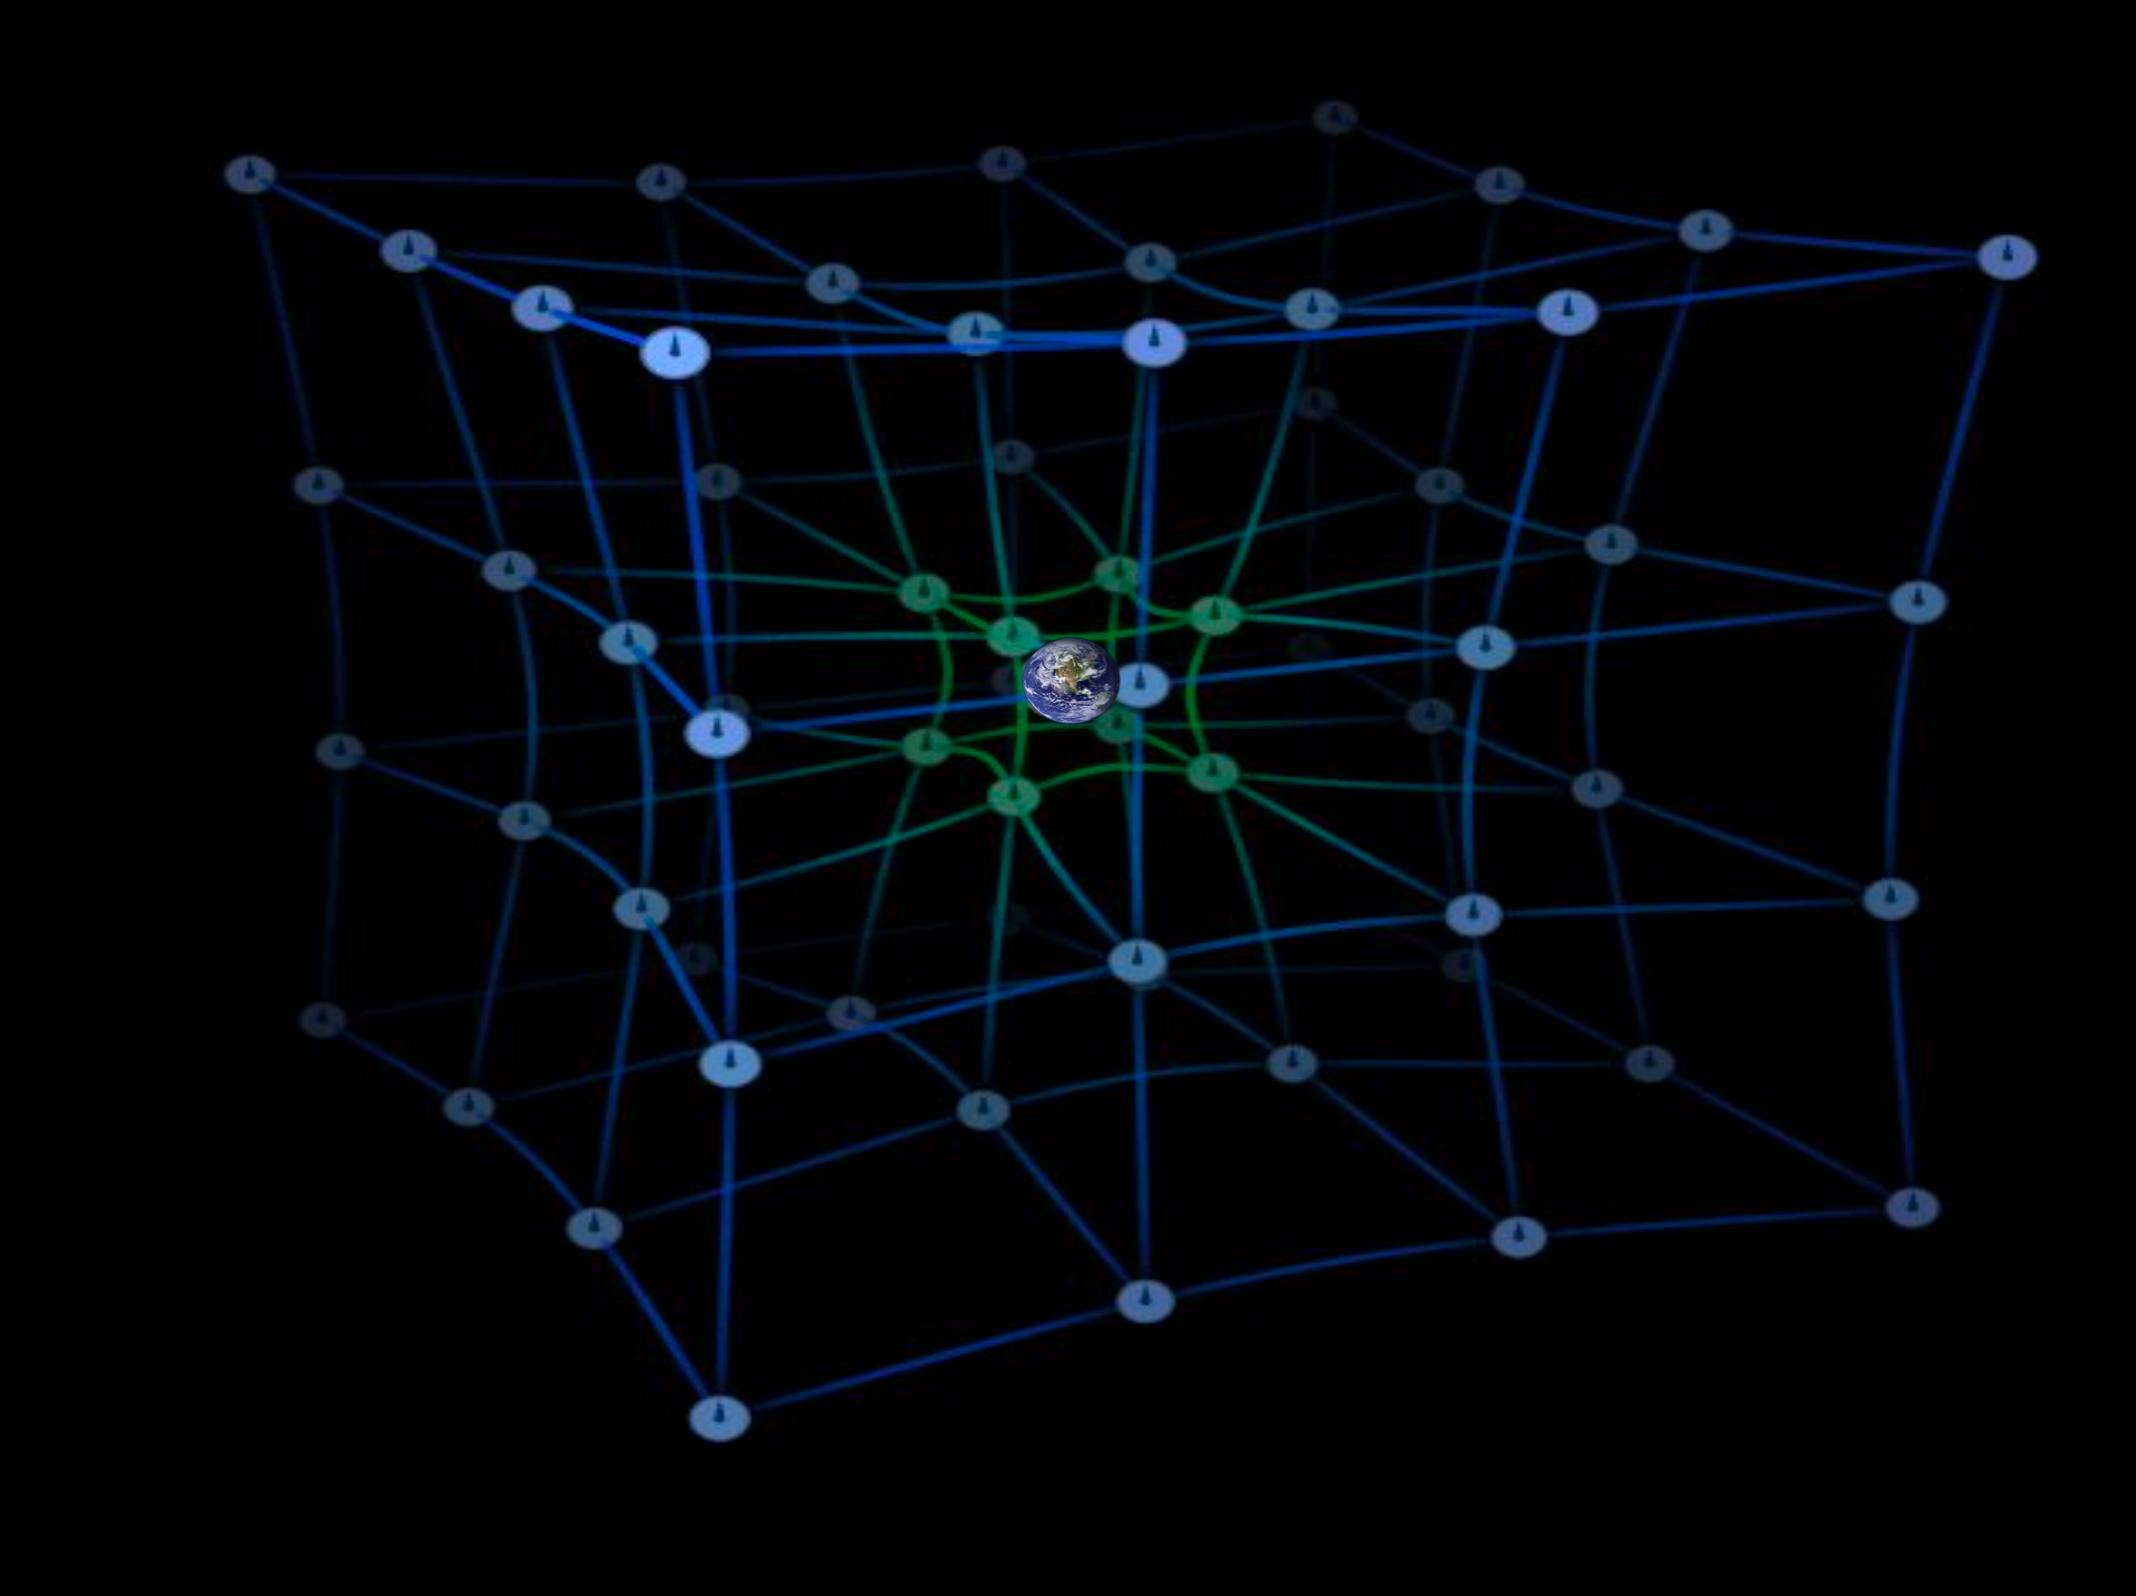
\includegraphics[scale=0.25]{media/spacetimebending.png}
\column{0.5\textwidth}
{\small
\textcolor{yellow}{\bf Velkommen til forelesning 2 av 2 i del 2C! Vi skal nå regne med \ss-geometri. Først skal vi tilbake til prinsippet for maksimal aldring og se hvilke store konsekvenser dette prinsippet har i et krumt tidrom. Så skal vi se på en stakkar som faller inn i et sort hull og så skal vi se på praktisk anvendelse av generell relativitetsteori: visst du at den er helt nødvendig for å få GPS til å funke? Normalt tar dette forelesningsnotatet en og en halv dobbelttime (altså 3 klokketimer).}\\
\textcolor{red}{Fremstillingen av generell relativitetsteori i AST2000 er basert på den fantastiske boken ``Exploring black holes'' av E. Taylor, J. Wheeler og E. Bertschinger, gratis tilgjengelig \href{http://www.eftaylor.com/exploringblackholes/}{her}. Anbefales på det sterkeste for den som er interessert.}
{(\tiny Illustrasjon fra pngegg.com)}}
\hyperlink{intro2}{\pagebutton{Neste side}}
\end{columns}
\end{frame}
}


\begin{frame}`
\label{intro2}
\lastpagebutton{feil_intro}
\begin{alertblock}{Vi begynner som vanlig...}
...med litt brainstorming. Som det er {\bf svært viktig} at du gjør før du går videre.
\end{alertblock}
\href{https://nettskjema.no/a/172649}{\begin{minipage}{5cm}Trykk her for å varme opp\end{minipage}}\\
Er du klar og har sendt inn skjemaet?
\href{https://nettskjema.no/a/172649}{\choicebutton{Nei}}\ \ \ \ \hyperlink{blue_nytema1}{\choicebutton{Ja}}\\
\end{frame}

\renewcommand{\headline}{Maksimal aldring}
{
\setbeamercolor{background canvas}{bg=blue}
\begin{frame}
\label{blue_nytema1}
\hyperlink{intro2}{\pagebutton{\small Forrige side}}
\nytemaside{ff}
\textcolor{yellow}{\Large Normalt kommer jeg omtrent frem til avsnittet om GPS i den fysiske forelesningen og tar resten forelesningen etter. Det anbefaler jeg at du også gjør! Vi skal nå snakke om maksimal aldring og ta en liten pause midtveis før neste tema.}
\hyperlink{ma1}{\pagebutton{Maksimal aldring revisited...}}
\end{frame}
}


\fullframe{ma1}{intro2}{ma2}{1}{\Huge
Vi begynner med den siste sida fra forrige forelesning: Hvis du ikke husker helt hva vi drev med anbefales det sterkt å ta en titt på oppsummeringen i \href{https://www.uio.no/studier/emner/matnat/astro/AST2000/h20/undervisningsmateriell/interaktive-forelesningsnotater/2c/videoer/video2c_4.mp4}{denne videoen} slik at du er klar for det som nå kommer...
}{SIDE 1/31/63}

\fullframe{ma2}{ma1}{ma3}{0}{\huge
Husker du prinsippet om maksimal aldring? I \href{https://www.uio.no/studier/emner/matnat/astro/AST2000/h20/undervisningsmateriell/interaktive-forelesningsnotater/2b/videoer/video2b_9.mp4}{denne videoen} fra del 2B får du en oversikt over prinsippet og hvordan det kan brukes til å vise Newtons 1.lov i et inertialsystem med Lorentzgeometri. Hvis du ikke husker helt hvordan det var, kikk gjennom videoen nå før du går videre!
}{SIDE 2/31/63}


\fullframe{ma3}{ma2}{ma4}{0}{\Large
Vi skal nå vise det som ble hoppet glatt over i videoen, nemlig hvorfor den rette linja er den {\bf lengste} veien i tidrommet når vi har Lorentzgeometri. Vi tar derfor en kjapp tur tilbake til spesiell relativitetsteori siden vi etterpå skal bruke den samme metoden på generell relativitetsteori og \ss-geometri.
}{SIDE 3/31/63}


\fullframe{ma4}{ma3}{ma5x}{0}{
\centerline{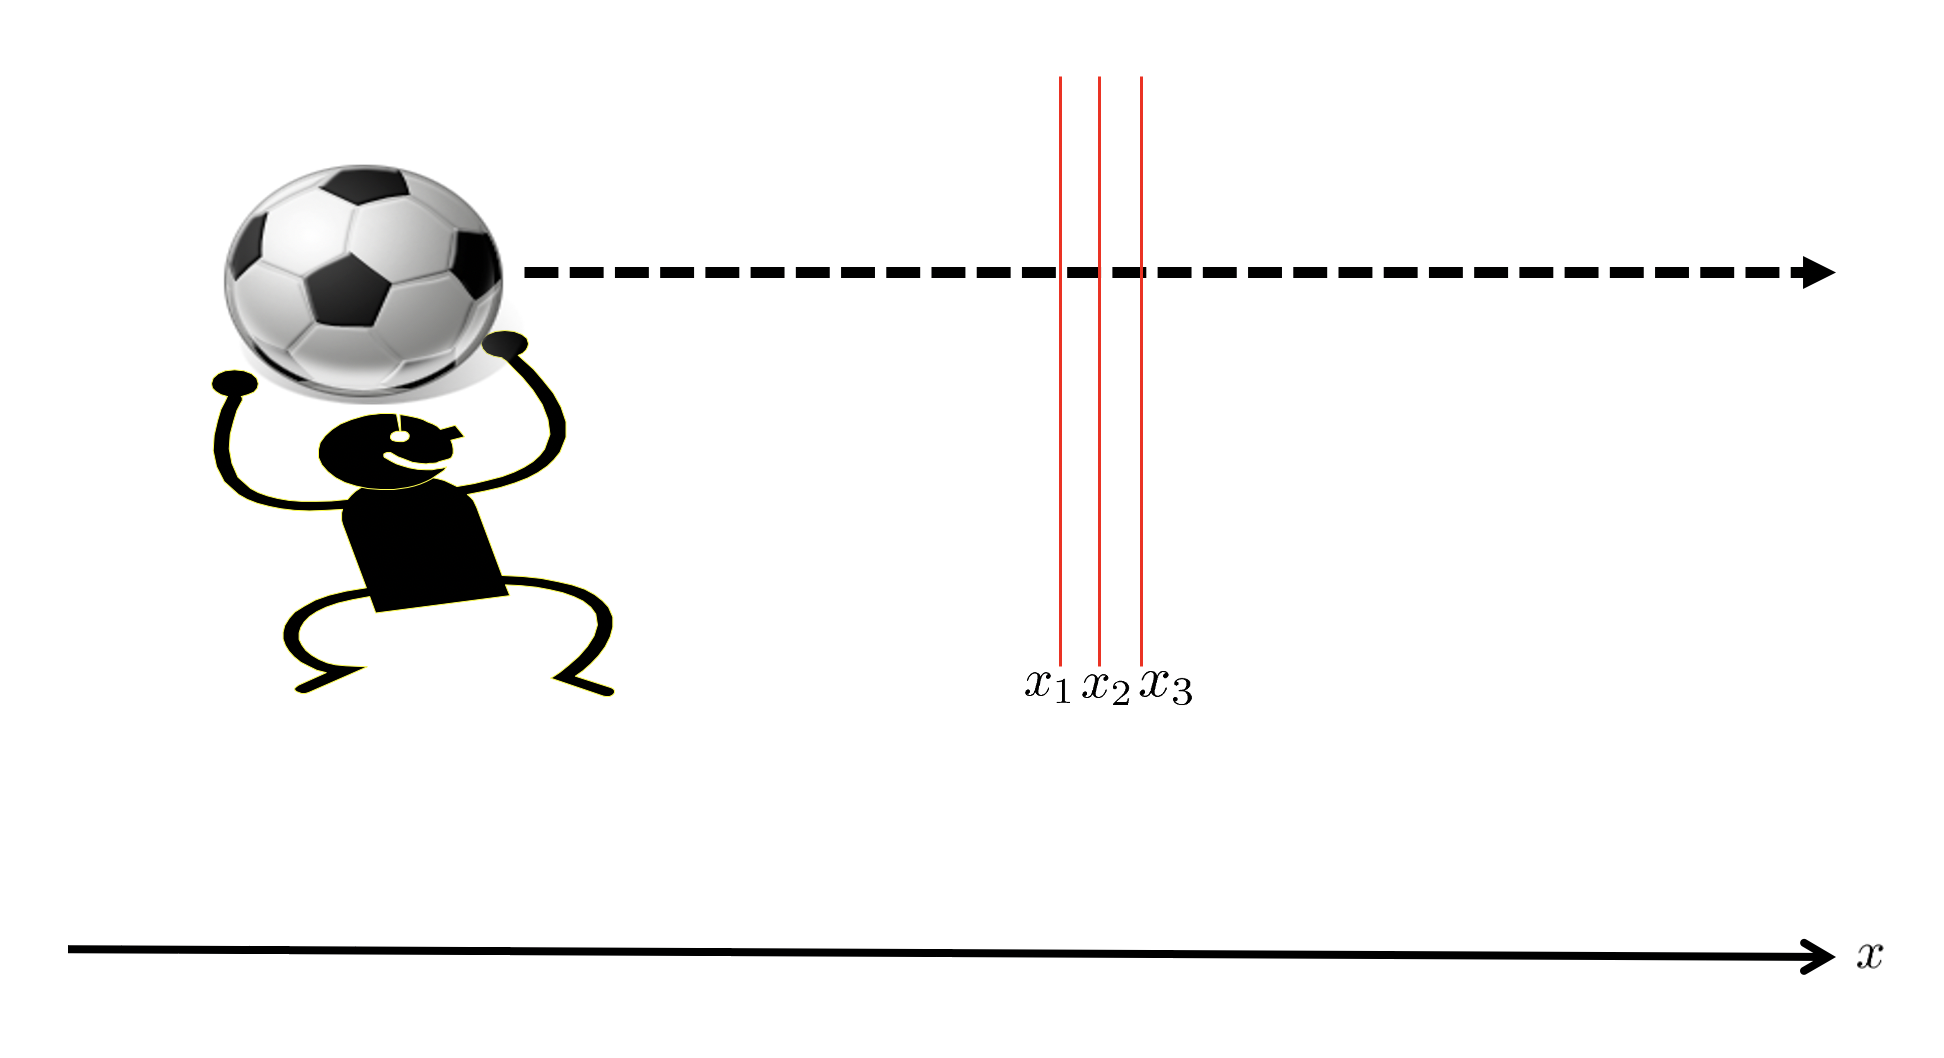
\includegraphics[scale=0.22]{media/maks_aldring2.png}}
Her ser vi en person som kaster en ball rett bortover x-aksen. Personen befinner seg i et inertialsystem. Det virker altså ingen krefter eller gravitasjon i dette systemet. Vi har så tatt ut en infinitesimal liten del av veien som ballen følger. Vi gjør denne delen av veien er så liten at vi fra posisjon $x_1$ til $x_2$ kan anta at hastigheten er konstant lik $v_A$. Og helt tilsvarende for avstanden fra $x_2$ til $x_3$ der hastigheten er konstant lik $v_B$ i hele intervallet. Merk at $v_A$ og $v_B$ ikke nødvendigvis er like, vi må være åpne for muligheten for at ballen kan akselerere underveis.
}{SIDE 4/31/63}

\fullframe{ma5x}{ma4}{ma5}{0}{
\centerline{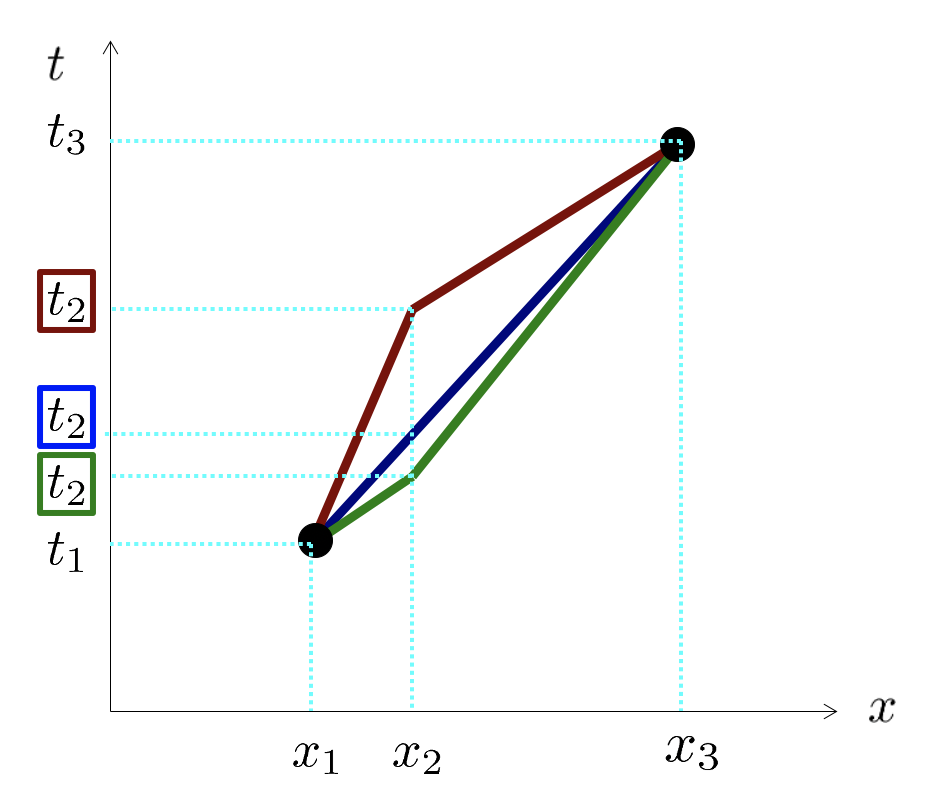
\includegraphics[scale=0.22]{media/maks_aldring1.png}}
Her ser vi tidromdiagram av situasjonen med tilhørende mulige verdenslinjer. Igjen så ser vi altså bare på en infinitesimal liten del av verdenslinja, to linjestykker som er infinitesimalt små der ballen har konstant hastighet (altså rett linje i tidrommet). Vi ser 3 {\bf mulige} verdenslinjer integnet her av {\bf uendelig mange mulige verdenslinjer} fra $x_1$ til $x_3$. \textcolor{red}{Vi vet ikke hvilken av de uendelig mange verdenslinjene ballen faktisk tar, det er det vi nå skal bruke prinsippet om maksimal aldring til å finne ut.}{\footnotesize (Dvs. vi vet det jo egentlig, men vi later som om vi ikke vet det for å kunne utlede det!)}
}{SIDE 5/31/63}


\choiceframe{ma5}{ma5x}{0}{
\centerline{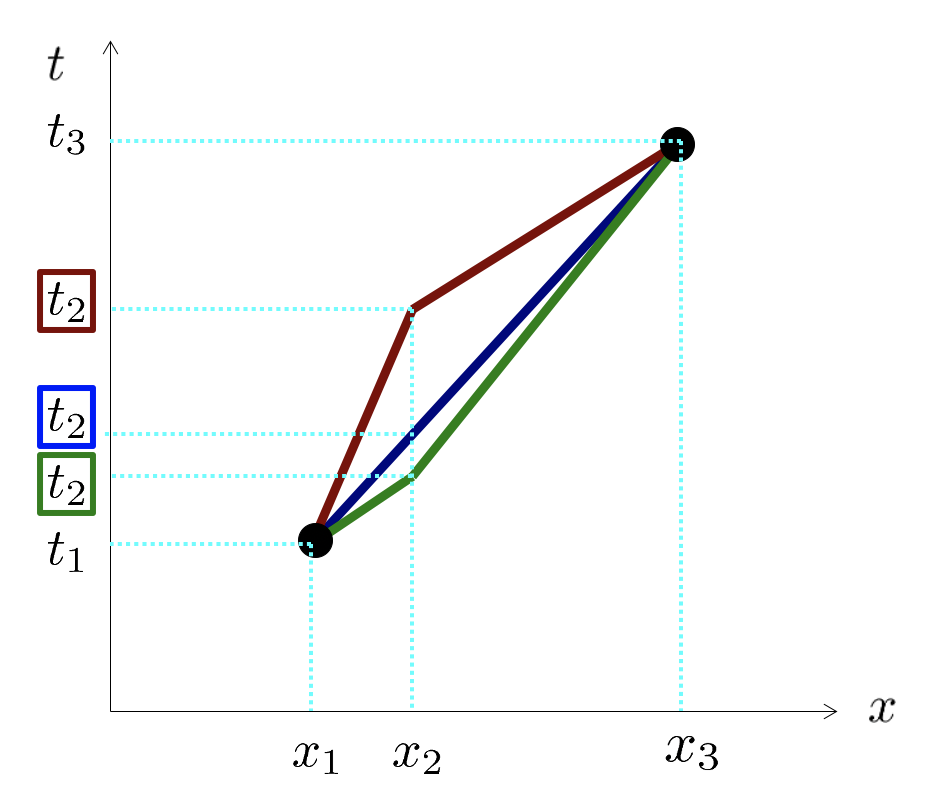
\includegraphics[scale=0.3]{media/maks_aldring1.png}}
Bare et av disse utsagnene er riktig, trykk på det riktige:
\hyperlink{feil_ma5a}{\choicebutton{rød sakker farten, grønn øker farten}}\\
\hyperlink{feil_ma5a}{\choicebutton{grønn sakker farten, blå øker farten}}\\
\hyperlink{riktig_ma5b}{\choicebutton{grønn sakker farten, rød øker farten}}\\
\hyperlink{feil_ma5a}{\choicebutton{blå sakker farten, rød øker farten}}
}{SIDE 6/31/63}

\colchoiceframe{feil_ma5a}{ma5}{0}{black}{
\centerline{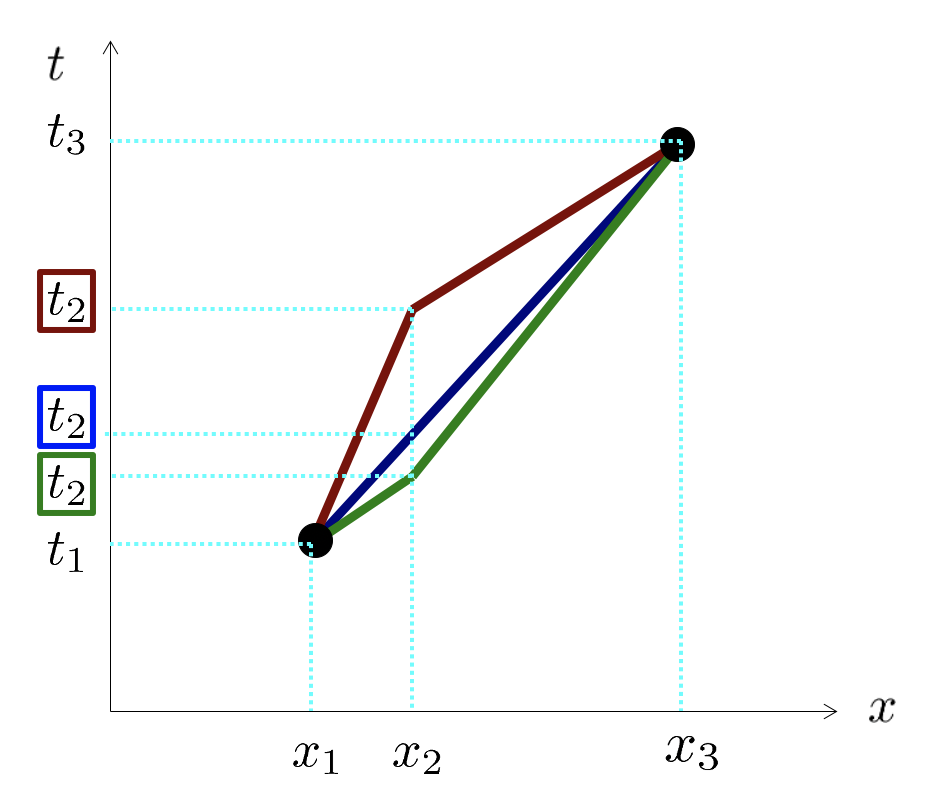
\includegraphics[scale=0.3]{media/maks_aldring1.png}}
\textcolor{yellow}{
Det ble vel ikke helt riktig? Husker du hvordan sammenhengen mellom fart og helning på linja er? Hvis ikke, ta en kikk nå på forelesningsnotatene for \href{https://www.uio.no/studier/emner/matnat/astro/AST2000/h20/undervisningsmateriell/lecture_notes/part2c.pdf}{del 2B}! Husk at fart er endring i posisjon $\Delta x$ delt på tidsintervall $\Delta t$. Prøv igjen!
}
}{SIDE 7/31/63}

\colfullframe{riktig_ma5b}{ma5}{ma6}{-1}{yellow}{\Large
\centerline{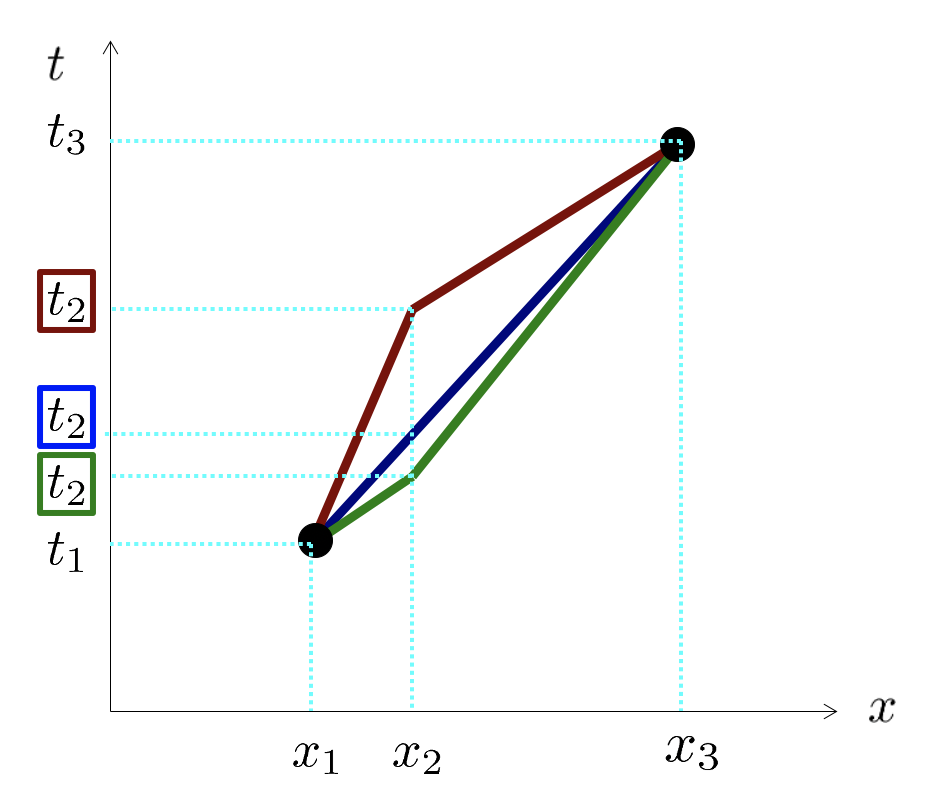
\includegraphics[scale=0.22]{media/maks_aldring1.png}}
Det er helt riktig. Du har kontroll på verdenslinjene og kan fortsette!
}{SIDE 8/31/63}


\fullframetxt{ma6}{ma5}{ma7}{0}{\small Neste side}{\small
\centerline{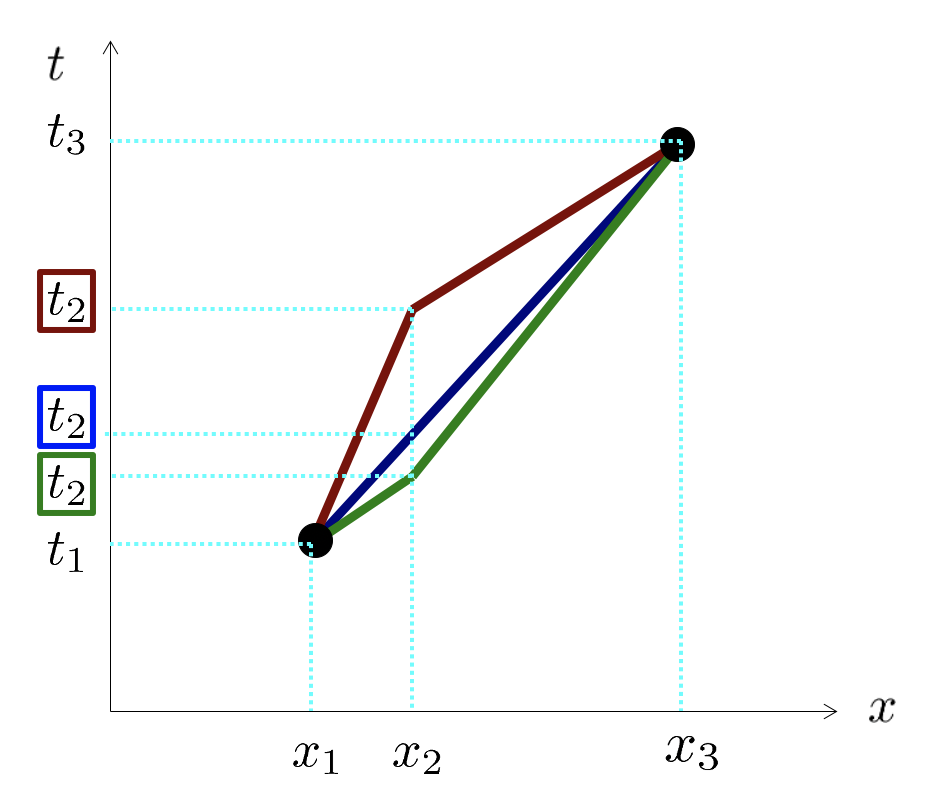
\includegraphics[scale=0.3]{media/maks_aldring1.png}}
Det vi ikke vet her er endringen i hastighet fra $v_A$ til $v_B$. Vi antar nå at alle posisjonene $x_1$, $x_2$ og $x_3$ er kjent. Vi antar også at tidspunktene $t_1$ og $t_3$ er kjent. Det som er ukjent er tidspunktet som ballen er i posisjon $x_2$. Hvis vi kan bruke prinsippet om maksimal aldring til å fortelle oss tidspunktet $t_2$, ja da vet vi hele verdenslinja fra $x_1$ til $x_3$. Det gjør at vi også vil vite om objektet tok en rett linje i tidrommet eller om det endret fart underveis. I figuren ser du de mulige tidspunktene $t_2$ for de 3 linjene som er opptegnet. Vi ser at hvis prinsippet om maksimal aldring gir oss tidspunktet $t_2$ som tilsvarer den blå linja, så har vi vist at ballen tar en rett linje med konstant fart i tidrommet.
}{SIDE 9/31/63}

\fullframe{ma7}{ma6}{ma8}{0}{
\centerline{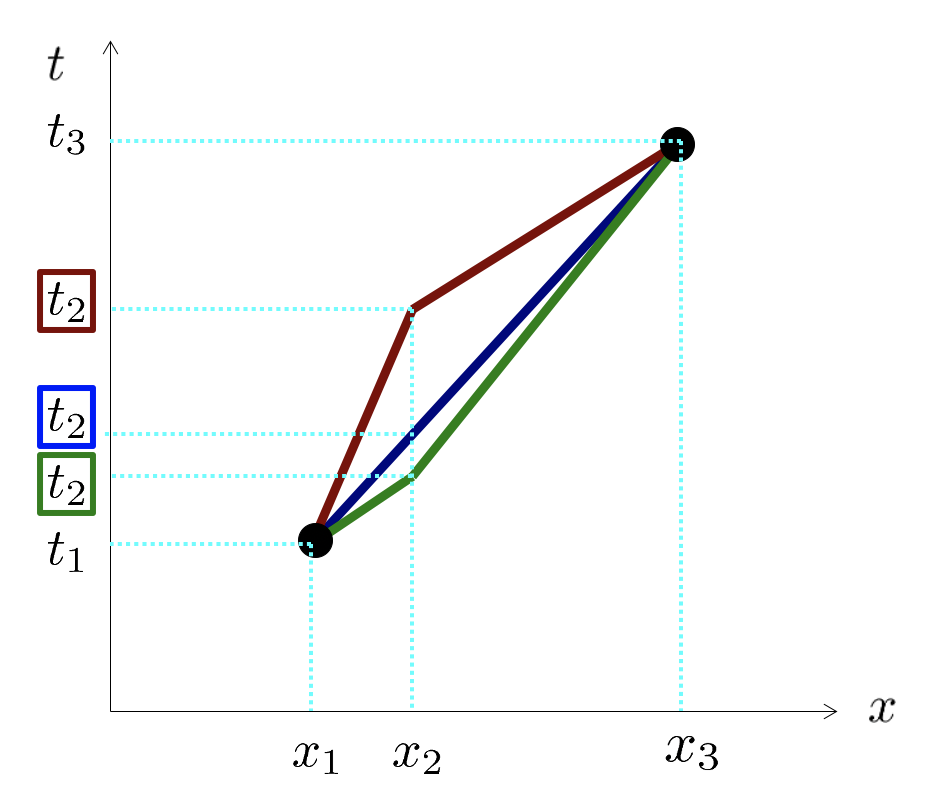
\includegraphics[scale=0.3]{media/maks_aldring1.png}}
Vi kaller nå avstanden fra $x_1$ til $x_2$ for $\Delta x_{12}$ og tidsintervallet mellom $t_1$ og $t_2$ for $\Delta t_{12}$. Tidromsintervallet fra punkt 1 til punkt 2 kaller vi $\Delta s_{12}$. Og helt tilsvarende for punkt 2 til 3 som vi kaller $\Delta x_{23}$, $\Delta t_{23}$ og $\Delta s_{23}$. {\bf Sett opp et uttrykk for den totale egentiden $\Delta\tau_{13}$ som ballen bruker fra punkt 1 til punkt 3 uttrykt kun ved  $\Delta x_{12}$, $\Delta t_{12}$,  $\Delta x_{23}$, $\Delta t_{23}$!}\textcolor{red}{Ikke gå videre før du har skrevet ned et forslag!}
}{SIDE 10/31/63}

\fullframenotxt{ma8}{ma7}{ma9}{0}{
\centerline{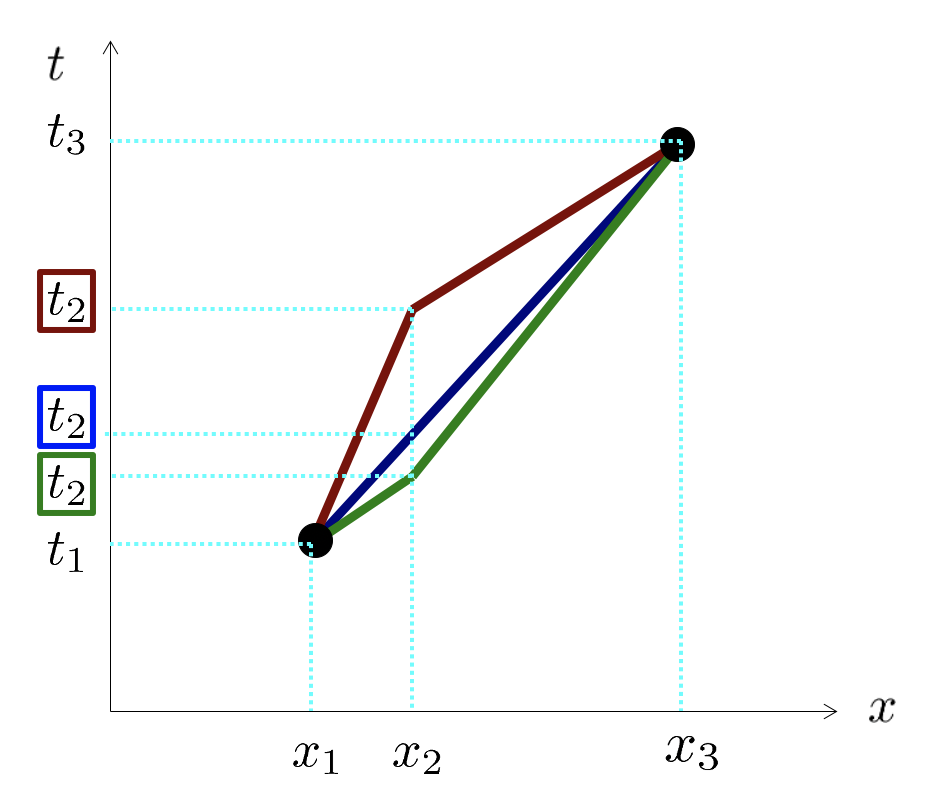
\includegraphics[scale=0.3]{media/maks_aldring1.png}}
Fikk du...\hyperlink{ma8_b}{\pagebutton{Ja, jeg fikk...}}\textcolor{white}{
\[
\Delta\tau_{13}=\sqrt{\Delta t_{12}^2-\Delta x_{12}^2}+\sqrt{\Delta t_{23}^2-\Delta x_{23}^2}
\]
Hvis du ikke ser hvordan du kommer frem til dette, ta en kikk på {denne videoen}.}
}{SIDE 11/31/63}

\fullframe{ma8_b}{ma7}{ma9}{0}{
\centerline{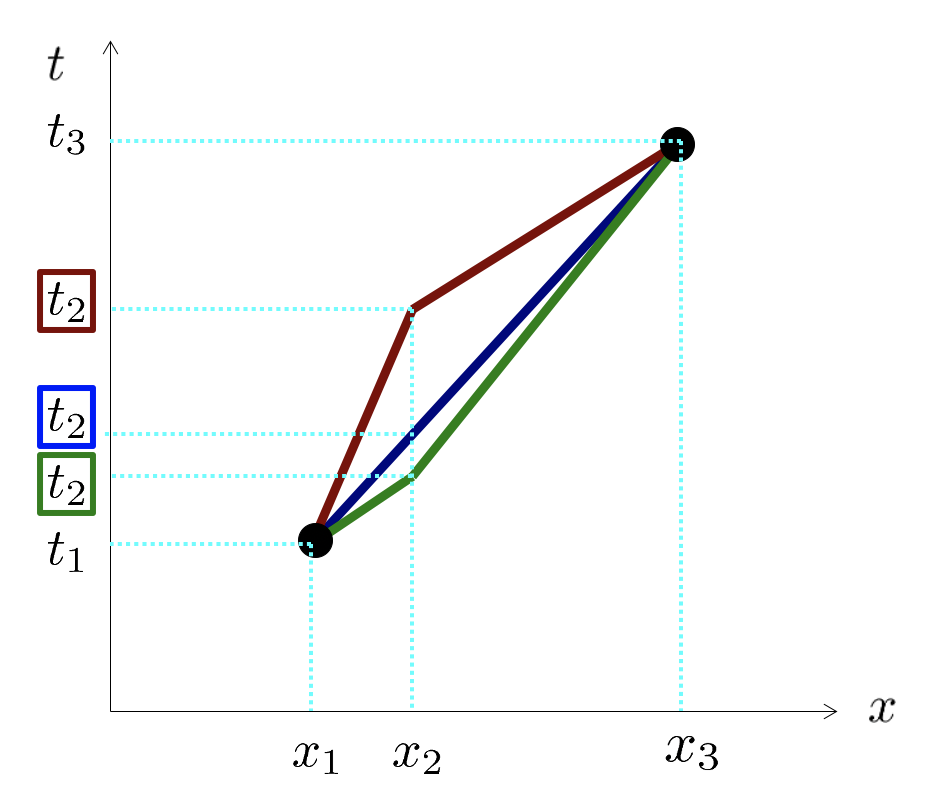
\includegraphics[scale=0.3]{media/maks_aldring1.png}}
Fikk du...{\pagebutton{Ja, jeg fikk...}}
\[
\Delta\tau_{13}=\sqrt{\Delta t_{12}^2-\Delta x_{12}^2}+\sqrt{\Delta t_{23}^2-\Delta x_{23}^2}
\]
Hvis du ikke ser hvordan du kommer frem til dette, ta en kikk på \href{https://www.uio.no/studier/emner/matnat/astro/AST2000/h20/undervisningsmateriell/interaktive-forelesningsnotater/2c/videoer/video2c_5.mp4}{denne videoen}.
}{SIDE 11/31/63}




\fullframe{ma9}{ma8}{ma10}{1}{
\centerline{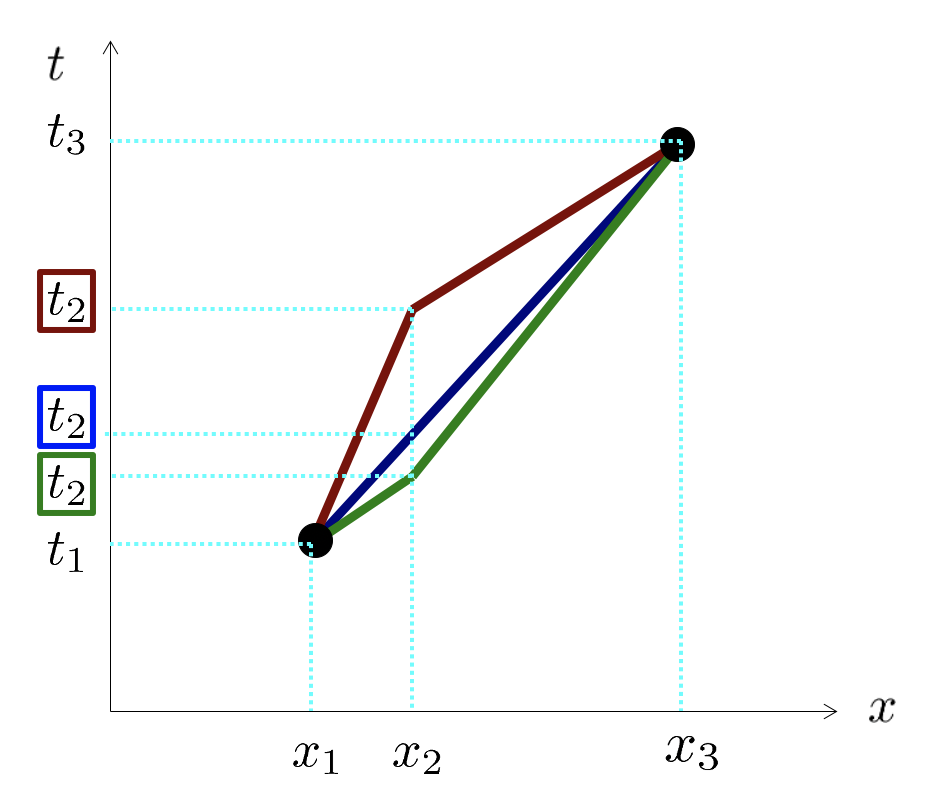
\includegraphics[scale=0.3]{media/maks_aldring1.png}}
Prinsippet om maksimal aldring sier oss av vi skal maksimalisere, altså finne maksimalpunktet for den totale egentiden $\Delta\tau_{13}$:
\[
\Delta\tau_{13}=\sqrt{\Delta t_{12}^2-\Delta x_{12}^2}+\sqrt{\Delta t_{23}^2-\Delta x_{23}^2}
\]
For å finne et ekstremalpunkt setter vi den deriverte lik null, men den deriverte med hensyn på {\bf hva?} Jo det må vel være med hensyn på $t_2$ som er vår ukjente. Vi skal altså finne den verdien for $t_2$ som gjør $\Delta\tau_{13}$ maksimal! {\bf MEEEN.....}
}{SIDE 12/31/63}

\fullframe{ma10}{ma9}{ma11}{0}{\small
\centerline{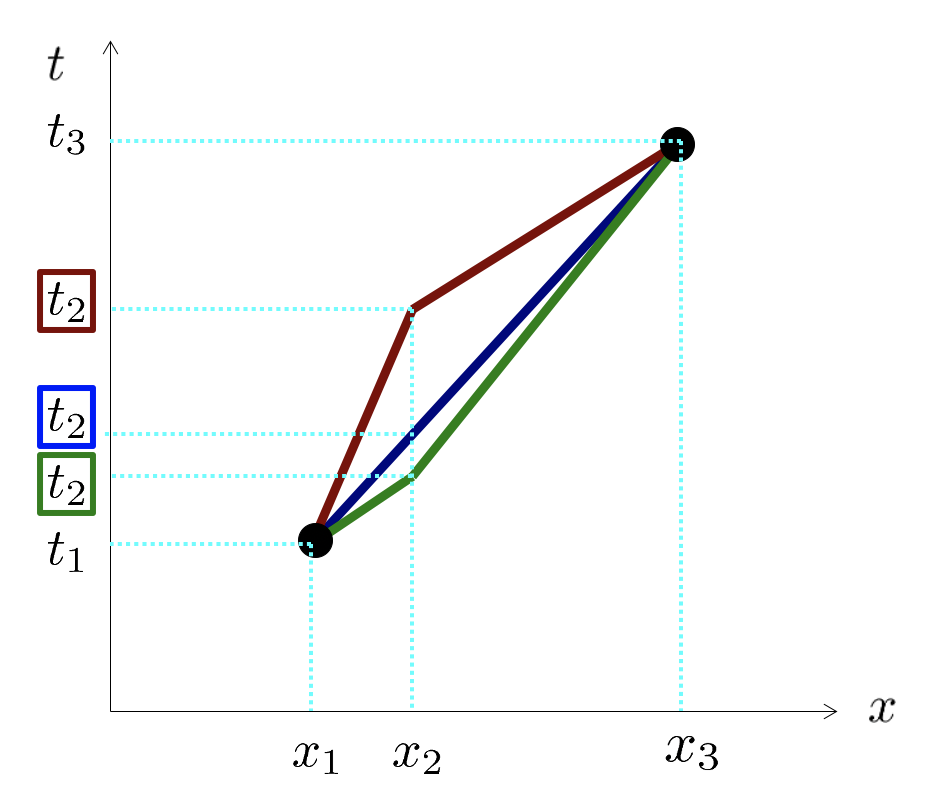
\includegraphics[scale=0.3]{media/maks_aldring1.png}}
\[
\Delta\tau_{13}=\sqrt{\Delta t_{12}^2-\Delta x_{12}^2}+\sqrt{\Delta t_{23}^2-\Delta x_{23}^2}
\]
{\bf ...det blir enklere å regne hvis vi isteden deriverer med hensyn på $\Delta t_{12}$, altså at vi prøver å finne den verdien for $\Delta t_{12}$ som maksimaliserer $\Delta\tau_{13}$.} $\Delta t_{12}$ er jo også en ukjent størrelse her siden $t_2$ er ukjent, og det er det samme hvilken ukjent størrelse vi bruker. Men kan du se hvordan vi kan skrive $\Delta t_{23}$ som jo inngår i uttrykket vår over uttrykt ved $\Delta t_{12}$ og $\Delta t_{13}$? (den siste er jo en {\bf kjent størrelse}). Og hvis du gjør det, kan du nå derivere og sette lik 0? Prøv selv først før du går videre...
}{SIDE 13/31/63}

\fullframenotxt{ma11}{ma10}{ma12}{0}{\small
\centerline{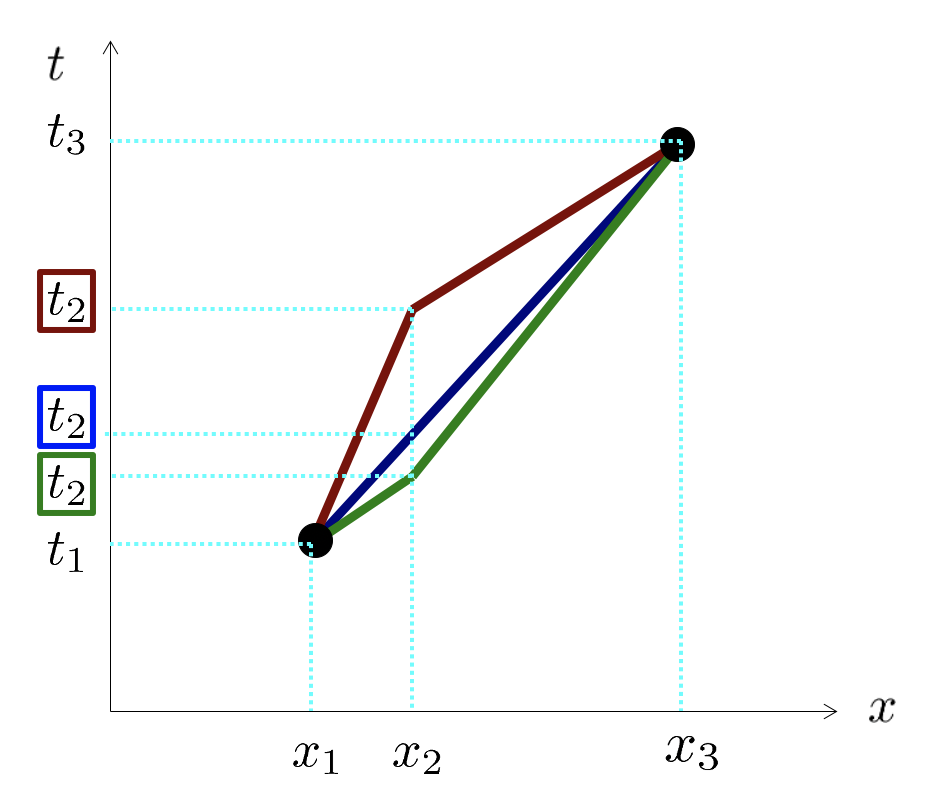
\includegraphics[scale=0.3]{media/maks_aldring1.png}}
Fikk du...\hyperlink{ma11_b}{\pagebutton{\small Ja, jeg fikk...}}\textcolor{white}{
\[
\frac{\Delta t_{12}}{\sqrt{\Delta t_{12}^2-\Delta x_{12}^2}}+\frac{\Delta t_{23}}{\sqrt{\Delta t_{23}^2-\Delta x_{23}^2}}=0
\]
??? Hvis du ikke fikk det til skal du snart se hvordan, men først, kan du se hvorfor du kan skrive dette som:
\[
\frac{\Delta t_{12}}{\Delta\tau_{12}}=\frac{\Delta _{23}}{\Delta\tau_{23}}
\]
({\bf Hint:} Hva er egentiden $\Delta\tau$ og hvordan kan du skrive den uttrykt med $\Delta t$ og $\Delta x$?)}
}{SIDE 14/31/63}

\fullframe{ma11_b}{ma10}{ma12}{0}{\small
\centerline{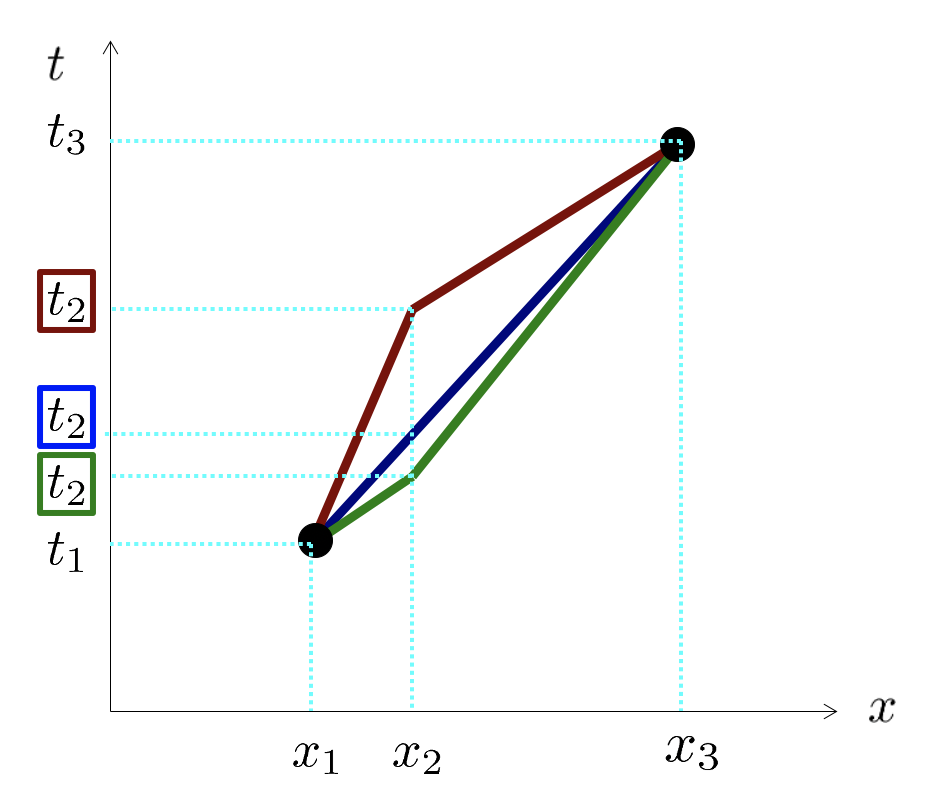
\includegraphics[scale=0.3]{media/maks_aldring1.png}}
Fikk du...{\pagebutton{\small Ja, jeg fikk...}}
\[
\frac{\Delta t_{12}}{\sqrt{\Delta t_{12}^2-\Delta x_{12}^2}}+\frac{\Delta t_{23}}{\sqrt{\Delta t_{23}^2-\Delta x_{23}^2}}=0
\]
??? Hvis du ikke fikk det til skal du snart se hvordan, men først, kan du se hvorfor du kan skrive dette som:
\[
\frac{\Delta t_{12}}{\Delta\tau_{12}}=\frac{\Delta _{23}}{\Delta\tau_{23}}
\]
({\bf Hint:} Hva er egentiden $\Delta\tau$ og hvordan kan du skrive den uttrykt med $\Delta t$ og $\Delta x$?)
}{SIDE 14/31/63}





\fullframe{ma12}{ma11}{ma13}{1}{\Large
\centerline{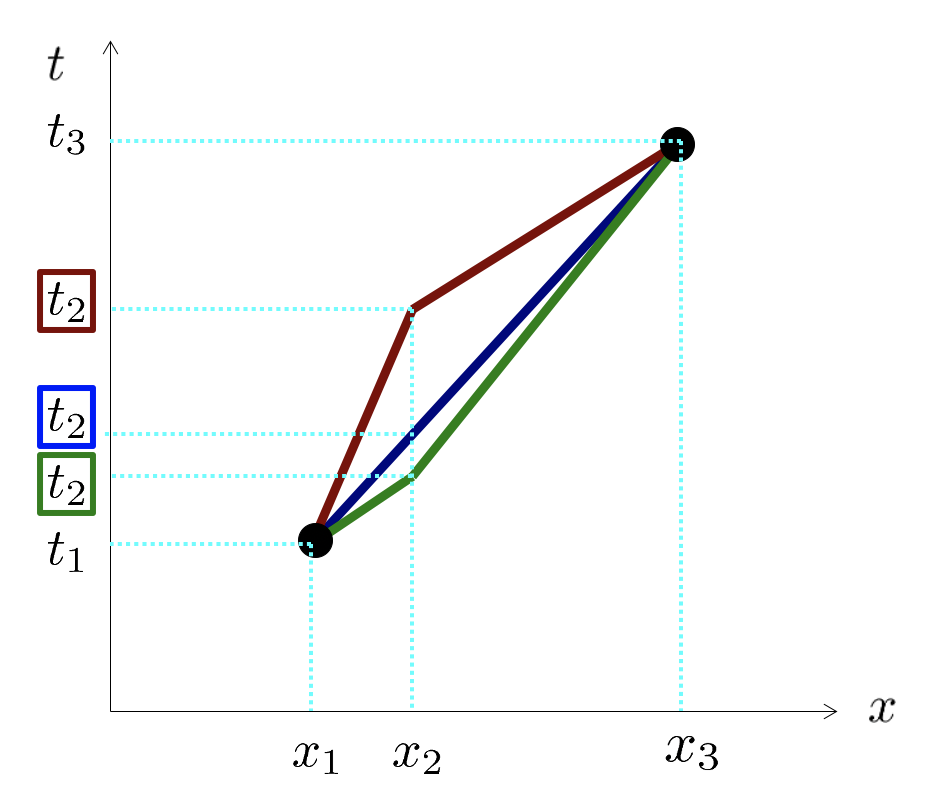
\includegraphics[scale=0.3]{media/maks_aldring1.png}}
Hvis du ikke klarte å komme frem selv, se på \href{https://www.uio.no/studier/emner/matnat/astro/AST2000/h20/undervisningsmateriell/interaktive-forelesningsnotater/2c/videoer/video2c_6.mp4}{denne videoen}.
}{SIDE 15/31/63}

\fullframe{ma13}{ma12}{ma14}{0}{
\centerline{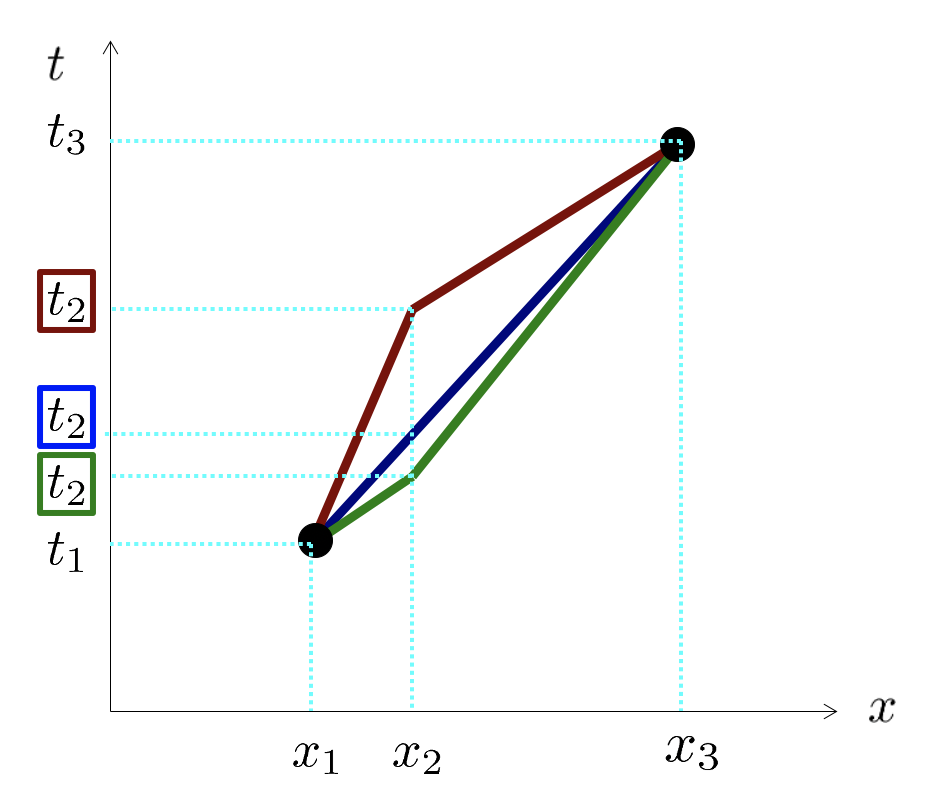
\includegraphics[scale=0.3]{media/maks_aldring1.png}}
Men hva står det egentlig her??? La oss ekstrapolere litt: Sett at du nå utvider verdenslinja med ett linjestykke til, et rett linje fra punkt 3 til punkt 4. Hvis vi nå gjentok denne utledningen fra punkt 2 til punkt 4 så vil vi jo {\bf nødvendigvis} helt tilsvarende finne:
\[
\frac{\Delta t_{23}}{\Delta\tau_{23}}=\frac{\Delta t_{34}}{\Delta\tau_{34}}
\]
Og slik fortsetter det utover verdenslinja. Det sier oss vel at vi har en bevart størrelse langs bevegelsen til ballen? Et uttrykk som generelt er bevart gjennom hele ballens bevegelse? {\bf Hvilket???}
}{SIDE 16/31/63}

\fullframetxt{ma14}{ma13}{ma15}{0}{DÆGGERN!!!! Jeg ser det!!!}{
\centerline{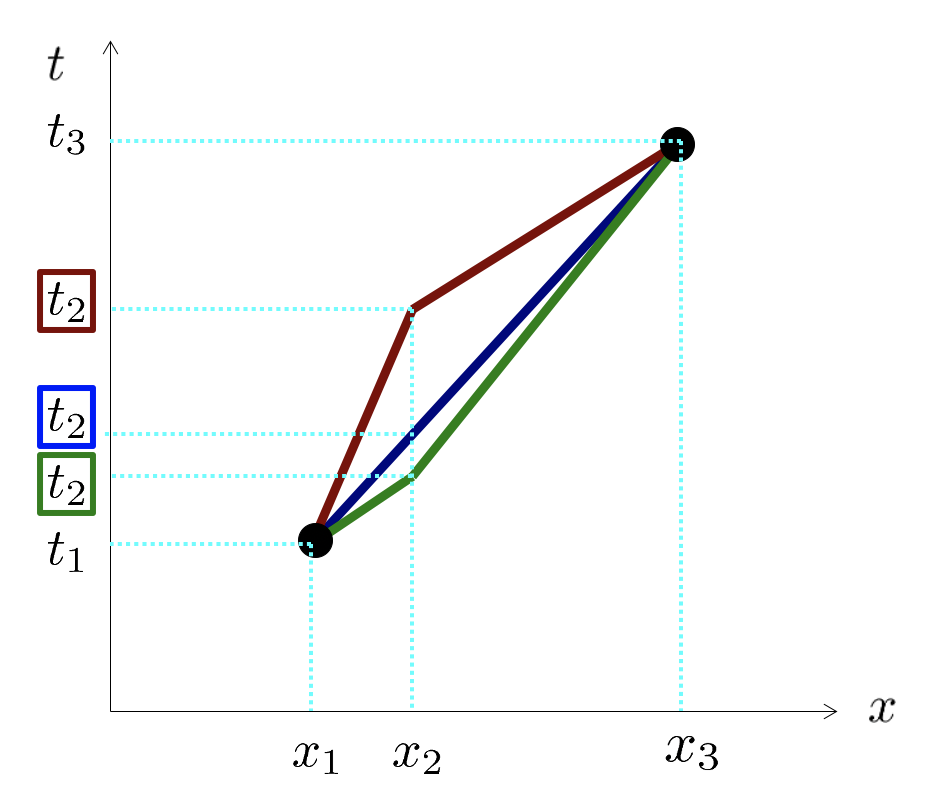
\includegraphics[scale=0.3]{media/maks_aldring1.png}}
Vi har jo funnet at
\[
\frac{\Delta t_{12}}{\Delta\tau_{12}}=\frac{\Delta t_{23}}{\Delta\tau t_{23}}=\frac{\Delta t_{34}}{\Delta\tau_{34}}
\]
dermed ser vi at størrelsen $\Delta t/\Delta\tau$ er bevart, enig? Men tenk på spesiell relativitetsteori, hvordan kan vi skrive en slik størrelse uttrykt med ballens hastighet? Tenk f.eks. at ballen er et tog, at $t$ er tiden målt fra bakken og $\tau$ jo er egentiden i toget...
}{SIDE 17/31/63}

\fullframe{ma15}{ma14}{red_ma16}{0}{
Er ikke $\Delta t/\Delta\tau$ bare forholdet mellom tiden i labsystemet og tiden i toget (ballen)??? Var ikke den
\[
\frac{\Delta t}{\Delta\tau}=\gamma
\]
??? Altså vi har utledet at $\gamma$ er en bevart størrelse!!! Men hvis $\gamma$ er bevart så betyr det at $v$ er bevart siden $\gamma=1/\sqrt{1-v^2}$!! Er ikke dette det vi ventet? {\bf Altså at vi har utledet at $v$ er den samme for alle linjestykker, altså konstant $v$ gjennom hele verdenslinja, Newtons første lov!} Men har vi utledet noe mer... hvilken annen størrelse avhenger av $\gamma$??
}{SIDE 18/31/63}

\colfullframe{red_ma16}{ma15}{ma17}{0}{red}{
\textcolor{yellow}{
Er ikke relativistisk energi gitt ved
\[
E=m\gamma
\]
??? Har vi utledet at energi per masse er en bevart størrelse? Altså $E/m$ er bevart? Kan se slik ut...\\
Kan altså være at prinsippet om maksimal aldring er det bakenforliggende prinsippet som sier oss hvorfor energi er en bevart størrelse?
{\bf (Merk at det er et punkt vi har hoppet over: vi har funnet ekstremalpunktet til $\Delta\tau_{13}$ men vi har ikke vist at dette er et maksimalpunkt! Det kan du gjøre ved å dobbeltderivere. Den øvelsen kan du gjøre selv hvis du ønsker, men tro meg, det er et maksimalpunkt!})
}
}{SIDE 19/31/63}

\fullframe{ma17}{red_ma16}{ma19}{0}{
\centerline{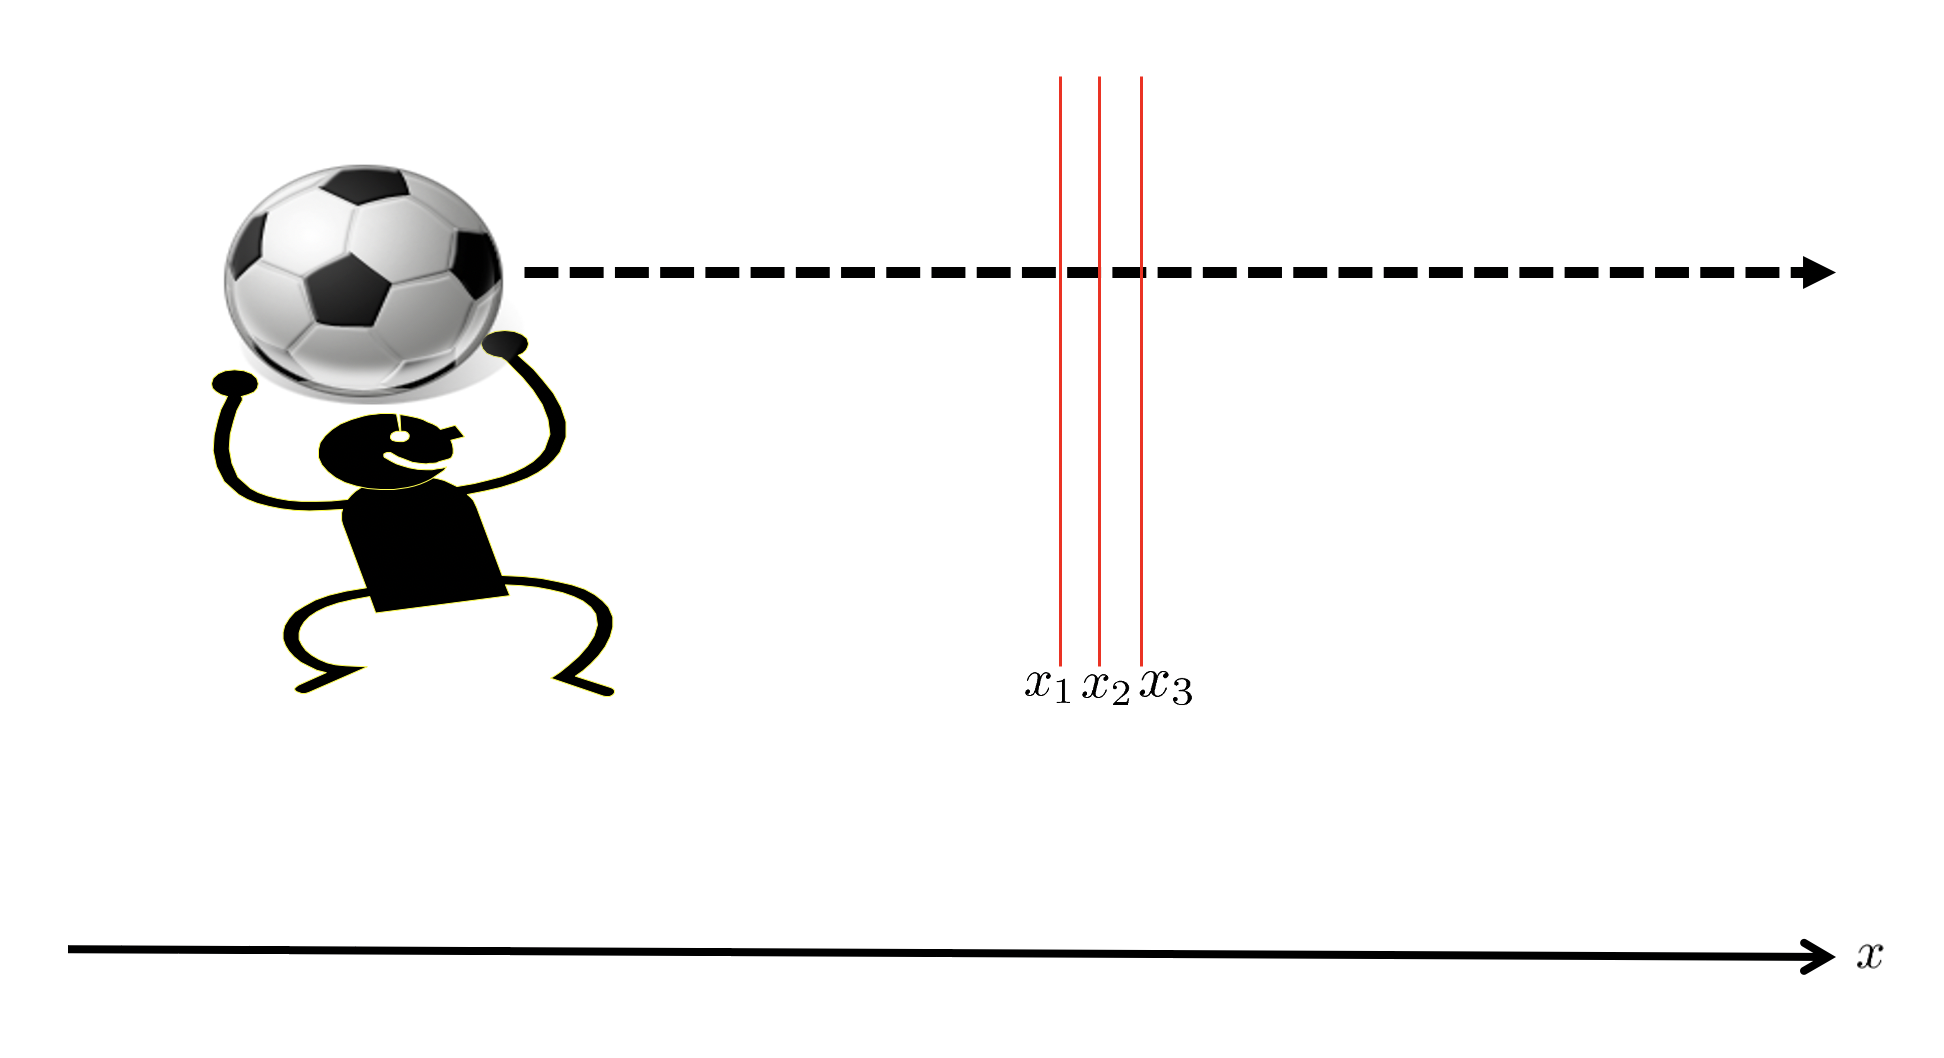
\includegraphics[scale=0.22]{media/maks_aldring2.png}}
Du skal nå helt på egenhånd få gjøre denne utledningen {\bf en gang til}! Men nå skal du anta at $t_2$ er kjent men $x_2$ er ukjent. Du skal altså maksimalisere egentiden  $\Delta\tau_{13}$ en gang til men nå med hensyn på $x_2$ eller da $\Delta x_{12}$. Vi skal se at vi da får et noe annet men minst like interessant resultat!
}{SIDE 20/31/63}

\fullframe{ma19}{ma17}{ma20}{0}{
\centerline{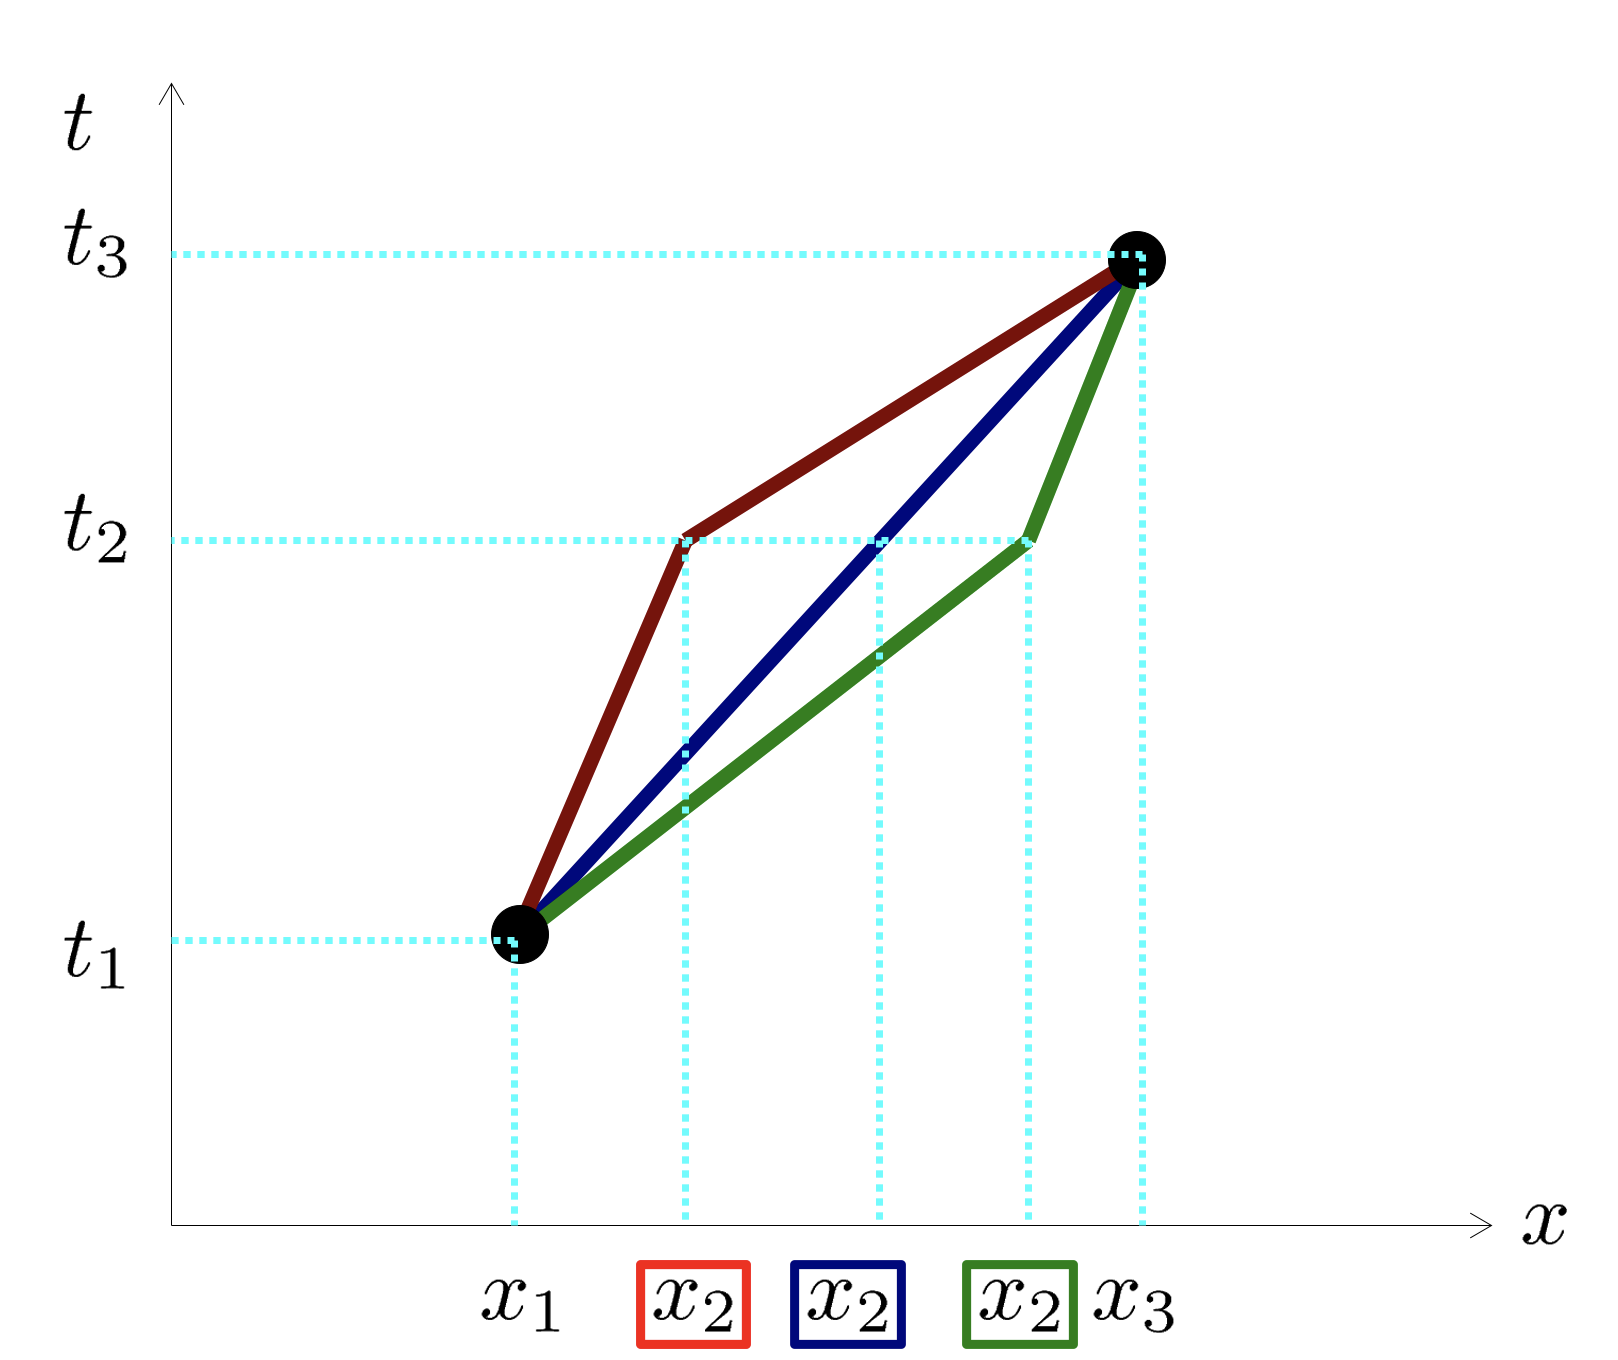
\includegraphics[scale=0.22]{media/maks_aldring3.png}}
Du får litt hjelp med denne figuren her. Men nå står du på egne ben! Merk at dere på prosjekt skal gjøre en slik utledning for et nytt tilfelle, og dette kan komme på eksamen, så det er viktig å få prøvd seg alene en gang. Og det vil hjelp på forståelsen for det som kommer, så dette er et godt øyeblikk å gjøre det på. Når du har gjort hele utledningen og funnet et størrelse som er bevart på samme måte som vi fant at $\gamma$ er bevart i forrige utledning, kan du bla om.
}{SIDE 21/31/63}


\fullframe{ma20}{ma19}{pause}{0}{\small
\centerline{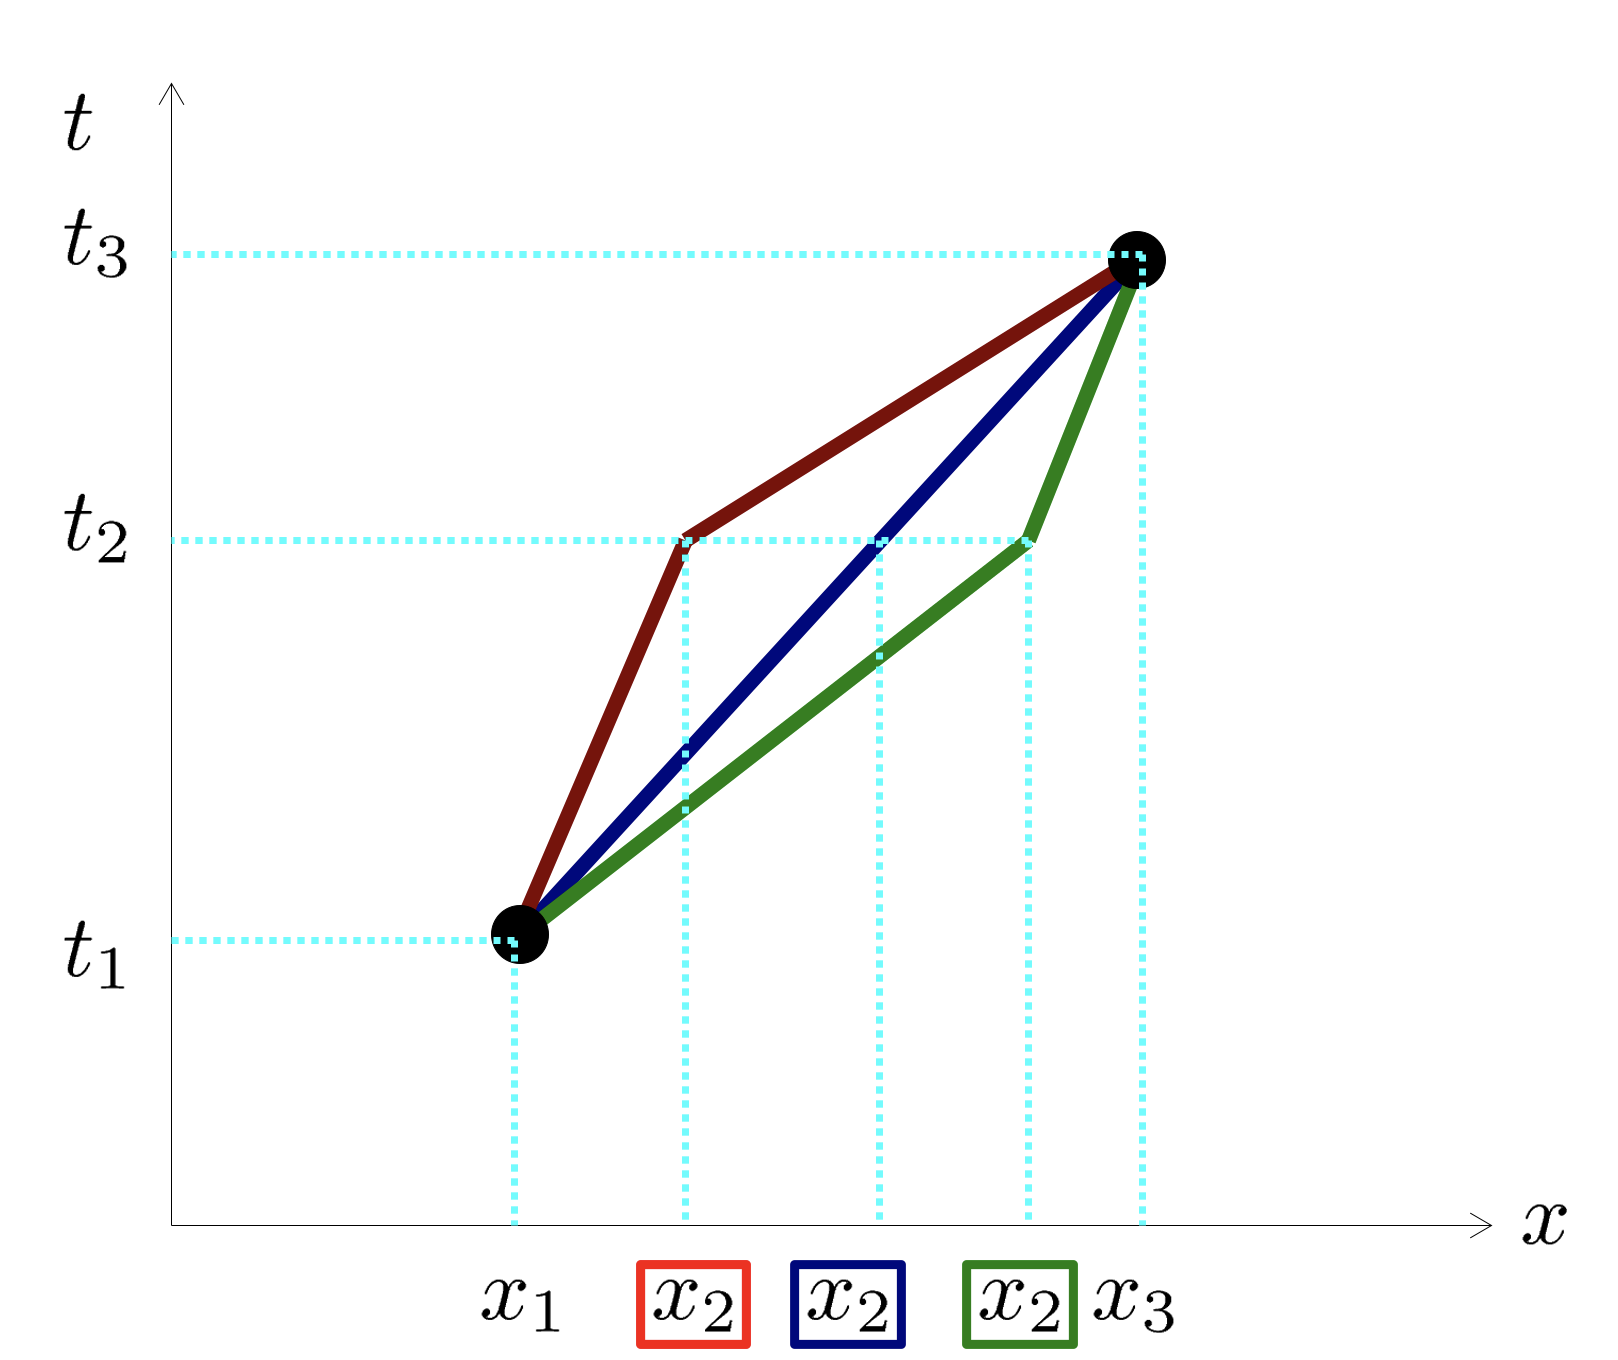
\includegraphics[scale=0.2]{media/maks_aldring3.png}}
{\bf Fikk du at $v\gamma$ er en bevart størrelse?} Hvis ikke, se gjennom utledningen i \href{https://www.uio.no/studier/emner/matnat/astro/AST2000/h20/undervisningsmateriell/interaktive-forelesningsnotater/2c/videoer/video2c_7.mp4}{denne videoen}!. Men vi vet jo at relativistisk bevegelsesmengde er gitt ved
\[
p=m\gamma v
\]
Har prinsippet om maksimal aldring her gitt oss bevaring av bevegelsesmengde? Eller det vil si, bevaring av bevegelsesmengde per masse $p/m$? Det er litt fristende å dra denne konklusjonen. Altså at prinsippet om maksimal aldring er et overliggende prinsipp som gir opphav til bevaring av energi og bevegelsesmengde. La oss se når vi setter på gravitasjon...
}{SIDE 22/31/63}

{
\setbeamercolor{background canvas}{bg=cyan}
\begin{frame}
\label{pause}
\hyperlink{ma20}{\pagebutton{\small Forrige side}}
{\huge
\centerline{Kaffe!}
\centerline{
\includegraphics[scale=4]{media/drink-coffee.png}}\\
}
\textcolor{yellow}{\large MEN først litt kaffe. Og etter kaffen, en tur ut, ta med deg ball. Kast den bortover og oppover og lim gjerne fast en klokke for å måle hvor mye ballen eldes. Og for å forberede deg på det neste: kast ballen rett oppover og se om den fortsetter med konstant hastighet eller om den akselereres på noen måte. Og hvis det siste skjer kan du jo filosofere litt rundt hvorfor den akselereres? Ikke gå videre før du {\bf er helt klar i hodet igjen!}}
\\
\vspace*{0.5cm}
\hyperlink{denim_ma21}{\pagebutton{Jeg er klar til å fortsette...}}
\end{frame}
}

\colfullframe{denim_ma21}{ma20}{red_ma21x}{0}{denim}{\footnotesize
\centerline{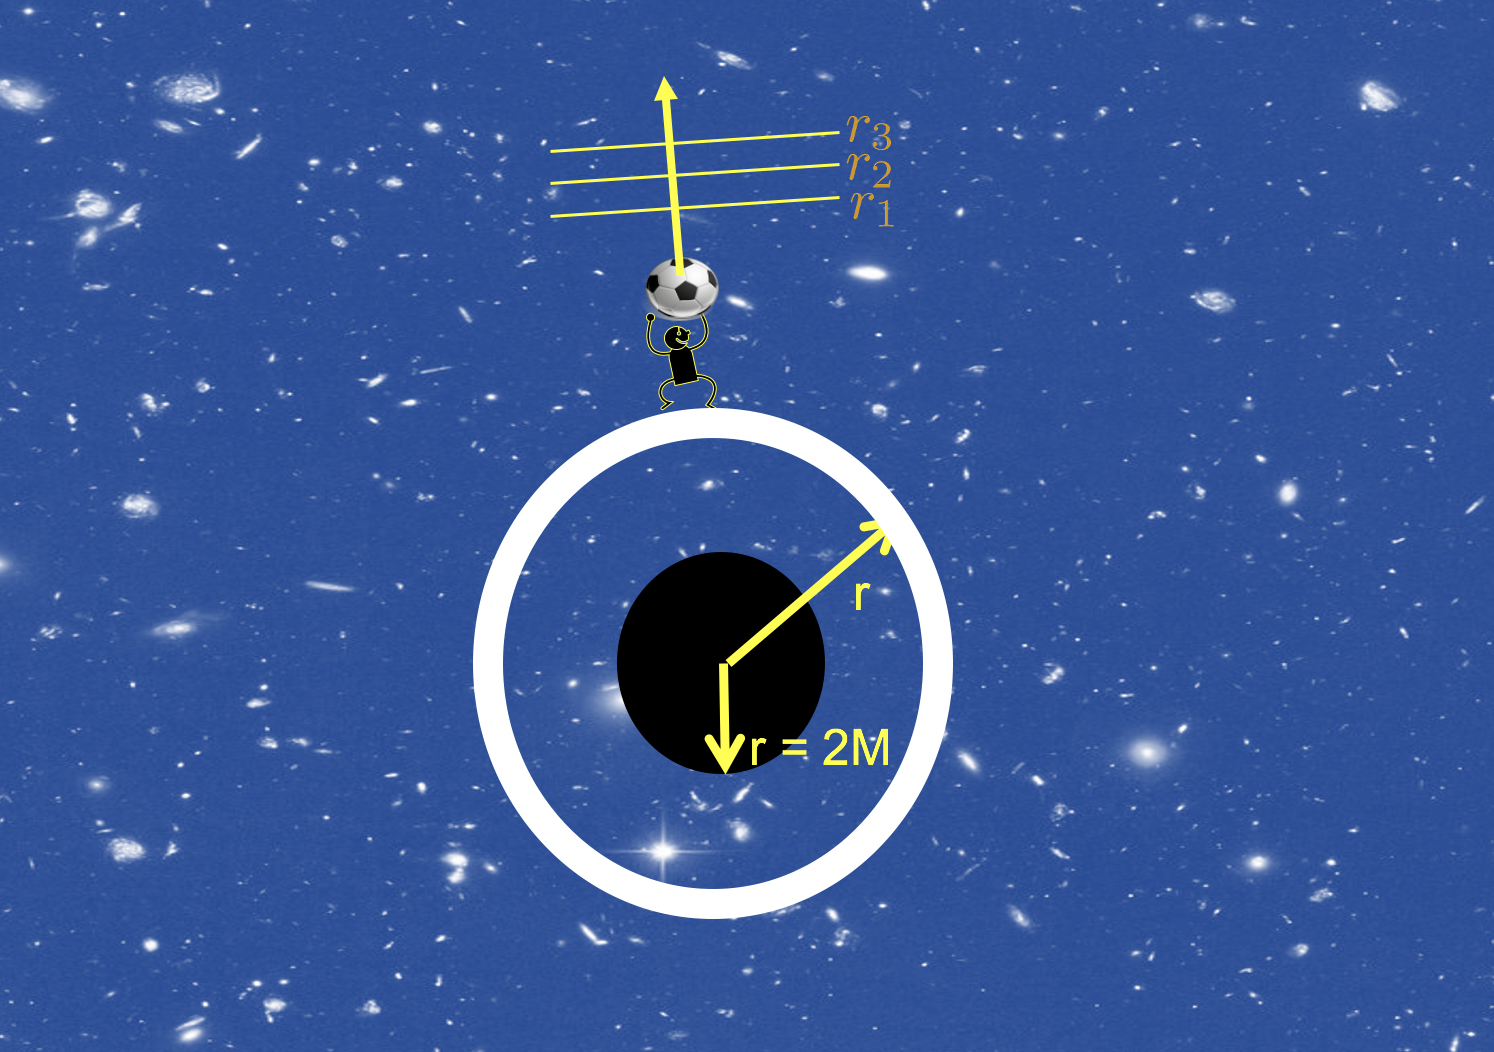
\includegraphics[scale=0.24]{media/maks_aldring4.png}}
\textcolor{yellow}{
Her ser vi situasjonen med gravitasjon. Skallobservatøren kaster en ball {\bf rett oppover i tyngdefeltet}. Ballen går altså oppover i $r$-retning og passerer punktene $r_1$, $r_2$ og $r_3$ på sin vei. {\bf Akkurat som for tilfellet med spesiell relativitetsteori så legger vi $r_1$ og $r_2$ så nær hverandre at ballen har konstant hastighet mellom disse to punktene. Helt tilsvarende mellom $r_2$ og $r_3$. Men farta $v_A$ mellom $r_1$ og $r_2$ trenger ikke å være den samme som farta $v_B$ mellom  $r_2$ og $r_3$.} Vi skal også se at vi trenger å definere avstanden $r_A$ som er midlet av avstanden mellom $r_1$ og $r_2$, altså i praksis midtpunktet mellom de to. Helt tilsvarende er $r_B$ midtpunktet mellom $r_2$ og $r_3$. Vi skal nå bruke prinsippet om maksimal aldring til å finne ballens rette verdenslinje...
}
}{SIDE 23/31/63}

\colfullframe{red_ma21x}{denim_ma21}{ma22}{0}{red}{\large
\textcolor{yellow}{
Men stopp en hal! Husker du at prinsippet om maksimal aldring {\bf kun gjelder legemer som er i fri flyt?} Altså legemer som det ikke virker noen krefter på!!! {\bf VEL, i generell relativitetsteori er ikke gravitasjonen regnet som en kraft!} Som vi skal se så er det krumningen av tidrommet som gir seg utslag i noe som ser ut som en kraft. Men ifølge relativitetsteorien så {\bf er det ingen kraft}. Dermed er et legeme under gravitasjonspåvirkning enda i fri flyt. Og det er geometrien til tidrommet kombinert med prinsippet om maksimal aldring som gir opphav til akselrasjon, {\bf ikke noen kraft!}
}
}{SIDE 24/31/63}

\fullframe{ma22}{red_ma21x}{ma23}{0}{\small
\centerline{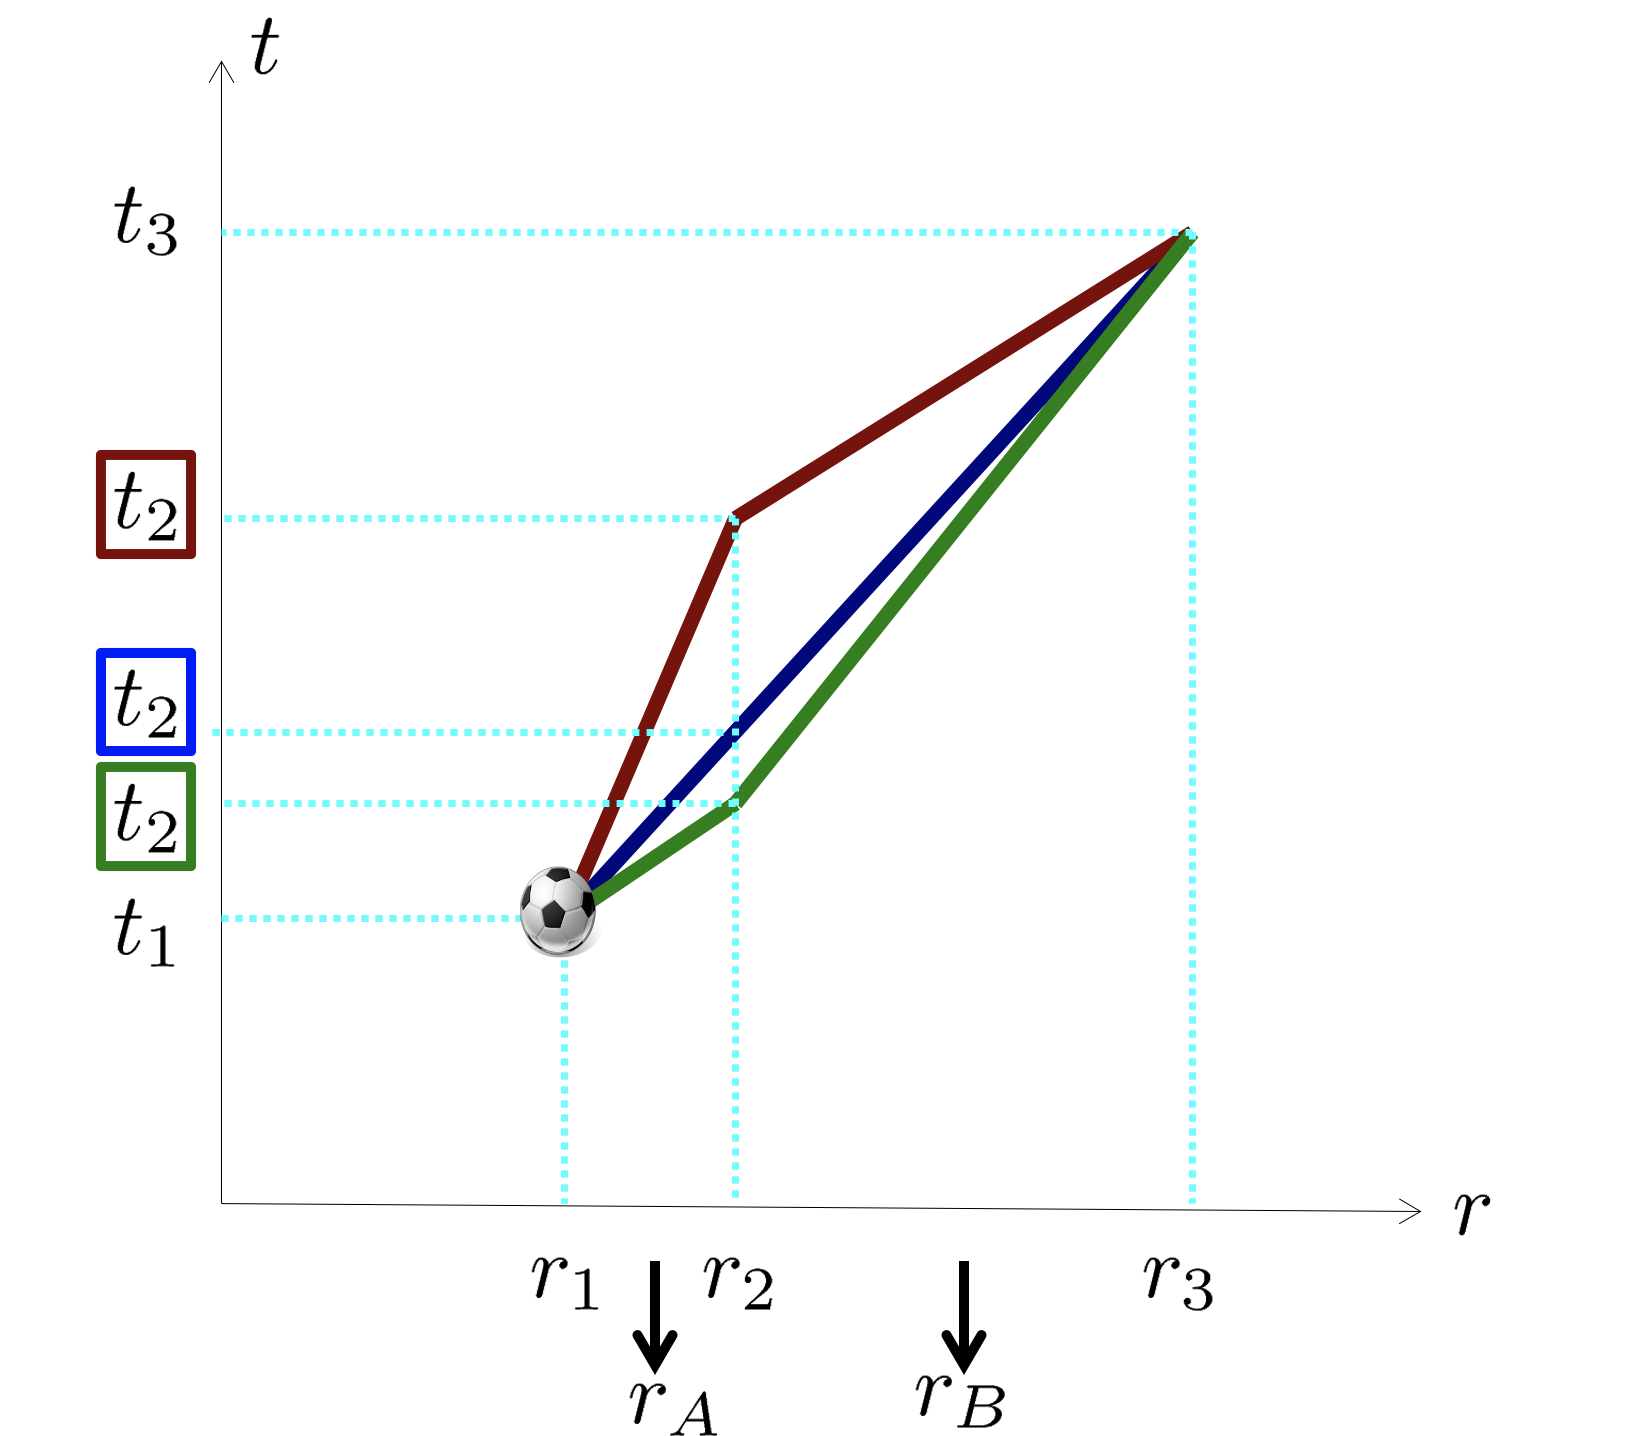
\includegraphics[scale=0.2]{media/maks_aldring5.png}}
Her ser vi igjen 3 mulige verdenslinjer, eller rettere sagt det bittelille utsnittet av mulige verdenslinjer til ballen mellom høyde $r_1$ til $r_3$ fra tidspunkt $t_1$ til $t_3$ der det har konstant hastighet (rett linje) fra $r_1$ til $r_2$ og en (mulig) annen konstant hastighet fra $r_2$ til $r_3$. Her beveger ballen seg over flere skall så vi kan ikke anta lokalt inertialsystem for hele reisen. Dermed må vi bruke \ss-geometri. Kan du sette opp et uttrykk for den totale egentida slik som du gjorde tidligere? Ikke bla om før du har et forslag.
}{SIDE 25/31/63}

\fullframetwo{ma23}{ma22}{ma24}{0}{
\centerline{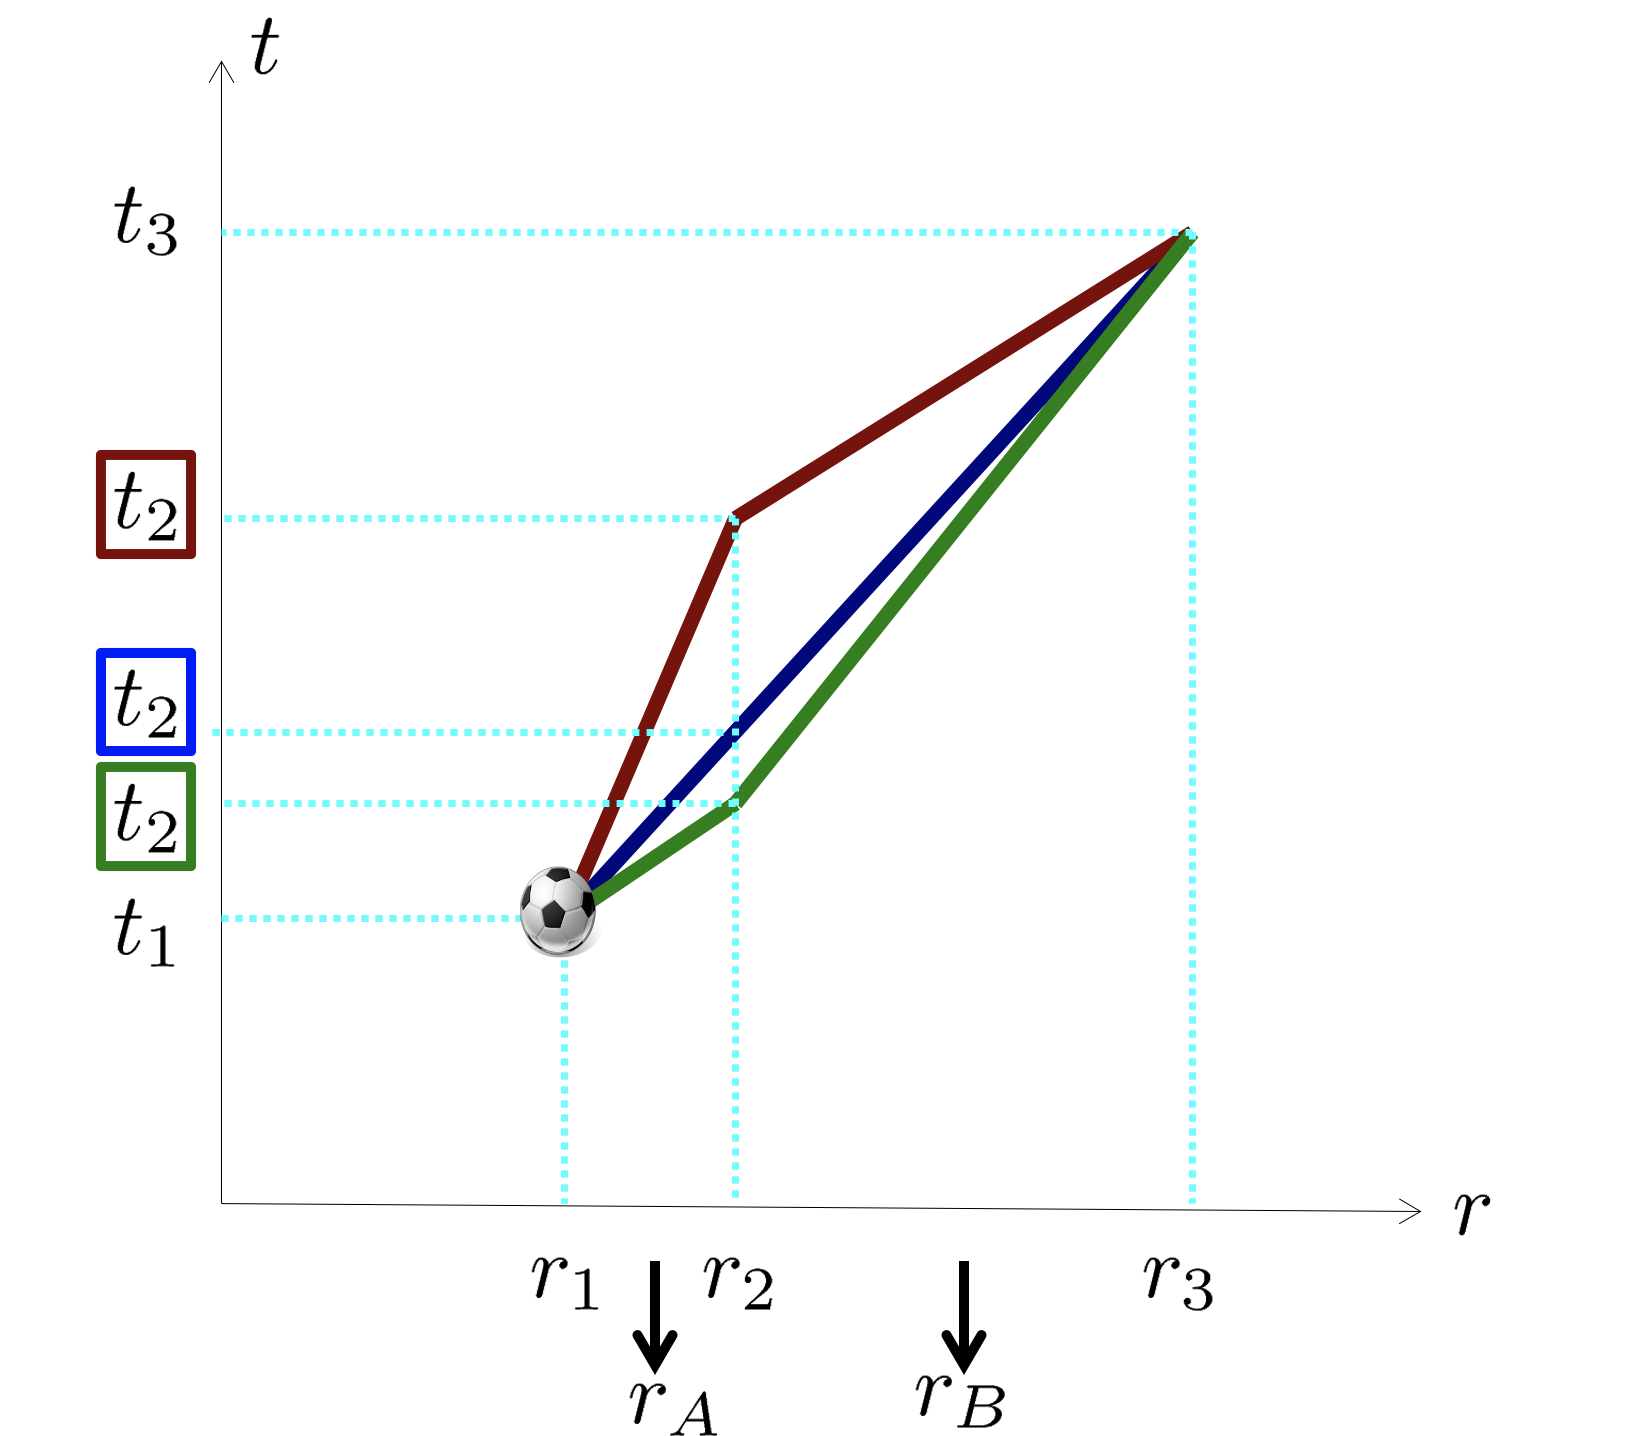
\includegraphics[scale=0.22]{media/maks_aldring5.png}}}
{\footnotesize
Fikk du:
\begin{align*}
\Delta\tau_{13}&=\Delta\tau_{12}+\Delta\tau_{23} \\
&=\sqrt{\left(1-\frac{2M}{r_A}\right)\Delta t_{12}^2-\frac{\Delta r_{12}^2}{\left(1-\frac{2M}{r_A}\right)}} \\
& \qquad +\sqrt{\left(1-\frac{2M}{r_B}\right)\Delta t_{23}^2-\frac{\Delta r_{23}^2}{\left(1-\frac{2M}{r_B}\right)}},
\end{align*}
Ser du nå hvorfor vi trenger $r_A$ og $r_B$? Hvis ikke se \href{https://www.uio.no/studier/emner/matnat/astro/AST2000/h20/undervisningsmateriell/interaktive-forelesningsnotater/2c/videoer/video2c_8.mp4}{se denne videoen} for utledning og forklaringer. {\bf Vi skal nå bruke prinsippet om maksimal aldring på denne egentiden $\Delta\tau_{13}$ og finne hvilket tidspunkt $t_2$, og dermed hvilken verdenslinje, som maksimaliserer egentida.}
}{SIDE 26/31/63}

\fullframetwo{ma24}{ma23}{ma25}{0}{
\centerline{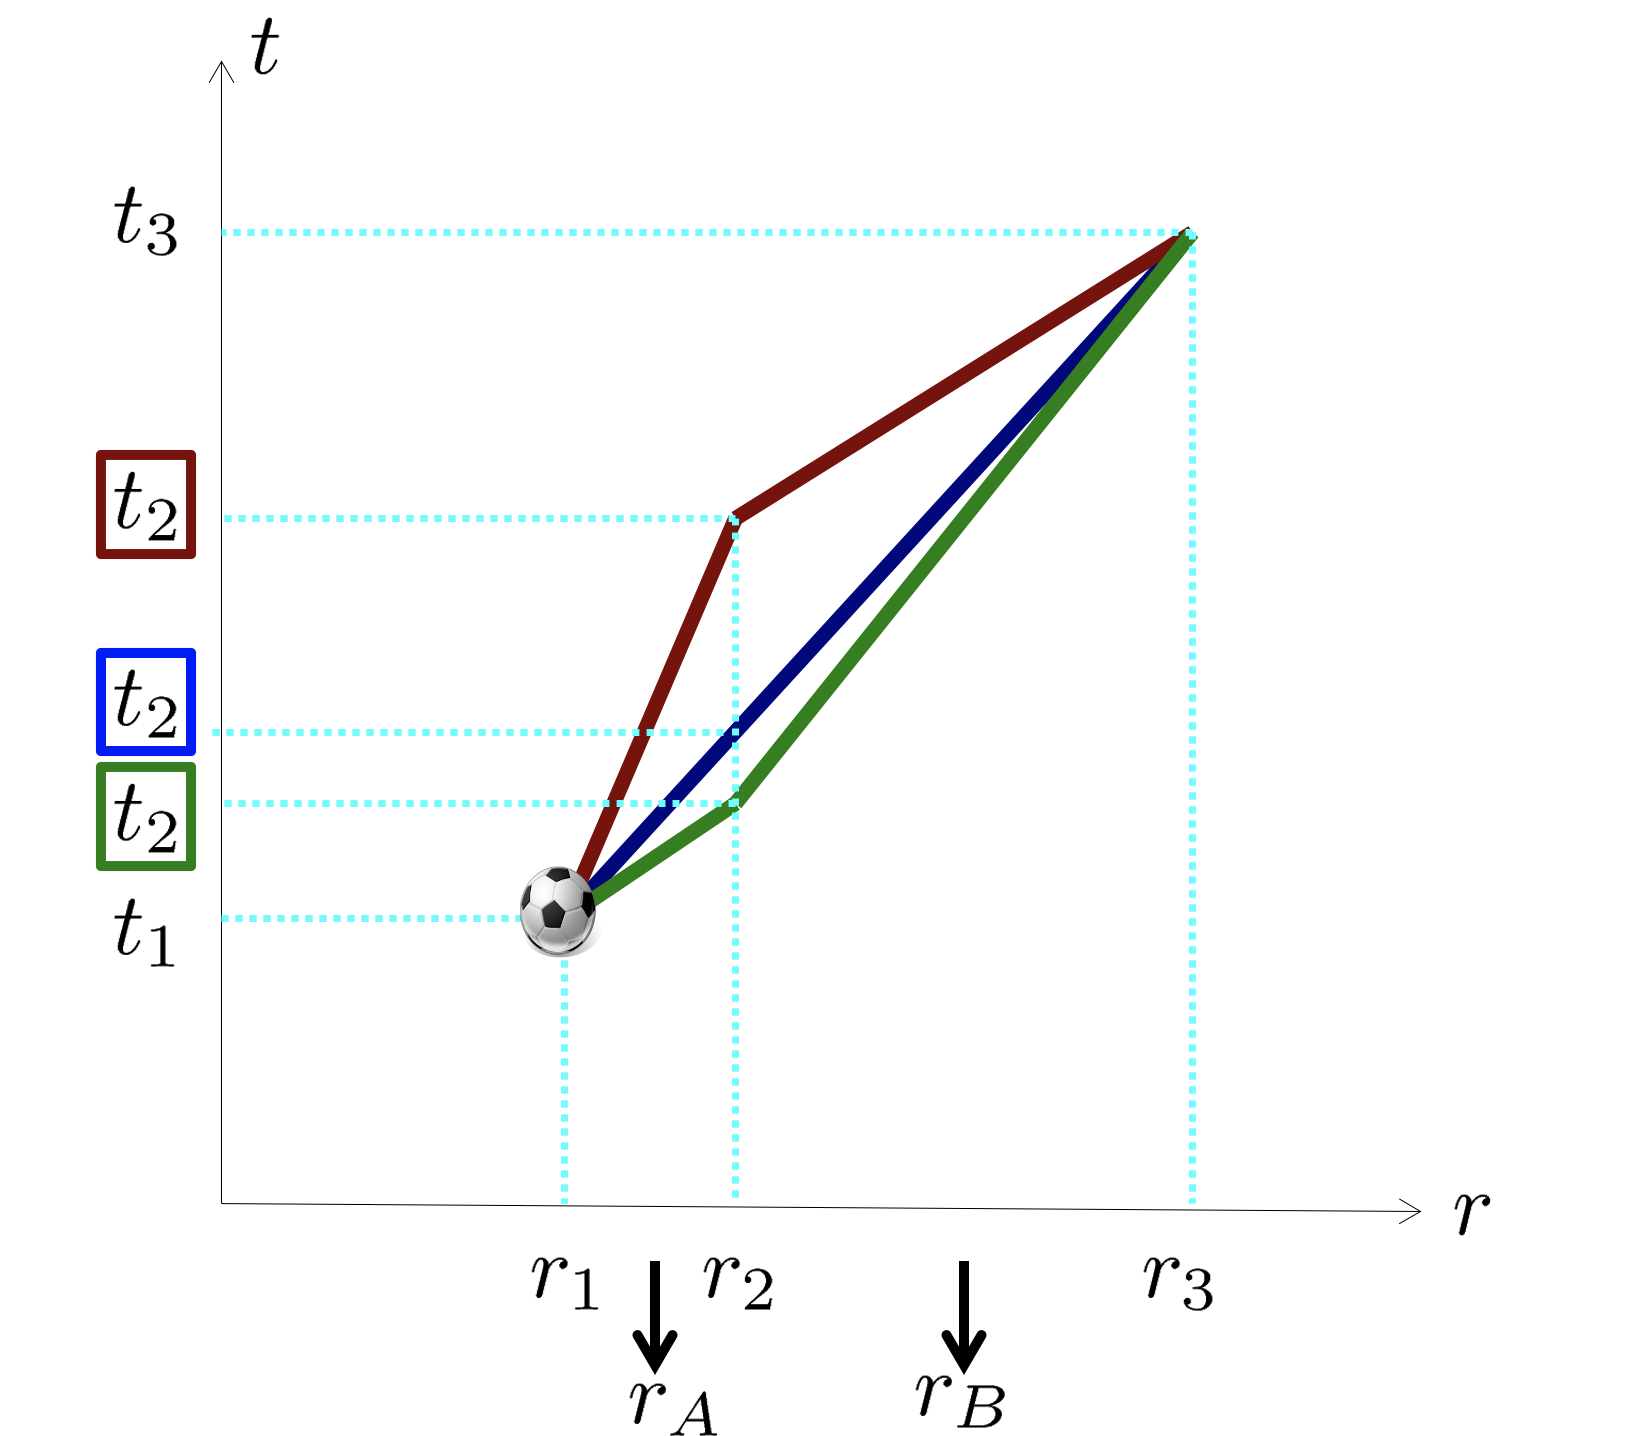
\includegraphics[scale=0.22]{media/maks_aldring5.png}}}
{\footnotesize
Hvis du som før deriverer dette med hensyn på $\Delta t_{12}$, setter dette lik 0 og setter inn for egentidene $\Delta\tau_{12}$ og  $\Delta\tau_{23}$  akkurat som før får du da:
\[
\frac{\left(1-\frac{2M}{r_A}\right)\Delta t_{12}}{\Delta\tau_{12}}=\frac{\left(1-\frac{2M}{r_B}\right)\Delta t_{23}}{\Delta\tau_{23}}.
\]
{\bf Hvis ikke, se \href{https://www.uio.no/studier/emner/matnat/astro/AST2000/h20/undervisningsmateriell/interaktive-forelesningsnotater/2c/videoer/video2c_9.mp4}{denne videoen for detaljer}}. \textcolor{red}{Ser du også her, på samme måte som for eksemplene med Lorentzgeometri, at vi har funnet en størrelse som er bevart langs verdenslina? {\bf Hva er denne størrelsen?}}
}{SIDE 27/31/63}

\fullframetwo{ma25}{ma24}{ma26}{0}{
\centerline{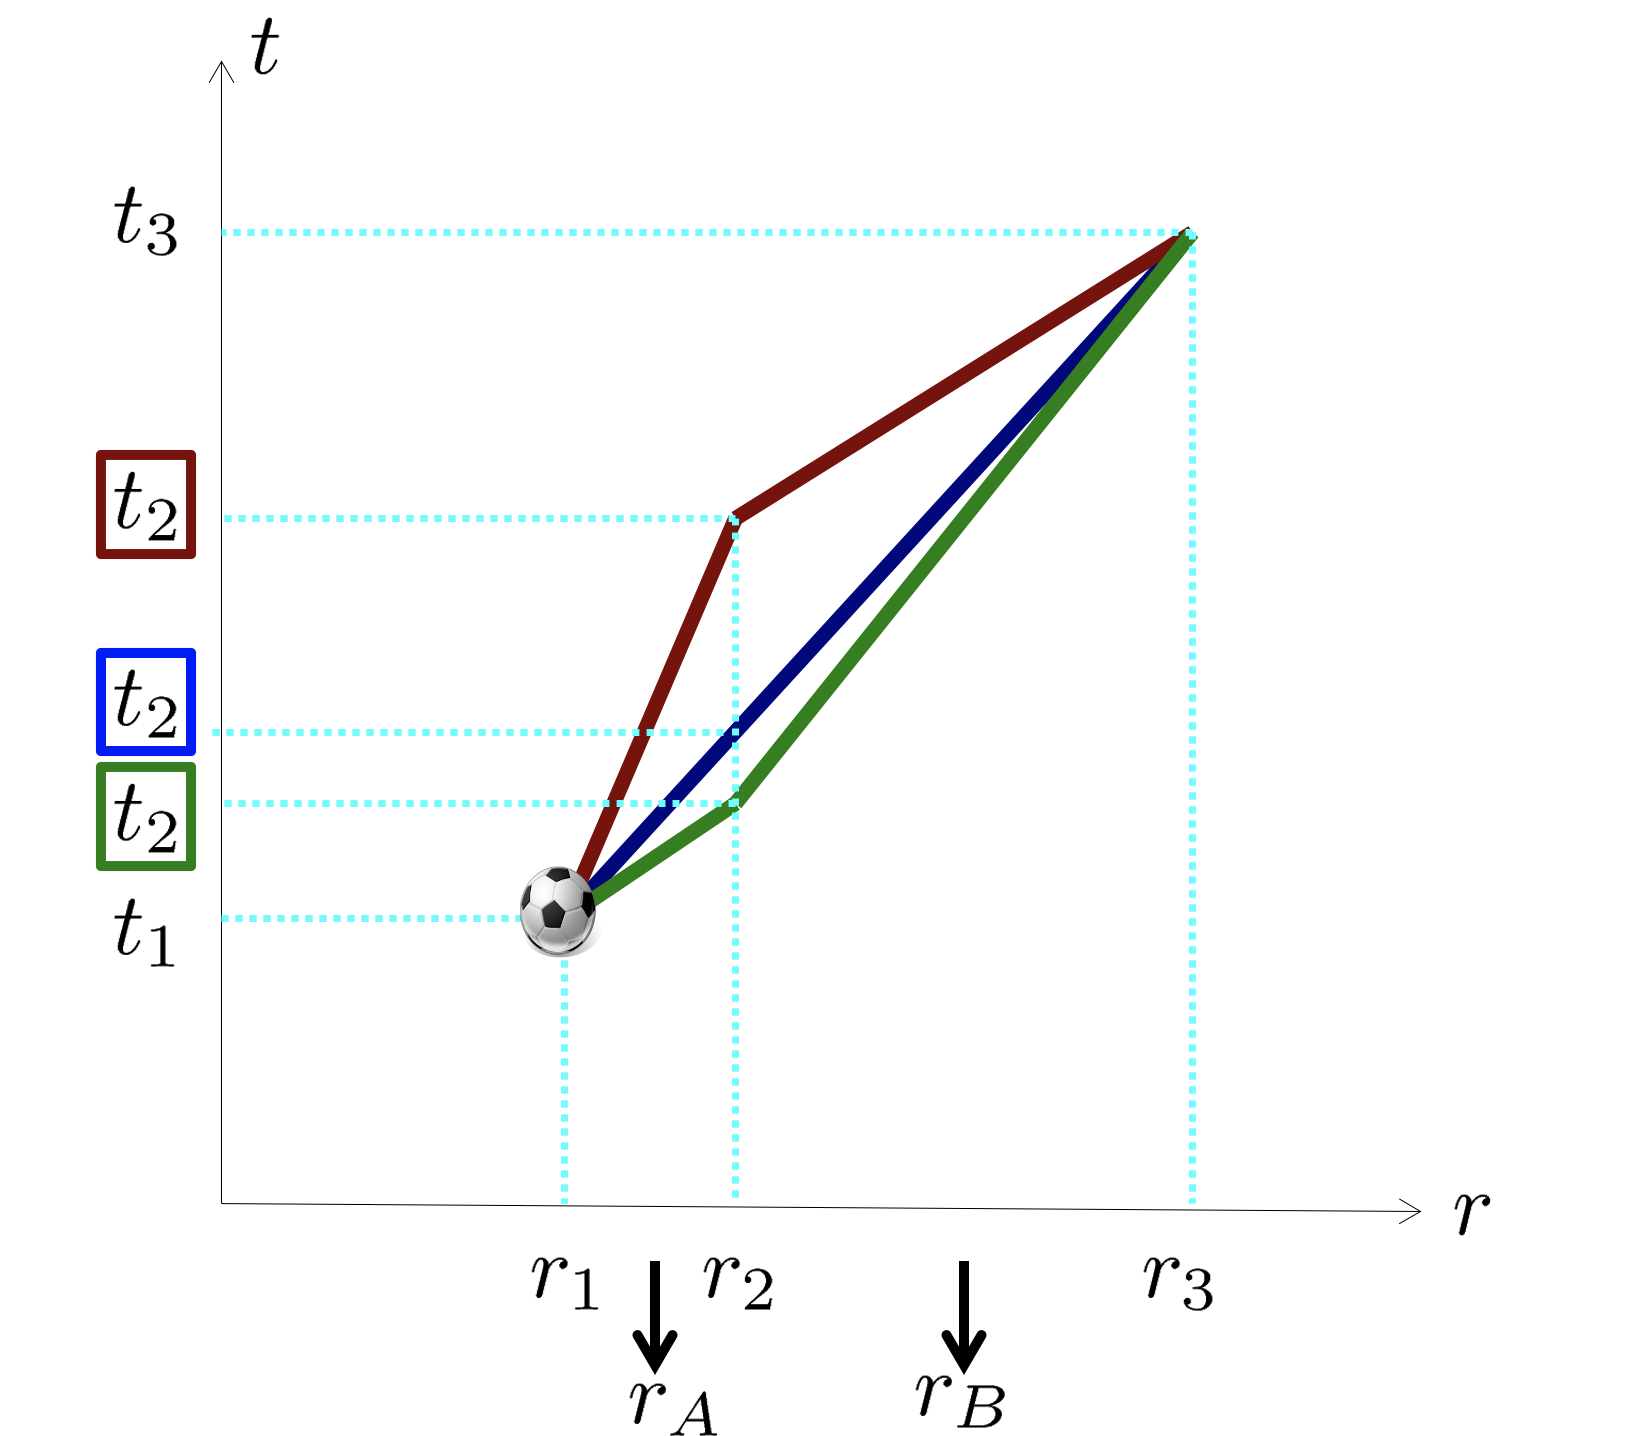
\includegraphics[scale=0.22]{media/maks_aldring5.png}}}
{\footnotesize
Fikk du at størrelsen
\[
\left(1-\frac{2M}{r}\right)\frac{\Delta t}{\Delta\tau}
\]
er en størrelse som er bevart langs (ved ekstrapolasjon) hele bevegelsen til ballen?
{\bf Men hva i allverden sier dette oss for noe?} I \href{https://www.uio.no/studier/emner/matnat/astro/AST2000/h20/undervisningsmateriell/interaktive-forelesningsnotater/2c/videoer/video2c_10a.mp4}{denne videoen} skriver vi om og tolker uttrykket.
}{SIDE 28/31/63}


\fullframetwo{ma26}{ma25}{ma27}{0}{
\centerline{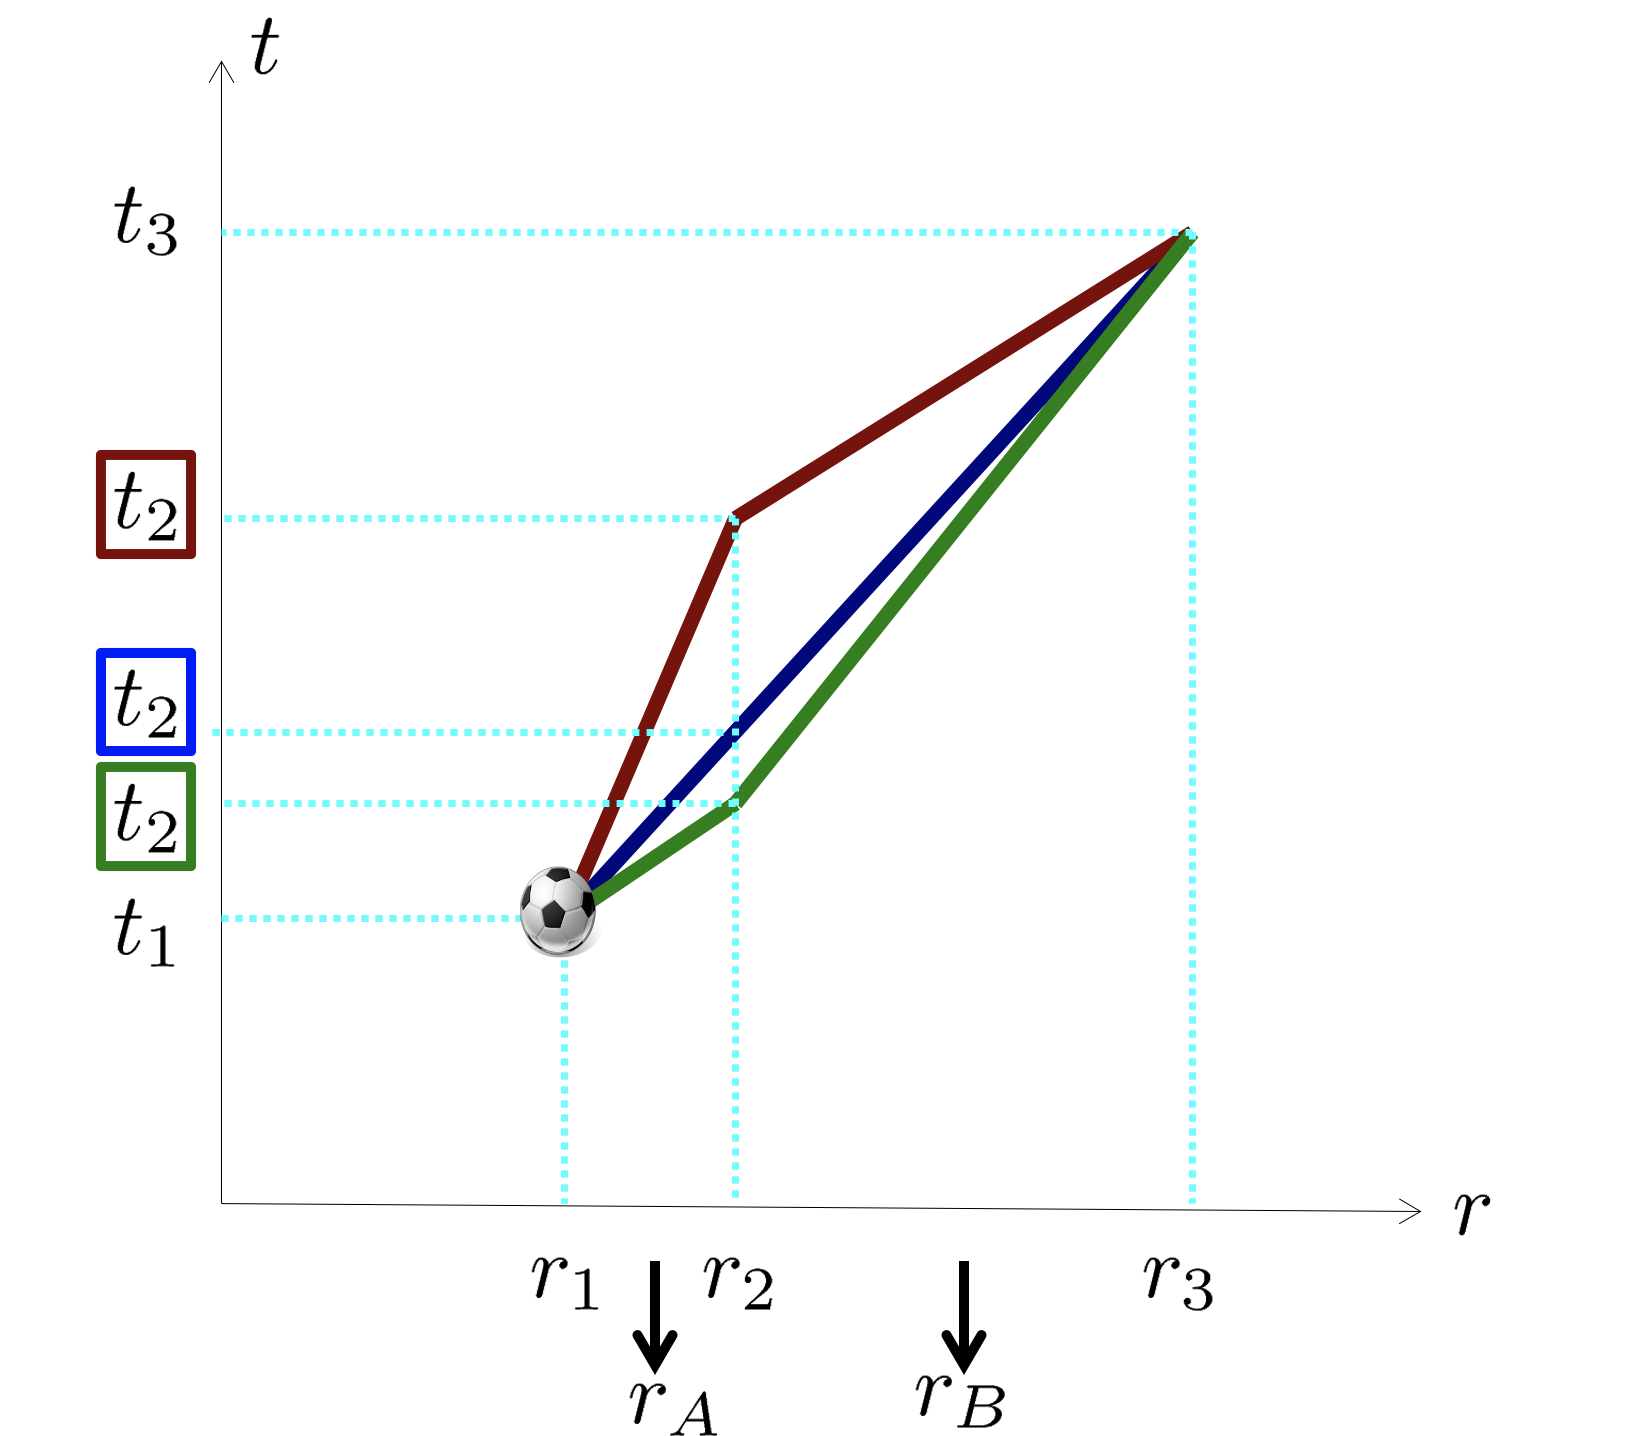
\includegraphics[scale=0.21]{media/maks_aldring5.png}}
\footnotesize
I videoen ser vi at uttrykket som er bevart
\[
\left(1-\frac{2M}{r}\right)\frac{\Delta t}{\Delta\tau}
\]
kan skrives som
\[
\sqrt{1-\frac{2M}{r}}\frac{1}{\sqrt{1-v_\mathrm{sh}^2}}
\]
}
{\footnotesize
der $v_\mathrm{sh}$ er farta målt av en skallobservatør som er {\bf på akkurat det skallet som ballen er i et gitt øyeblikk.}
\textcolor{red}{Vi ser at denne størrelsen forteller oss at ballen sakker farten sin når den er på vei oppover i tyngdefeltet:} Hvis dette skal være en bevart størrelse, og hvis $r$ øker (ballen beveger seg oppover), {\bf ja da må $v_\mathrm{sh}$ minke} for å bevare denne størrelsen! {\bf Ser du det?}\\

{\bf Men hva i allverden er dette for en størrelse?} Som vi så i del 2B så er et typisk triks for å tolke relativistiske størrelser å gå til grensen med lave hastigheter og {\bf i dette tilfellet også svake gravitasjonsfelt.} Ved svake gravitasjonsfelt, altså langt fra sorte hull bør vi få tilbake noe Newtonsk. I \href{https://www.uio.no/studier/emner/matnat/astro/AST2000/h20/undervisningsmateriell/interaktive-forelesningsnotater/2c/videoer/video2c_10b.mp4}{denne videoen} rekkeutvikler vi og tolker uttrykket.
}{SIDE 29/31/63}


\fullframe{ma27}{ma26}{ma28}{0}{\large
I videoen så vi at den bevarte størrelsen vår tilsvarer total energi per masse til ballen, hvileenergi, kinetisk energi og potensiell gravitasjonsenergi i et og samme uttrykk:
\[
\frac{E}{m}=\sqrt{1-\frac{2M}{r}}\frac{1}{\sqrt{1-v_\mathrm{sh}^2}}\approx1+\frac{1}{2}v^2-\frac{M}{r}
\]
der tilnærmelsen gjelder for lave hastigheter $v<<1$ og svake gravitasjonsfelt $r>>M$, det vi kaller for {\bf den klassiske grensen}. Ganger vi opp med $m$ og bruker SI-enheter ser vi at vi får
\[
E\approx mc^2+\frac{1}{2}mv^2-G\frac{Mm}{r}
\]
i den klassiske grensen.
}{SIDE 30/31/63}

\fullframe{ma28}{ma27}{blue_nytema2}{0}{
Vi har altså
\begin{block}{det generelle uttrykket for energi per masse til et legeme...}
...med masse $m$ i tyngdefeltet til en kulesymmetrisk massefordeling med masse $M$ i en koordinatavstand $r$ (husk hvordan dette måles) fra sentrum
\[
\frac{E}{m}=\left(1-\frac{2M}{r}\right)\frac{\Delta t}{\Delta\tau}
\]
der $\Delta t/\Delta\tau$ er forholdet mellom et egentidsintervall $\Delta\tau$ målt på klokka som står fast på objektet og $\Delta t$ som er det tilsvarende tidsintervallet for langt-vekkobservatøren. Dette kan skrives ut ved hjelp av lokal skallhastighet $v_\mathrm{sh}$ for legemet som
\[
\frac{E}{m}=\sqrt{1-\frac{2M}{r}}\frac{1}{\sqrt{1-v_\mathrm{sh}^2}}
\]
\end{block}
}{SIDE 31/31/63}


\renewcommand{\headline}{Falling, falling...}
{
\setbeamercolor{background canvas}{bg=blue}
\begin{frame}
\label{blue_nytema2}
\hyperlink{ma28}{\pagebutton{\small Forrige side}}
\nytemaside{gps}
\textcolor{yellow}{\large En god strekk på beina nå så du ikke {\bf faller} i søvn! Ti spensthopp samt stupe kråke 10 ganger på gulvet (begynner å bli litt vått ute). Er tankene klare?}
\hyperlink{denim_ff1}{\pagebutton{La oss kaste oss ut mot det sorte hullet!}}
\end{frame}
}



\colchoiceframe{denim_ff1}{ma28}{0}{denim}{\label{ff}\small
\centerline{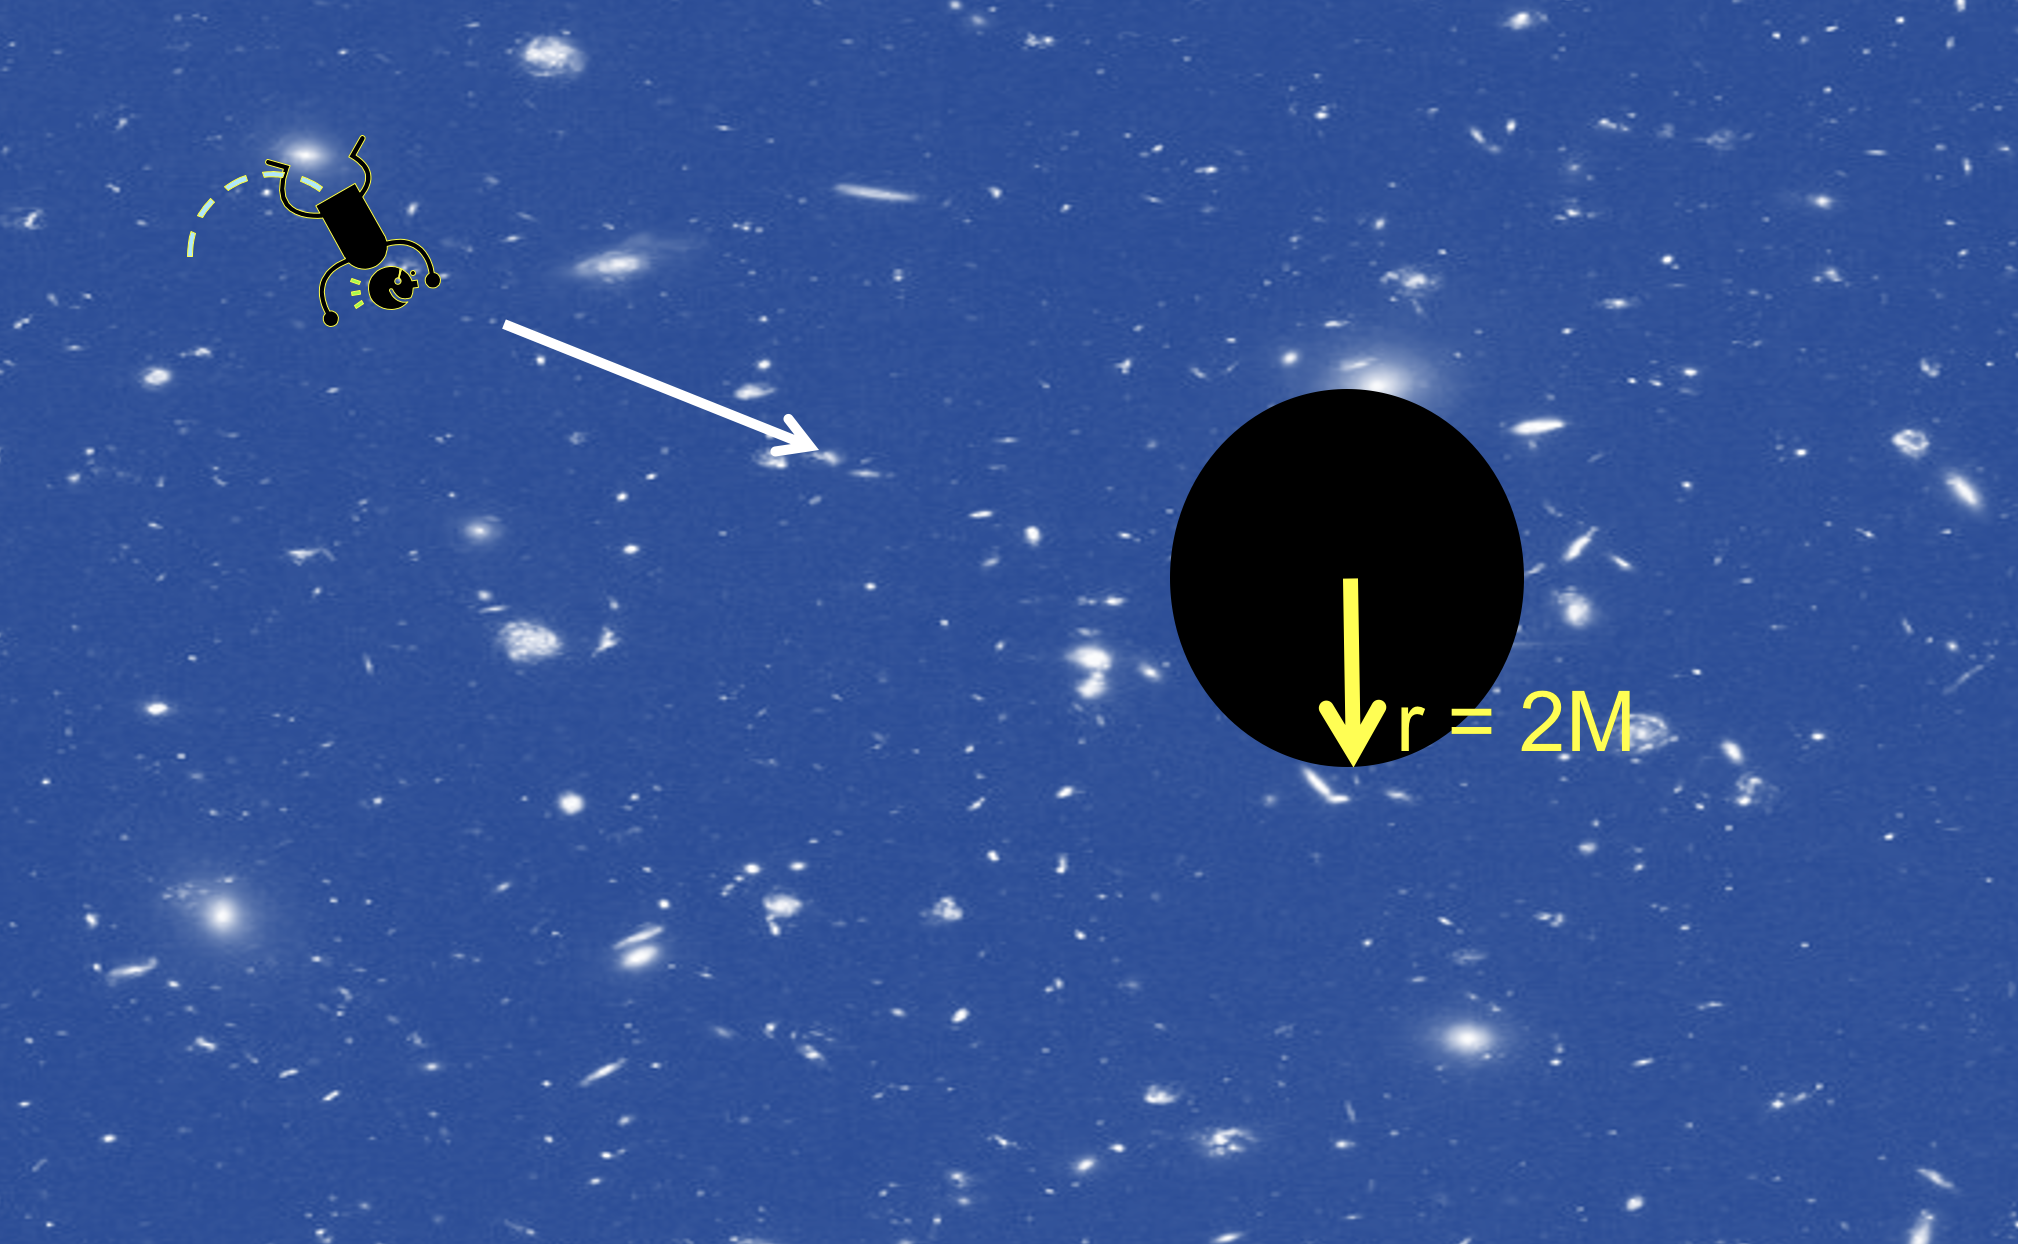
\includegraphics[scale=0.25]{media/shell7.png}}
\textcolor{yellow}{
Vi er tilbake til den {\bf fritt fallende observatøren}. Hun begynner å falle {\bf radialt innover} mot det sorte hullet fra en veldig stor avstand $r\rightarrow\infty$ og med null hastighet $v=0$. Etterhvert vil gravitasjonen fra det sorte hullet akselerere henne innover mot hullet. La oss prøve å finne et uttrykk for hastigheten hennes som funksjon av tida. {\bf Aller først:} Hva er totalenergien $E$ som hun starter med?\\
 \hyperlink{feil_ff1a}{\choicebutton{$E=0$}}\hyperlink{feil_ff1a}{\choicebutton{$E=1$}}\hyperlink{riktig_ff1b}{\choicebutton{$E=m$}}\hyperlink{feil_ff1a}{\choicebutton{$E=m\gamma$}}\hyperlink{feil_ff1a}{\choicebutton{$E=mM$}}
}
}{SIDE 32/41/63}

\colchoiceframe{feil_ff1a}{denim_ff1}{0}{black}{\Huge
\textcolor{yellow}{
Det ble galt. Gå et par sider tilbake og se på uttrykket for energi i tyngdefeltet. Hva blir dette når $r$ er veldig stor og hastigheten er 0?
}
}{SIDE 33/41/63}

\colfullframe{riktig_ff1b}{denim_ff1}{ff2}{-1}{yellow}{\Huge
Det ble riktig. Vi begynner med energi $E=m$ i grensen $r\rightarrow\infty$ og $v=0$.
}{SIDE 34/41/63}

\fullframetwo{ff2}{riktig_ff1b}{ff3}{0}{\footnotesize
For å komme frem til en hastighet $v$ for det fallende legemet/observatøren skal vi følge oppgave 2C.4. Merk at vi først prøver å finne hastigheten $v=dr/dt$ til det fallende legemet målt av langt-vekkobservatøren. Deretter konverterer vi dette uttrykket til hastighet $v_\mathrm{sh}$ målt av en lokal skallobservatør. På den måten kan vi sammenlikne den hastigheten til legemet som funksjon av tiden sett av de to forskjellige observatørene. {\bf Det er sterkt anbefalt at du prøver deg på denne oppgaven. Sett deg en kort tidsgrense i tilfelle du blir stående fast og bruk videoen på neste side til å hjelpe deg kun til de delene der du sitter fast. Dette er en meget god eksempeloppgave for å lære å regne med uttrykket for energi.} (MERK at det i den første oppgaven står ``information above'', det tilsvarer det som står på de 3 foregående sidene!)
}
{
\centerline{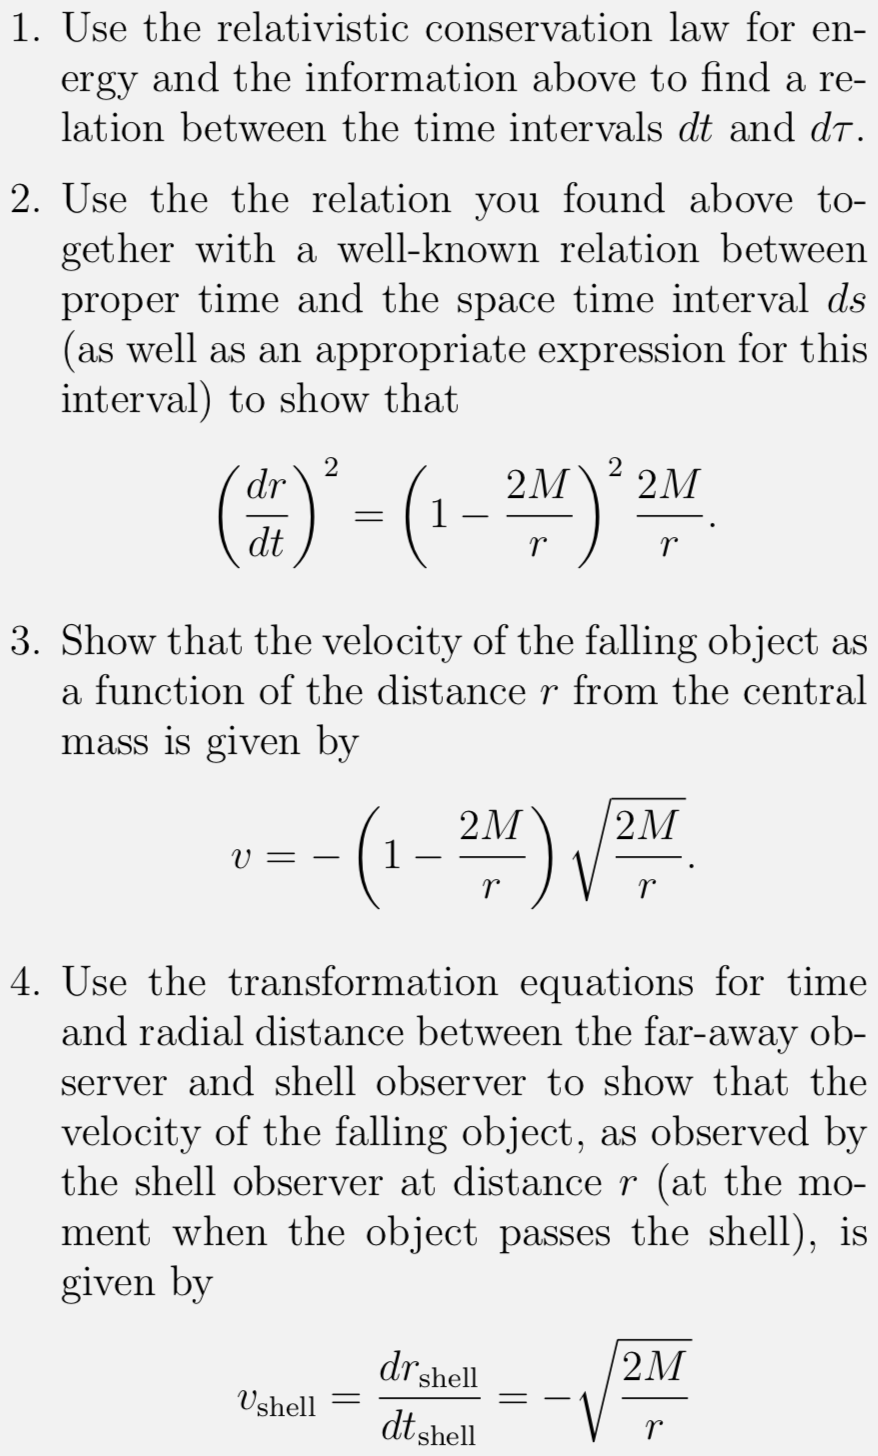
\includegraphics[scale=0.32]{media/2c4.png}}
}{SIDE 35/41/63}

\fullframetwo{ff3}{ff2}{ff4}{0}{\large
Fikk du det til? {\bf I \href{https://www.uio.no/studier/emner/matnat/astro/AST2000/h20/undervisningsmateriell/interaktive-forelesningsnotater/2c/videoer/video2c_11.mp4}{denne videoen} får du hjelp til utledningene.} Når du har forstått hvordan vi kommer frem til uttrykkene skal vi begynne å tolke dem. {\bf La oss begynne} med hastigheten $v$ målt av langt-vekkobservatøren. Kan du forenkle dette uttrykket for store avstander $r$? Kan du finne et annet forenklet uttrykk for disse uttrykkene når $r\rightarrow 2M$?
}
{
\centerline{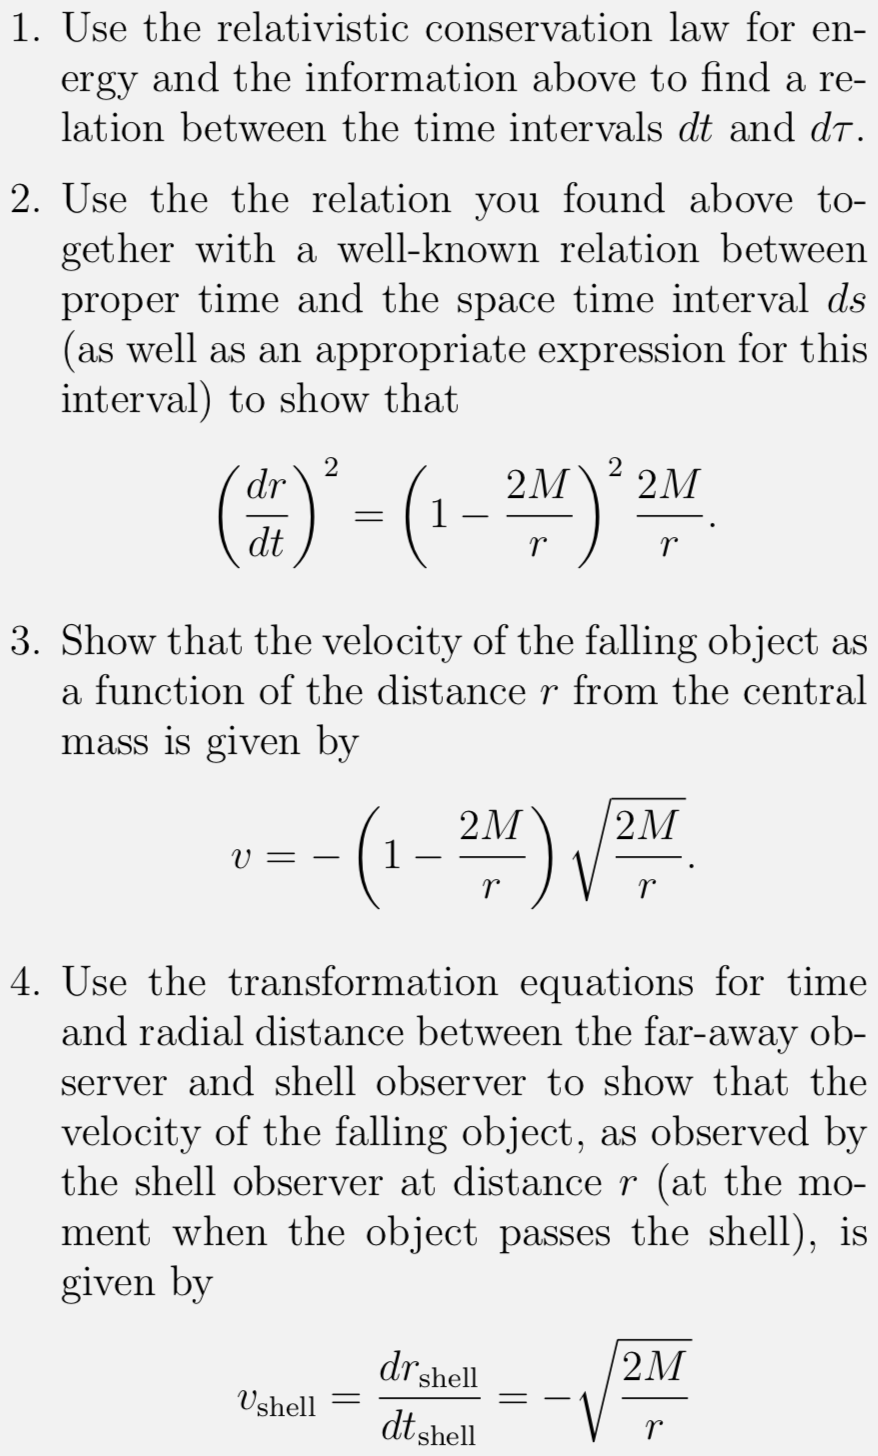
\includegraphics[scale=0.32]{media/2c4.png}}
}{SIDE 36/41/63}

\fullframetwo{ff4}{ff3}{ff5}{0}{\large
Kan du forklare hvorfor
\[
v\approx-\sqrt{\frac{2M}{r}}
\]
når avstanden $r$ er veldig stor, dvs. vi er langt vekk fra tyngdefeltet?
Ser du at dette er likt uttrykket som skallobservatøren måler, hvorfor {\bf må} det være slik?
Og kan du forklare hvorfor
\[
v\approx-\left(1-\frac{2M}{r}\right)
\]
når $r$ er nær (men utenfor) $2M$?
}
{
\centerline{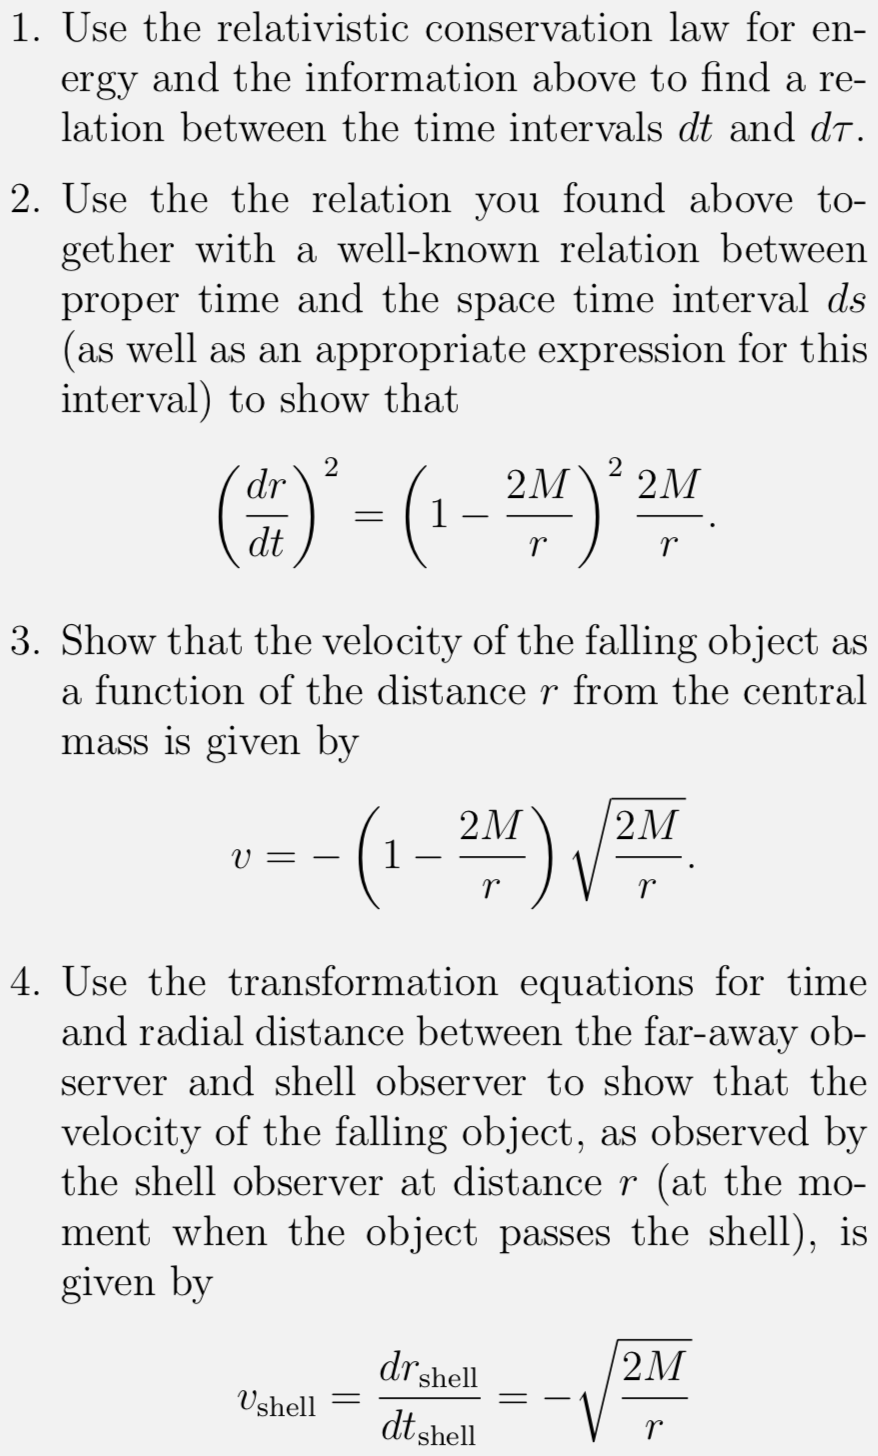
\includegraphics[scale=0.32]{media/2c4.png}}
}{SIDE 37/41/63}


\fullframetwo{ff5}{ff4}{ff6}{0}{\large
\textcolor{red}{Du kan få bruk for formlene under for å svare på disse spørsmålene:}
\begin{itemize}
\item Hva skjer med hastigheten når legemet enda er langt ute men faller innover? Øker eller minker hastigheten?
\item Og hva skjer når legemet nærmer seg hendelsehorisonten, øker eller minker hastigheten ettersom det faller innover?
\item Hvilken hastighet får det rett på hendelsehorisonten?
\end{itemize}
{\bf Minner igjen om at dette er hastighet $v=dr/dt$ målt av langt-vekkobservatøren!}
}
{\large
{\bf Formler du trenger:}
\begin{itemize}
\item \[
v\approx-\sqrt{\frac{2M}{r}}
\]
når avstanden $r$ er veldig stor og
\item \[
v\approx-\left(1-\frac{2M}{r}\right)
\]
når $r$ er nær (men utenfor) $2M$.
\end{itemize}
}{SIDE 38/41/63}

\fullframe{ff6}{ff5}{ff7}{0}{\large
La oss nå se på hastigheten $v_\mathrm{sh}$ {\bf målt av skallobservatøren på det skallet $r$ der ballen passerer på et gitt øyeblikk.:}
\[
v_\mathrm{sh}=-\sqrt{\frac{2M}{r}}
\]
Dette uttrykket gjelder for hele fallet fra start til slutt. Hvilken hastighet vil skallobservatører på skall veldig nær hendelsehorisonten måle at legemet har i det det farer forbi?\\
I \href{https://www.uio.no/studier/emner/matnat/astro/AST2000/h20/undervisningsmateriell/interaktive-forelesningsnotater/2c/videoer/video2c_12.mp4}{denne videoen} får du svar på spørsmålene fra de foregående sidene...
}{SIDE 39/41/63}

\fullframe{ff7}{ff6}{ff7b}{0}{\Huge
Vi avslutter vår studie av det fritt fallende legemet for denne gang ved å se på hva som skjer på innsiden av hendelsehorisonten. \href{https://www.uio.no/studier/emner/matnat/astro/AST2000/h20/undervisningsmateriell/interaktive-forelesningsnotater/2c/videoer/video2c_13.mp4}{Denne videoen} tar for seg litt av hva som skjer der.
}{SIDE 40/41/63}

\fullframe{ff7b}{ff7}{blue_nytema3}{0}{
Oppsummert har vi at:
\begin{itemize}
\item Langt-vekkobservatøren vill aldri se at legemet faller innenfor eventhorisonten. Han vil se at det sakte min sikkert stopper opp på eventhorisonten (vi skal se senere at lyset også blir kraftig rødforskøvet, så han vil til slutt ikke lenger se legemet).
\item Skallobservatører nærmere og nærmere eventhorisonten vil se stadig økende fart på legemet og den vil for skallobservatørene nærmest eventhorisonten nærme seg lysfarta.
\item Den fritt fallende observatøren selv merker ingenting når hun nå går gjennom eventhorisonten, det skjer ikke noe spesielt der for den som faller inn (bortsett fra at gravitasjon etterhvert blir veldig sterkt men det har ikke noe å gjøre med selve hendelsehorisonten, denne effekten kan begynne lenge før $r=2M$). Og i forhold til seg selv har hun alltid hastighet 0.
\end{itemize}
Som vi ser, {\bf tre helt forskjellige hendelseforløp} for 3 forskjellige observatører!
}{SIDE 41/41/63}

\renewcommand{\headline}{GPS}
{
\setbeamercolor{background canvas}{bg=blue}
\begin{frame}
\label{blue_nytema3}
\hyperlink{ff7b}{\pagebutton{\small Forrige side}}
\nytemaside{0}
\textcolor{yellow}{\Large  {\bf MERK: Normalt kommer jeg frem hit etter en dobbelttime fysisk forelesning. Anbefaler sterkt å vente med resten til imorgen!}} Skulle du derimot være frisk og opplagt er det ingenting i veien for å fortsette {\bf etter en skikkelig pause}.
\hyperlink{gps1}{\pagebutton{Hva har relativitetsteorien å gjøre med posisjonsmålinger?}}
\end{frame}
}

\fullframe{gps1}{ff7b}{gps2}{0}{\label{gps}
\centerline{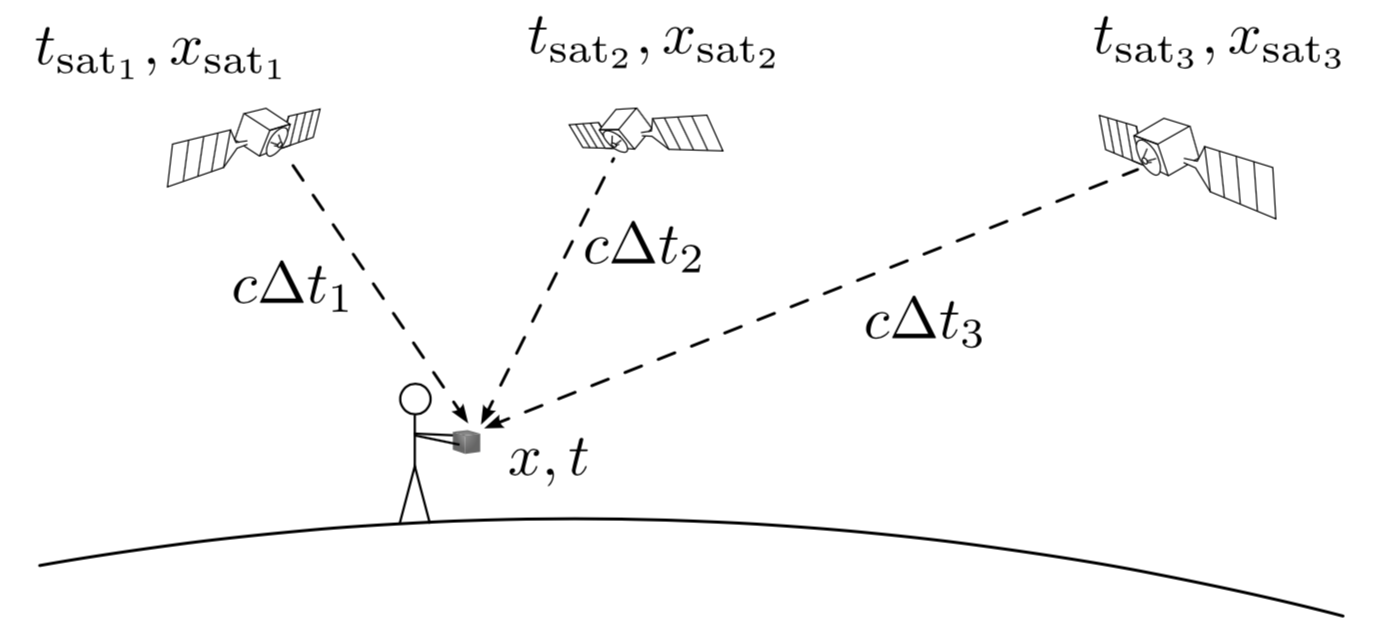
\includegraphics[scale=0.32]{media/gps.png}}
GPS-systemet består av 24 satelitter som går i bane rundt jorden i en høyde av omkring 20\,000km og med omløpstid på 12 timer. Satelittenes posisjon er beregnet veldig nøyaktig til ethvert tidspunkt. Satelittene har klokke ombord og sender kontinuerlig ut signaler med beskjed om nøyaktig fra hvilken posisjon $\vec{x}_{\mathrm{sat},i}$ og i hvilket tidspunkt $t_{\mathrm{sat},i}$ dette signalet ble sendt ut fra satelitt i. Mobilen eller GPS-mottageren din tar imot disse signalene fra 3 (egentlig 4 men det er en annen historie) av disse satelittene. GPS-mottakeren din har også en klokke. Tiden $t$ på mobilen kombinert med posisjonene $\vec{x}_{\mathrm{sat},1}$, $\vec{x}_{\mathrm{sat},2}$, $\vec{x}_{\mathrm{sat},3}$, og tidene $t_{\mathrm{sat},1}$, $t_{\mathrm{sat},2}$ $t_{\mathrm{sat},3}$  som den mottar fra 3 satelitter er nok til å beregne din posisjon $\vec{x}$.
}{SIDE 42/63/63}


\fullframe{gps2}{gps1}{red_gps3}{0}{\Large
\centerline{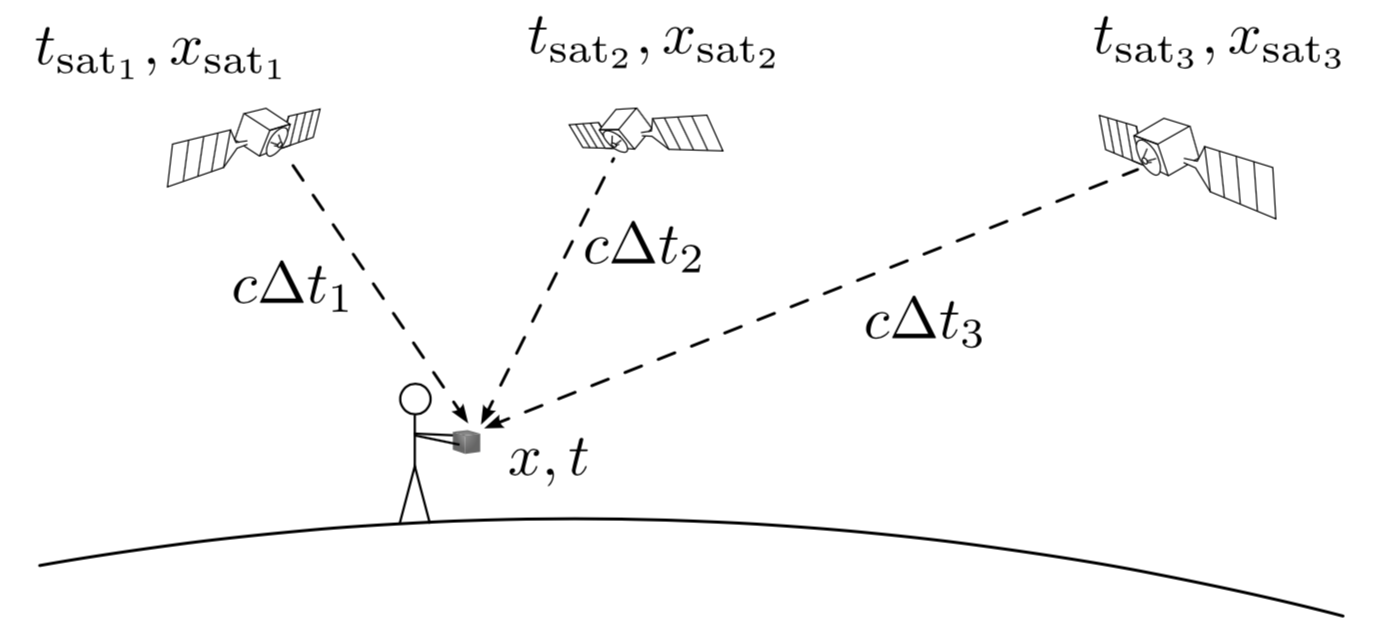
\includegraphics[scale=0.32]{media/gps.png}}
Her har du 3 ukjente som er de 3 komponentene av posisjonsvektoren din $\vec{x}$. Kan du skrive opp 3 likninger for å løse disse? Dvs. de 3 likningene som GPS-mottakeren løser for å finne din posisjon? {\bf Merk at du ikke skal løse likningene, kun skrive de opp!}. Bruk gjerne SI-enheter nå isteden for relativistiske enheter.
}{SIDE 43/63/63}

\colfullframenotxt{red_gps3}{gps2}{gps4}{0}{red}{\Large
\centerline{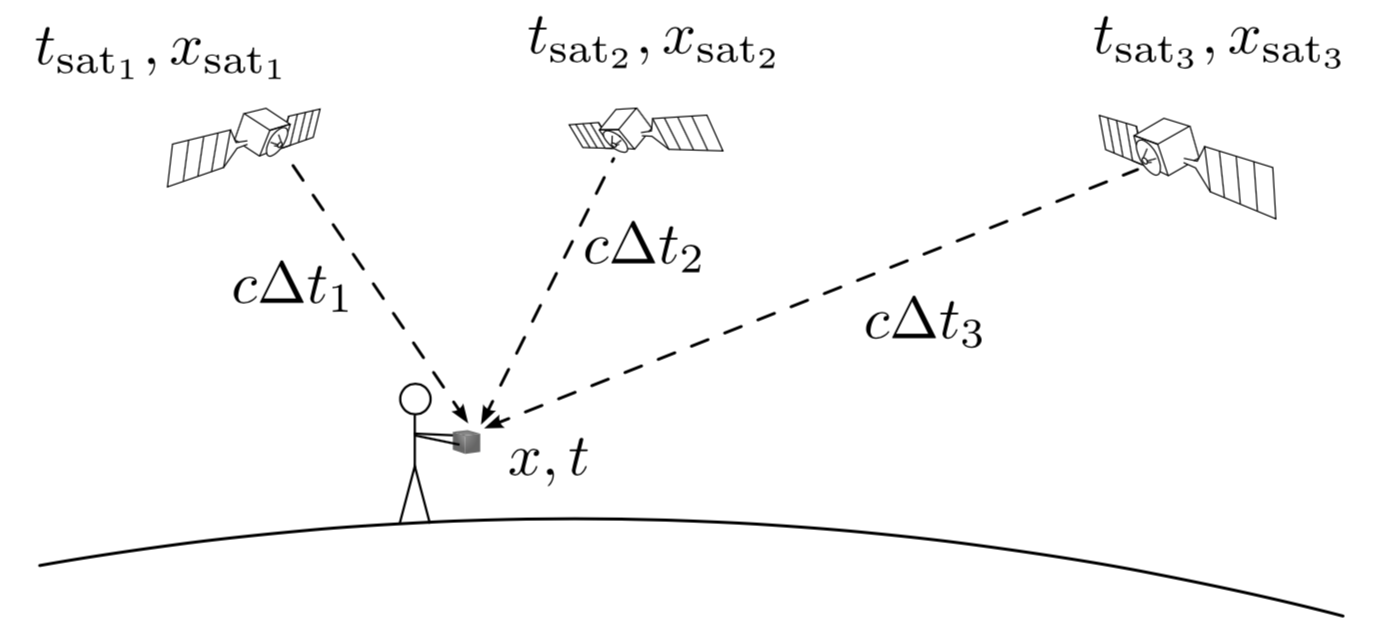
\includegraphics[scale=0.32]{media/gps.png}}
\textcolor{yellow}{
{\Large Fikk du det til???} Trenger du et hint?}
\hyperlink{gps4}{\pagebutton{Neida, fikk det til jeg!}}\hyperlink{red_gps3_b}{\pagebutton{Gjerne et hint ja!}}
\textcolor{red}{Strekning er lik fart ganger tid. Hvor lang tid bruker hver av signalene fra satelitten frem til GPS-mottakeren? Det er 3 slike signaler!}
}{SIDE 44/63/63}

\colfullframetxt{red_gps3_b}{gps2}{gps4}{0}{red}{Nå har jeg det!}{\Large
\centerline{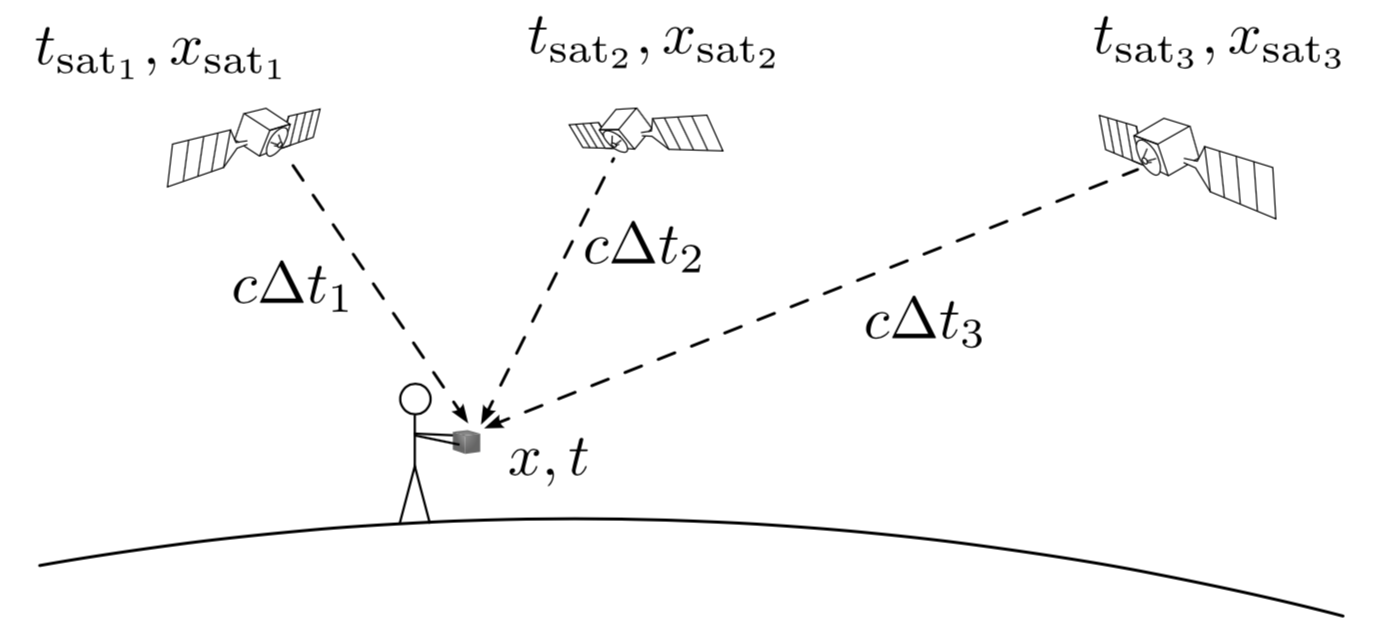
\includegraphics[scale=0.32]{media/gps.png}}
\textcolor{yellow}{
{\Large Fikk du det til???} Trenger du et hint?}
{\pagebutton{Neida, fikk det til jeg!}}{\pagebutton{Gjerne et hint ja!}}
\textcolor{yellow}{Strekning er lik fart ganger tid. Hvor lang tid bruker hver av signalene fra satelitten frem til GPS-mottakeren? Det er 3 slike signaler!}
}{SIDE 44/63/63}



\fullframe{gps4}{red_gps3}{gps5}{1}{\Large
\centerline{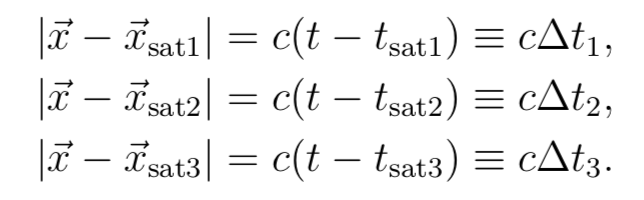
\includegraphics[scale=0.7]{media/gps2.png}}
Fikk du disse likningene? Her er $\Delta t_i$ tiden det tar for hver av de 3 signalene å gå fra satelitt og frem til mottaker. Vi skal ikke løse disse likningene i sin helhet her, men jeg vi prøve å overbevise deg om at svaret, f.eks. for x-komponenten kommer til å inneholde flere ledd av typen
\[
x=\mathrm{et\ eller\ annet\ ganger\ }c\Delta t_1 + ...
\]
høres det sannsynlig ut?
}{SIDE 45/63/63}

\fullframe{gps5}{gps4}{gps6}{0}{\Large
Hvis du er enig i det, så la oss som eksempel bare anta for enkelhetsskyld til første orden at
\[
x\approx c\Delta t_1
\]
(løsningen kommer til å ha mange ledd av denne typen til første orden)
Her er jo $\Delta t_1$ tiden det tar fra signalet ble sendt ut fra satelitt 1 til det blir mottatt på GPS-mottakeren, altså
\[
\Delta t_1=t-t_{\mathrm{sat},1}
\]
{\bf Hvis tidsintervallet $\Delta t_1$ blir målt feil med kun 1 mikrosekund ($10^{-6}$ sekunder}, hvor stor blir feilen i posisjon??
\hyperlink{feil_gps5a}{\choicebutton{$\Delta x\approx 3$ meter}}\hyperlink{feil_gps5a}{\choicebutton{$\Delta x\approx 30$ meter}}\\
\hyperlink{riktig_gps5b}{\choicebutton{$\Delta x\approx 300$ meter}}\hyperlink{feil_gps5a}{\choicebutton{$\Delta x\approx 3$ kilometer}}
}{SIDE 46/63/63}


\colchoiceframe{feil_gps5a}{gps5}{0}{black}{\Huge
\textcolor{yellow}{
Her var du litt rask, prøv igjen, dette får du til!
}
}{SIDE 47/63/63}

\colfullframetxt{riktig_gps5b}{gps5}{gps6}{-1}{yellow}{mener du et relativistisk problem? Ja, saktens...}{\Huge
Nettopp! {\bf Hele 300 meter feil med bare et mikrosekund bom på tiden.} Da må tidsmålingen være {\bf veldig} nøyaktig for at du skal få meningsfull posisjon med GPS. Men ser du et problem her???
}{SIDE 48/63/63}


\fullframetxt{gps6}{riktig_gps5b}{gps7}{0}{Tror jeg husker...}{\Large
Vi jordboere og satelittene er vel begge {\bf skallobservatører} i hvert sitt skall? Vi går rundt med omkring fast avstand $r$ til jordas sentrum, samme gjør satelittene men med en annen $r$. {\bf Dermed går satelittklokkene med en annen hastighet enn våre klokker!}. Hvordan var nå dette igjen, går satelittklokkene {\bf fortere} eller {\bf saktere} enn våre klokker?
}{SIDE 49/63/63}

\fullframenotxt{gps7}{gps6}{gps8}{0}{\small
Var det ikke slik at tiden går saktere {\bf nede i et tyngdefelt}? Altså at tiden vår går saktere enn klokkene i satelitten? Vi hadde:
\[
\Delta t_\mathrm{sh}=\sqrt{\sst}\Delta t
\]
{\bf Men hvor mye saktere går klokkene våre? Blir det størrelseorden mikrosekund?} Isåfall kan det ha stor effekt på posisjonsmålinger med GPS. Men det er en ting til: Satelittene har en ganske høy hastighet i forhold til oss, da kommer også spesiell relativitetsteori inn! Men hvilken vei virker den? Går klokkene våre fortere eller saktere enn satelittens klokker på grunn av spesiell relativitet?\hyperlink{gps7_b}{\pagebutton{Jeg har tenkt og vet svaret!}}\textcolor{white}{
Var det ikke slik at $\Delta t=\gamma\Delta\tau$? Der $t$ er lab-tida, altså tida vår mens $\tau$ er egentida til satelitten (toget)? Husk at $\gamma$ er en forstørrelsefaktor. Vi husker at vi ser alt i saktefilm i toget slik at tiden mellom to tikk på klokka i toget tok {\bf lenger tid} på våre klokker, $\Delta t>\Delta\tau$. Altså at våre klokker går {\bf raskere} enn satelittklokkene!. \textcolor{white}{Denne er nøyaktig motsatt av den generell-relativistiske effekten der våre klokker går fortere enn satelittklokkene på grunn av tyngdefeltet. {\bf De to effektene motvirker altså hverandre, men nuller de hverandre ut??} Det må vi sjekke nå!}}
}{SIDE 50/63/63}

\fullframe{gps7_b}{gps6}{gps8}{0}{\small
Var det ikke slik at tiden går saktere {\bf nede i et tyngdefelt}? Altså at tiden vår går saktere enn klokkene i satelitten? Vi hadde:
\[
\Delta t_\mathrm{sh}=\sqrt{\sst}\Delta t
\]
{\bf Men hvor mye saktere går klokkene våre? Blir det størrelseorden mikrosekund?} Isåfall kan det ha stor effekt på posisjonsmålinger med GPS. Men det er en ting til: Satelittene har en ganske høy hastighet i forhold til oss, da kommer også spesiell relativitetsteori inn! Men hvilken vei virker den? Går klokkene våre fortere eller saktere enn satelittens klokker på grunn av spesiell relativitet?{\pagebutton{Jeg har tenkt og vet svaret!}}
Var det ikke slik at $\Delta t=\gamma\Delta\tau$? Der $t$ er lab-tida, altså tida vår mens $\tau$ er egentida til satelitten (toget)? Husk at $\gamma$ er en forstørrelsefaktor. Vi husker at vi ser alt i saktefilm i toget slik at tiden mellom to tikk på klokka i toget tok {\bf lenger tid} på våre klokker, $\Delta t>\Delta\tau$. Altså at våre klokker går {\bf raskere} enn satelittklokkene!. \textcolor{red}{Denne er nøyaktig motsatt av den generell-relativistiske effekten der våre klokker går saktere enn satelittklokkene på grunn av tyngdefeltet. {\bf De to effektene motvirker altså hverandre, men nuller de hverandre ut??} Det må vi sjekke nå!}
}{SIDE 50/63/63}

\fullframe{gps8}{gps7}{gps9}{1}{\large
Vi skal se at \ss-geometrien inneholder både generell og spesiell relativitetsteori sammen slik at også effektene av hastighet er med. For å finne hvor mye fortere eller saktere våre klokker går i forhold til satelittklokkene, trenger vi å finne forskjellen mellom et tidsintervall $\Delta\tau_\mathrm{sat}$ på en satelittklokke, f.eks. to tikk på satelittklokken, og hvor lang tid $\Delta\tau_\mathrm{jord}$ det går på våre klokker mellom disse to tikkene. Er denne forskjellen så stor at den kan medføre at vi beregner gale reisetider til signalene og dermed gale posisjoner med GPS? {\bf Merk} at vi her skal bruke {\bf egentid $\Delta\tau$} for både satelittene og oss selv. Altså tid målt på klokker som står fast på satelittene og andre som står fast på oss. {\bf Men begge disse egentidene tikker med forskjellig hastighet.}
}{SIDE 51/63/63}

\fullframe{gps9}{gps8}{red_gps10}{0}{\large
Har du lagt merke til at vi egentlig skal transformere tidsintervall mellom {\bf to skallobservatører?} Gitt at det tar et tidsintervall $\Delta\tau_\mathrm{sat}$ mellom to tikk på klokka til satelitten, så vil vi finne hvor lang tid  $\Delta\tau_\mathrm{jord}$ det tar på vår klokke mellom de to tikkene. Vi har oss selv som er skallobservatørene på jorda med fast avstands-koordinat $r_\mathrm{jord}$ og med en tangensialhastighet (på grunn av jordas rotasjon) på $v_{\phi,\mathrm{jord}}$ langs skallet vårt. Satelittene er også skallobservatører som er fast på skallet i avstand $r_\mathrm{sat}$ og med en tangensialhastighet langs skallet sitt som er $v_{\phi,\mathrm{sat}}$ gitt av banehastigheten.{\bf Men vi har så langt bare utledet transformasjonen av et tidsintervall $\Delta t$ for langt-vekkobservatøren til et skalltidsintervall $\Delta t_\mathrm{sh}$ for et gitt skall! Vi har ikke utledet denne transformasjonen mellom to skall som er det vi trenger her!}. \textcolor{red}{Men vi har egentlig det vi trenger for å gjøre denne transformasjonen, ser du det??}
}{SIDE 52/63/63}

\colfullframenotxt{red_gps10}{gps9}{gps11}{0}{red}{\Huge
\textcolor{yellow}{
Her bør du prøve å se om du finner en løsning. Dette kan være en typisk oppgave...\hyperlink{red_gps10_b}{\pagebutton{Hint? Please?}}}\textcolor{red}{
Det fikk du på forrige side, selv om det ikke står eksplisitt at det er et hint...}
}{SIDE 53/63/63}

\colfullframetxt{red_gps10_b}{gps9}{gps11}{0}{red}{Jeg har tenkt og tenkt...}{\Huge
\textcolor{yellow}{
Her bør du prøve å se om du finner en løsning. Dette kan være en typisk oppgave...{\pagebutton{Hint? Please?}}
Det fikk du på forrige side, selv om det ikke står eksplisitt at det er et hint...
}
}{SIDE 53/63/63}


\fullframetxt{gps11}{red_gps10}{gps12}{1}{Absolutt, dette kan jeg!}{
Prinsippet er som følger:
\begin{itemize}
\item La oss ta f.eks. to tikk på (egentids-)klokka til satelitten. Vi kaller tidsintervallet mellom disse for $\Delta\tau_\mathrm{sat}$.
\item Vi vet dermed at vi kan regne dette om til et tidsintervall $\Delta t$ for langt-vekkobservatøren. For langt-vekkobservatøren tar det altså et tidsintervall $\Delta t$ mellom de to tikkene på satelittklokka.
\item Men vi kan igjen regne om et tidsintervall for langt-vekkobservatøren til et tidsintervall på {\bf vårt skall}. Altså vi kan finne ut hvor lang tid det tar på våre (egentids-)klokker $\Delta\tau_\mathrm{jord}$ for et tidsintervall $\Delta t$ på langt-vekk-klokka.
\item Men siden tidsintervallet $\Delta t$ på langt-vekk-klokka tilsvarer tidsintervallet $\Delta\tau_\mathrm{sat}$ mellom to tikk på satelittklokka, så har vi altså funnet tidsintervallet $\Delta\tau_\mathrm{jord}$ målt av oss mellom de to tikkene på satelittklokka
\end{itemize}
Vi trenger altså å finne noen uttrykk for $\Delta\tau_\mathrm{sat}$ og $\Delta\tau_\mathrm{jord}$, begge uttrykt ved det felles langt-vekk-tidsintervallet $\Delta t$. {\bf Kan du se hvordan vi kan finne et slikt uttrykk?}
}{SIDE 54/63/63}


\fullframenotxt{gps12}{gps11}{gps13}{0}{
La oss begynne med $\Delta\tau_\mathrm{sat}$, kan du finne et uttrykk for denne som også inneholder $\Delta t$?\hyperlink{gps12_b}{\pagebutton{Hint?}}\textcolor{white}{
Et egettidsintervall mellom to eventer er vel lik tidromsintervallet mellom disse eventene? Og hvordan ser tidromsintervallet ut?{Ahaa.....}
Siden vi nå skal gå fra et skall til et annet så kan vi ikke anta lokalt inertialsystem, da må vi bruke full \ss-geometri:
\[
\Delta\tau_\mathrm{sat}^2=\Delta s^2=\sst\Delta t^2-\frac{\Delta r_\mathrm{sat}^2}{\sst}-r_\mathrm{sat}^2\Delta\phi_\mathrm{sat}^2
\]
der $\Delta s$ og $\Delta t$ altså er tidroms- og langt-vekktidsintervall mellom de to tikkene på satelittklokka.{OK!}
{\bf Men satelitten endrer vel ikke $r$-poisjon?} Den er jo fast på et skall, så vi får vel $\Delta r_\mathrm{sat}=0$ som gir
\[
\Delta\tau_\mathrm{sat}^2=\sst\Delta t^2-r_\mathrm{sat}^2\Delta\phi_\mathrm{sat}^2
\]}
}{SIDE 55/63/63}

\fullframenotxt{gps12_b}{gps11}{gps13}{0}{
La oss begynne med $\Delta\tau_\mathrm{sat}$, kan du finne et uttrykk for denne som også inneholder $\Delta t$?{\pagebutton{Hint?}}
Et egettidsintervall mellom to eventer er vel lik tidromsintervallet mellom disse eventene? Og hvordan ser tidromsintervallet ut?\hyperlink{gps12_c}{\pagebutton{Ahaa.....}}\textcolor{white}{
Siden vi nå skal gå fra et skall til et annet så kan vi ikke anta lokalt inertialsystem, da må vi bruke full \ss-geometri:
\[
\Delta\tau_\mathrm{sat}^2=\Delta s^2=\sst\Delta t^2-\frac{\Delta r_\mathrm{sat}^2}{\sst}-r_\mathrm{sat}^2\Delta\phi_\mathrm{sat}^2
\]
der $\Delta s$ og $\Delta t$ altså er tidroms- og langt-vekktidsintervall mellom de to tikkene på satelittklokka.{OK!}
{\bf Men satelitten endrer vel ikke $r$-poisjon?} Den er jo fast på et skall, så vi får vel $\Delta r_\mathrm{sat}=0$ som gir
\[
\Delta\tau_\mathrm{sat}^2=\sst\Delta t^2-r_\mathrm{sat}^2\Delta\phi_\mathrm{sat}^2
\]}
}{SIDE 55/63/63}

\fullframenotxt{gps12_c}{gps11}{gps13}{0}{
La oss begynne med $\Delta\tau_\mathrm{sat}$, kan du finne et uttrykk for denne som også inneholder $\Delta t$?{\pagebutton{Hint?}}
Et egettidsintervall mellom to eventer er vel lik tidromsintervallet mellom disse eventene? Og hvordan ser tidromsintervallet ut?{\pagebutton{Ahaa.....}}
Siden vi nå skal gå fra et skall til et annet så kan vi ikke anta lokalt inertialsystem, da må vi bruke full \ss-geometri:
\[
\Delta\tau_\mathrm{sat}^2=\Delta s^2=\sst\Delta t^2-\frac{\Delta r_\mathrm{sat}^2}{\sst}-r_\mathrm{sat}^2\Delta\phi_\mathrm{sat}^2
\]
der $\Delta s$ og $\Delta t$ altså er tidroms- og langt-vekktidsintervall mellom de to tikkene på satelittklokka.\hyperlink{gps12_d}{\pagebutton{OK!}}\textcolor{white}{
{\bf Men satelitten endrer vel ikke $r$-poisjon?} Den er jo fast på et skall, så vi får vel $\Delta r_\mathrm{sat}=0$ som gir
\[
\Delta\tau_\mathrm{sat}^2=\sst\Delta t^2-r_\mathrm{sat}^2\Delta\phi_\mathrm{sat}^2
\]}
}{SIDE 55/63/63}


\fullframe{gps12_d}{gps11}{gps13}{0}{
La oss begynne med $\Delta\tau_\mathrm{sat}$, kan du finne et uttrykk for denne som også inneholder $\Delta t$?{\pagebutton{Hint?}}
Et egettidsintervall mellom to eventer er vel lik tidromsintervallet mellom disse eventene? Og hvordan ser tidromsintervallet ut?{\pagebutton{Ahaa.....}}
Siden vi nå skal gå fra et skall til et annet så kan vi ikke anta lokalt inertialsystem, da må vi bruke full \ss-geometri:
\[
\Delta\tau_\mathrm{sat}^2=\Delta s^2=\sst\Delta t^2-\frac{\Delta r_\mathrm{sat}^2}{\sst}-r_\mathrm{sat}^2\Delta\phi_\mathrm{sat}^2
\]
der $\Delta s$ og $\Delta t$ altså er tidroms- og langt-vekktidsintervall mellom de to tikkene på satelittklokka.{\pagebutton{OK!}}
{\bf Men satelitten endrer vel ikke $r$-poisjon?} Den er jo fast på et skall, så vi får vel $\Delta r_\mathrm{sat}=0$ som gir
\[
\Delta\tau_\mathrm{sat}^2=\sst\Delta t^2-r_\mathrm{sat}^2\Delta\phi_\mathrm{sat}^2
\]
}{SIDE 55/63/63}

\fullframenotxt{gps13}{gps12}{gps14}{1}{
Vi hadde altså
\[
\Delta\tau_\mathrm{sat}^2=\left(1-\frac{2M}{r_\mathrm{sat}}\right)\Delta t^2-r_\mathrm{sat}^2\Delta\phi_\mathrm{sat}^2
\]
Men vi har en $\Delta\phi_\mathrm{sat}$ her! Hadde det ikke vært bedre å få inn satelitthastigheten $v_{\phi,\mathrm{sat}}$? Hvordan kan du gjøre det?\hyperlink{gps13_b}{\pagebutton{Jeg har tenkt og har et forslag...}}\textcolor{white}{
Vi vet jo fra celestmekanikk at tangensialhastighet er gitt ved $v_\phi=r\dot{\phi}=r\Delta\phi/\Delta t$, ikke sant? Omskrevet har vi da $r\Delta\phi=v_\phi\Delta t$. Insatt gir det oss
\[
\Delta\tau_\mathrm{sat}^2=\Delta t^2\left(1-\frac{2M}{r_\mathrm{sat}}-v_{\phi,\mathrm{sat}}^2\right)
\]}
}{SIDE 56/63/63}

\fullframe{gps13_b}{gps12}{gps14}{1}{
Vi hadde altså
\[
\Delta\tau_\mathrm{sat}^2=\left(1-\frac{2M}{r_\mathrm{sat}}\right)\Delta t^2-r_\mathrm{sat}^2\Delta\phi_\mathrm{sat}^2
\]
Men vi har en $\Delta\phi_\mathrm{sat}$ her! Hadde det ikke vært bedre å få inn satelitthastigheten $v_{\phi,\mathrm{sat}}$? Hvordan kan du gjøre det?{\pagebutton{Jeg har tenkt og har et forslag...}}
Vi vet jo fra celestmekanikk at tangensialhastighet er gitt ved $v_\phi=r\dot{\phi}=r\Delta\phi/\Delta t$, ikke sant? Omskrevet har vi da $r\Delta\phi=v_\phi\Delta t$. Insatt gir det oss
\[
\Delta\tau_\mathrm{sat}^2=\Delta t^2\left(1-\frac{2M}{r_\mathrm{sat}}-v_{\phi,\mathrm{sat}}^2\right)
\]
}{SIDE 56/63/63}

\fullframe{gps14}{gps13}{gps15}{2}{
Vi kan bruke nøyaktig samme tankegang for oss selv som skallobservatører og komme frem til nøyaktig samme uttrykk:
\[
\Delta\tau_\mathrm{jord}^2=\Delta t^2\left(1-\frac{2M}{r_\mathrm{jord}}-v_{\phi,\mathrm{jord}}^2\right)
\]
Sammen med uttrykket for satelitten fra forrige side
\[
\Delta\tau_\mathrm{sat}^2=\Delta t^2\left(1-\frac{2M}{r_\mathrm{sat}}-v_{\phi,\mathrm{sat}}^2\right)
\]
kan vi nå finne forholdet $\Delta\tau_\mathrm{jord}/\Delta\tau_\mathrm{sat}$ som sier oss forholdet mellom et tidsintervall på satelittklokke og vår egen klokke. Vi deler rett og slett de to likningen på hverandre og tar kvadratroten:
\[
\frac{\Delta\tau_\mathrm{jord}}{\Delta\tau_\mathrm{sat}}=\sqrt{\frac{1-\frac{2M}{r_\mathrm{jord}}-v_{\phi,\mathrm{jord}}^2}{1-\frac{2M}{r_\mathrm{sat}}-v_{\phi,\mathrm{sat}}^2}}
\]
Legg merke til at tidsintervallet $\Delta t$ blir forkortet vekk siden vi ser på det samme tidsintervallet (for langt-vekkobservatøren) i begge tilfeller.
}{SIDE 57/63/63}

\fullframe{gps15}{gps14}{gps16}{0}{{\Huge
{\bf Pent lite uttrykk, hva?}
\[
\frac{\Delta\tau_\mathrm{jord}}{\Delta\tau_\mathrm{sat}}=\sqrt{\frac{1-\frac{2M}{r_\mathrm{jord}}-v_{\phi,\mathrm{jord}}^2}{1-\frac{2M}{r_\mathrm{sat}}-v_{\phi,\mathrm{sat}}^2}}
\]}
Hvis vi lar tyngdefeltet her bli veldig svakt, si $M\rightarrow0$ og vi lar oss selv stå i ro $v_{\phi,\mathrm{jord}}=0$, ser du hva vi får da? Står det ikke da egentlig her at $\Delta t=\gamma\Delta\tau$? Slik ser vi at den spesielle relativitetsteorien er innebakt i \ss-geometrien, når tyngdefeltet er lite får vi tilbake Lorentz.
}{SIDE 58/63/63}

\fullframe{gps16}{gps15}{gps17}{0}{
\[
\frac{\Delta\tau_\mathrm{jord}}{\Delta\tau_\mathrm{sat}}=\sqrt{\frac{1-\frac{2M}{r_\mathrm{jord}}-v_{\phi,\mathrm{jord}}^2}{1-\frac{2M}{r_\mathrm{sat}}-v_{\phi,\mathrm{sat}}^2}}
\]
La oss prøve å sette inn tall: Vi kjenner avstanden til jordas overflate $r_\mathrm{jord}\approx6000$\;km og satelittene går i en høyde av 20\,000\,km som betyr  $r_\mathrm{sat}\approx26000$\,km. Det holder med omtrentlige tall her, vi skal jo kun gjøre et overslag for å finne størrelseorden. Et punkt på jordoverflaten snurrer en gang rundt i løpet av omkring 24 timer, altså er $v_{\phi,\mathrm{jord}}=2\pi\times6000/(24\times3600)$\,km/s og satelittene bruker 12 timer på en runde, altså $v_{\phi,\mathrm{sat}}=2\pi\times26000/(12\times3600)$\,km/s. Vi fant på forrige forelesning at jordas masse i meter er $M=4.45$\,mm. {\bf Husk at hastighetene må deles på lyshastigheten for å få relativistiske enheter!}. {\huge Sett inn disse tallene i telleren og nevneren av brøken hver for seg! Hvilke tall fikk du?}\textcolor{red}{Det er {\bf svært viktig} at du faktisk gjør dette, du kommer til å oppdage noe!}
}{SIDE 59/63/63}


\fullframe{gps17}{gps16}{gps18}{0}{\huge
Fikk du noe alla $0.99999999$ og kanskje til slutt noen andre siffer? For både telleren og nevneren? Fikk du ikke det, har du gjort noe galt, du {\bf skal få det!}.\textcolor{red}{Men dele to slike tall på hverandre? Og deretter ta kvadratroten??? {\bf Her er det duket for store numeriske feil!!!}}
}{SIDE 60/63/63}


\fullframetxt{gps18}{gps17}{gps19}{0}{Jeg tror jeg vet det...}{\large
\[
\frac{\Delta\tau_\mathrm{jord}}{\Delta\tau_\mathrm{sat}}=\sqrt{\frac{1-\frac{2M}{r_\mathrm{jord}}-v_{\phi,\mathrm{jord}}^2}{1-\frac{2M}{r_\mathrm{sat}}-v_{\phi,\mathrm{sat}}^2}}
\]
Dette skjer selvfølgelig fordi både $2M/r$ og $v^2$ er {\bf mye mindre} enn 1 både i teller og nevner. Vi har altså 1 og trekker fra noen bittesmå tall. {\bf Dette vil alltid skje når du bruker relativitetsteori på ``hverdagen'', altså lave hastigheter og svake gravitasjonsfelt.}{\huge Hva gjør vi da??? {\bf Forslag til løsning?}}
}{SIDE 61/63/63}


\fullframenotxt{gps19}{gps18}{gps20}{0}{\large
\[
\frac{\Delta\tau_\mathrm{jord}}{\Delta\tau_\mathrm{sat}}=\sqrt{\frac{1-\frac{2M}{r_\mathrm{jord}}-v_{\phi,\mathrm{jord}}^2}{1-\frac{2M}{r_\mathrm{sat}}-v_{\phi,\mathrm{sat}}^2}}
\]
Jaaaa, altså hvis $2M/r$ og $v^2$ er små størrelser, hvorfor ikke {\bf rekkeutvikle} i disse? Da skulle vi ende opp med polynomer som vi fint kan regne uten numeriske problemer. {\bf Dette pleier å være løsningen!}. Men hvordan vil du gå frem for å rekkeutvikle her?\hyperlink{gps19_b}{\pagebutton{Tjaaaaaa...}}\textcolor{white}{
I {denne videoen får du hjelp...}}
}{SIDE 62/63/63}

\fullframe{gps19_b}{gps18}{gps20}{0}{\large
\[
\frac{\Delta\tau_\mathrm{jord}}{\Delta\tau_\mathrm{sat}}=\sqrt{\frac{1-\frac{2M}{r_\mathrm{jord}}-v_{\phi,\mathrm{jord}}^2}{1-\frac{2M}{r_\mathrm{sat}}-v_{\phi,\mathrm{sat}}^2}}
\]
Jaaaa, altså hvis $2M/r$ og $v^2$ er små størrelser, hvorfor ikke {\bf rekkeutvikle} i disse? Da skulle vi ende opp med polynomer som vi fint kan regne uten numeriske problemer. {\bf Dette pleier å være løsningen!}. Men hvordan vil du gå frem for å rekkeutvikle her?\hyperlink{gps19b}{\pagebutton{Tjaaaaaa...}}
I \href{https://www.uio.no/studier/emner/matnat/astro/AST2000/h20/undervisningsmateriell/interaktive-forelesningsnotater/2c/videoer/video2c_14.mp4}{denne videoen får du hjelp...}
}{SIDE 62/63/63}



\fullframe{gps20}{gps19}{oppsummering}{1}{
Vi får altså:
\[
\frac{\Delta\tau_\mathrm{jord}}{\Delta\tau_\mathrm{sat}}\approx1+\left(\frac{M}{r_\mathrm{sat}}-\frac{M}{r_\mathrm{jord}}\right)+\frac{1}{2}(v_{\phi,\mathrm{sat}}^2-v_{\phi,\mathrm{jord}}^2)
\]
Her har vi altså et uttrykk for hvor mye fortere en klokke går enn den andre. Anta at klokka i GPS-satelittene ble synkronisert med jord-klokker i det øyeblikk satelittene begynte å bli operasjonelle. Et døgn, nøyaktig 24 timer senere, målt på satelittklokkene, hvor mye har klokkene på jorda gått? Hvis vi setter $\Delta\tau_\mathrm{sat}=24$\,timer så ser vi at det første leddet etter 1-tallet, det leddet som korrigere for relativistiske effekter fra tyngdefeltet gir oss -49 mikrosekunder mens det andre leddet som avhenger av hastighet og dermed kommer fra spesiell relativitetsteori gir oss +7 mikrosekunder. Totalt er det da en forskjell mellom GPS-klokker og jordklokker på 42 mikrosekunder! Hvis vi igjen ser på løsningen av likningene for å finne din posisjon så gir dette en posisjonsfeil av størrelseorden $\Delta x=c\times42\mu\mathrm{s}\approx13$\,km!!!. {\bf Etter et døgn ville GPS-systemet vært ubruklig hvis det ikke tar hensyn til relativistiske korreksjoner, både fra generell og spesiell relativitetsteori!}
}{SIDE 63/63/63}

\begin{frame}
\label{oppsummering}
\hyperlink{gps20}{\pagebutton{\small Forrige side}}\href{https://nettskjema.no/a/171674}{\Changey[1][yellow]{2} \Changey[1][yellow]{-2}}
\tiny
{\bf Du er ferdig med forelesning 2 av 2 i del 2C.}. Du bør nå:
\begin{itemize}
\item Du bør kjenne til de 3 observatørene som brukes i et \ss-tidrom. Du bør vite hvordan disse måler avstander og tidsintervaller mellom eventer og hvilke koordianter de bruker.
\item Du bør kjenne til betingelsene for å kunne bruke antakelsen om lokalt inertialsystem og hva det innebærer.
\item Du bør kunne bruke uttrykket for $\Delta s$ i \ss-geometri.
\item Du bør kunne bruke prinsippet om maksimal aldring til å utlede energi og bevegelsemengdebevaring i Lorentz- og i \ss-geometri.
\item Du bør kjenne til og kunne bruke uttrykket for total relativistisk energi i \ss-geometri. Du bør også kjenne de to formene uttrykket kan skrives på og kunne utlede det ene fra det andre.
\item Du bør kjenne til hvordan forskjellige observatører opplever at noe faller inn mot et sort hull.
\item Du bør kunne utlede hvordan man finner hvor fort klokker tikker for en skallobservatør i forhold til langt-vekkobservatøren og i forhold til en annen skallobservatør. Spesielt bør du kunne bruke dette til å vise hvorfor man trenger å ta i bruk relativistiske korreksjoner når man bruker GPS.
\end{itemize}
\textcolor{red}{Flott hvis du nå kan klikke på smilefjesene over og fortelle hva du synes om dette interaktive forelesningsnotatet. Hva var bra og nøyaktig hva kan forbedres? All ris og ros mottaes med takk!}
{\bf Det anbefales nå at du sjekker \href{https://www.uio.no/studier/emner/matnat/astro/AST2000/h21/undervisningsmateriell/kortsvarsoppgaver/del2c.pdf}{kortsvarsoppgavene} til del 2C for å kontrollere at du har forstått stoffet. Kan du svare på disse, blir det lettere å bruke kunnskapen din i oppgavene/prosjektet. Noen av disse kommer på eksamen.}
\end{frame}



\end{document}
